\documentclass[mscthesis,12pt]{usiinfthesis}
\usepackage{lipsum}
\usepackage{amsmath}
\usepackage{algorithm}
\usepackage[noend]{algpseudocode}
\usepackage{listings}


\lstdefinelanguage{algebra}
{morekeywords={import,sort,constructors,observers,transformers,axioms,if,
else,end},
sensitive=false,
morecomment=[l]{//s},
}



\title{Repartition optimization for \\ distributed B+ trees} %compulsory
\specialization{Distributed Systems}%optional
% \subtitle{Subtitle: Reinventing the World} %optional 
\author{Paolo Aurecchia} %compulsory
\begin{committee}
\advisor{Prof.}{Fernando}{Pedone} %compulsory
\coadvisor{Dr.}{Paulo}{Coelho}{} %optional
\end{committee}
\Day{Yesterday} %compulsory
\Month{June} %compulsory
\Year{2019} %compulsory, put only the year
\place{Lugano} %compulsory

% \dedication{To my beloved} %optional
% \openepigraph{Someone said \dots}{Someone} %optional

%\makeindex %optional, also comment out \theindex at the end

\begin{document}

\maketitle %generates the titlepage, this is FIXED

\frontmatter %generates the frontmatter, this is FIXED

\begin{abstract}
In recent years, there has been a growth of interest for geo-distributed applications, and for systems that can be used for such applications. These applications often have a need to store their data in some structured way, to improve the performance of the system or to have a more convenient type of storage for their specific needs. One of such data structures is the B+ Tree.

One possible technique to obtain a distributed system on multiple data centers across the globe is through State Machine Replication, which allows us to have a consistent and deterministic state across all the replicas. This has an impact on performance, though, particularly on the latency of the communications. A way to solve this is by partitioning, or sharding, the state among the different distributed replicas[should I mention GeoPaxos here]. Partitioning becomes especially complicated when the state that is to be partitioned is a complicated data structure. The goal would be to have a partitioning that is fast to compute, deterministic, and that it improves the performance of the distributed system.

In this report we analyze the problem of finding an optimal partitoning algorithm for a distributed B+ Tree to achieve minimum average latency of communication across the network of replicas, particularly focusing on the time performance of the algorithm and on the quality of the final partitioning. We go over different approaches, comparing the quality of the repartitioning algorithm, and we then test them on GeoPaxos, a performing Paxos-based algorithm for geo-distributed systems that allows us to build and manage a B+ Tree on top of it.
\end{abstract}

% \begin{acknowledgements}
% Thank people
% \end{acknowledgements}

\tableofcontents 
% \listoffigures %optional
% \listoftables %optional

\mainmatter

\chapter{Introduction}\label{sec:introduction}
In recent years, the number of distributed systems that are used privately by companies or that are offered as services to the public has been growing quickly. This brought the need for new and better ways to tackle the problems that distributed systems have to face, such as availability, consistency and latency. GeoPaxos is a particularly valid solution for geo-distributed systems, but by default it works on a per-object granularity. Building an efficient distributed data structure on top of GeoPaxos would bring the performance of GeoPaxos closer to the needs of more distributed applications.

\section{Motivation}\label{sec:motivation}
For a distributed system, we want to have availability, consistency and low latency, but usually one comes at the cost of the others. Having multiple replicas of the system is a solution for availability, but this still comes with high latency for the clients; placing the replicas close to the clients does not solve the issue, as the replicas will still have to communicate to ensure a consistent state, therefore still with high latency.

If the system shows locality, meaning that different replicas will face requests on different objects, a common solution for this problem is to shard or partition the state, so that different replicas have to handle only part of the state. This allows to place the replicas that handle specific partitions closer to the clients that access those partitions the most.

An alternative solution, as it is done by GeoPaxos, is to fully replicate the data in all replicas and partition the responsibility of the ordering of operations to the groups in the different regions.

A distributed structure such as a B+tree would be particularly interesting, since it has many characteristics that are suitable for databases. The problem with this is that, as the state is partitioned, if a client performs operation on multiple partitions, the replicas will have to communicate to order the requests, while still ensuring the consistency of the state. Also, if the locality of the operations changes over time, there will be the need to repartition the state, which involves the data of the whole state. We therefore have the need to provide a way to perform a repartition on a distributed B+tree that is deterministic and as close to optimal and efficient as possible.

\section{Main objective}\label{sec:main-objective}
A fully-replicated distributed B+tree implemented on top of GeoPaxos needs to have each of its nodes assigned to one or more partition, or group, so that we know which partitions will have to communicate and synchronize to order the operations for each node. Finding the right partitions depends on the (recent) history of operations on each node received by the different groups.

The process to find the optimized partitions is called repartition. We want to do the repartition often, since we cannot expect the workload of the system to remain constant over time. The complexity of the repartition problem grows linearly with the number of objects and exponentially with the number of groups; this means that given a tree big enough, the repartition can take a significant amount of time, which will be even more noticeable if the repartitions are performed frequently. Therefore the goal of this thesis is to come up with one or more algorithms to perform the repartition in an efficient way, so that we can be free to use a distributed structure as a B+tree on top of GeoPaxos, with all its benefits, without adding relevant performance costs.

\section{The structure of this thesis}\label{the-structure-of-this-thesis}
The remaining chapters of this report will be structured as follows.

First there will be a brief overview of the background needed to better understand the core part of the report. The background will go over an introduction of distributed data structures and their inherent challenges. We will then introduce GeoPaxos, an improved version of Paxos particularly suited for geo-distributed systems. 

Next, we will discuss the usage of a B+tree with GeoPaxos, including the advantages and the challenges that come with it. Finally we will discuss the repartition problem of a distributed B+tree, which is the core subject of this report. This part will include an introduction to the problem, followed by a list of attempted solutions for improving the repartition process. The chapter will then conclude with a suite of tests, both regarding the performance of the solutions presented and the execution of GeoPaxos with the different repartition algorithms.

The last chapter draws the conclusions of this work, discussing possible improvements, potential future work, and some final remarks.
\chapter{Background}\label{sec:Background}
In this section we will go over some of the fundamentals of distributed systems and algorithms that will help to better understand the later parts of this report.

We will first give a brief introduction to the main challenges of working in distributed environments. Then we will discuss a fundamental problem of distributed systems known as Consensus, followed by the description of one of the most popular algorithms used to solve Consensus in distributed settings, called Paxos. Lastly we will introduce GeoPaxos, an improvement over Paxos which aims to provide better performance in geo-distributed environments.

\section{Distributed Systems}\label{sec:Distributed Systems}

Distributed systems can be encountered in a multitude of situations in our everyday lives, and their importance is growing every year: Entertainment services such as music and video streaming services, banks, hospitals, social medias, web engines are just a few of the many types of distributed systems that we use on a daily basis, and each of these may have different challenges and needs when it comes to handling distribution.

Even a clear definition of a distributed system is hard to find. In general, we can describe it as a collection of indipendent machines that communicate and coordinate their work to provide a certain service to its users: to them, the system should appear as a single and homogeneous entity, hiding its distributed nature.

Working with distributed environments has some inherent challenges, some more important than others depending on the specific system. Concurrency issues, for example when multiple users want to withdraw money from a bank account. Ordering and synchronization, because the different machines will most likely work with different clocks and their communication may take a noticeable amount of time. Failure resiliance, so that the system does not go down when one of its machines fails. These are only a few of the many problems that can and will be encountered when working with distributed systems.

To tackle these problems, The choice of the models used to represent them is fundamental: choosing a model too strong may make the problem easier to solve, but it may represent an unrealistic view of the problem at hand. On other hand, weaker models may make the problem impossible to solve without further assumptions. 

A synchronous system is one where we know that the process speed and the time delay for the communication are bounded; this helps us simplify our view of the timing and communication side, but it will usually not be a realistic representation of the real world system.

On the other hand, an asynchronous system is one that  does not have bounds on process speed and time delay, which is a more general assumption which could greatly increase the difficulty of solving the problem.

Similarly, for a model we could have reliable channels, where if a process sends a message and the receiver does not crash then the receiver will get the message, or quasi-reliable, where both sender and receiver must not crash for the receiver to get the message.

It is also important to model the possible failure of the processes. 
Some types of failure models can be:
\begin{itemize}
\item \textbf{Failstop} the process fails by halting execution, and it does not recover. Other processes will know about the failure of the process
\item \textbf{Crash} the process fails by halting execution, and it does not recover. Furthermore, the other processes may not be able to identify its failure
\item \textbf{Byzantine failures} the process fails by exhibiting arbitrary behavior, which could be unexpected replies or malicious actions
% \item \textbf{Crash+Link} a link fails by losing some messages, but does not delay, duplicate, or corrupt messages.
% \item \textbf{Receive-omission}: a process fails by receiving only a subset of the messages sent to it, or by halting (i.e., crashing).
\end{itemize}

Again, the choice of the failure model gives us different degrees of difficulty: a failstop model makes the problem easier to solve, but a system that is able to tolerate byzantine failures is going to be much more resiliant to failures.

\section{Consensus}\label{sec:Consensus}

The problem of consensus is a fundamental problem in distributed systems: it was first introduced in the early 80s \cite[]{Pease}, \cite[]{Lamport} and since then it remained important in most distributed environment, ranging from more classical server applications to the more recent Blockchains.

Consensus is basically an agreement problem: the goal is to have a set of entities reach an agreement on a value that was previously proposed by (at least) one of those entitities. This definition is quite general, and for a good reason: depending on the different assumptions we make on the system model, there are stronger and weaker types of consensus that can be achieved. 

The three core properties of a consensus protocol are the following:

\begin{itemize}
    \item \textbf{Termination} Eventually every correct process decides on one value
    \item \textbf{Uniform integrity} If a process decides on a value, then this value was proposed by some process
    \item \textbf{Uniform agreement} No two processes decide on a different value
    \end{itemize}

\begin{figure}[htb]
  \centering
  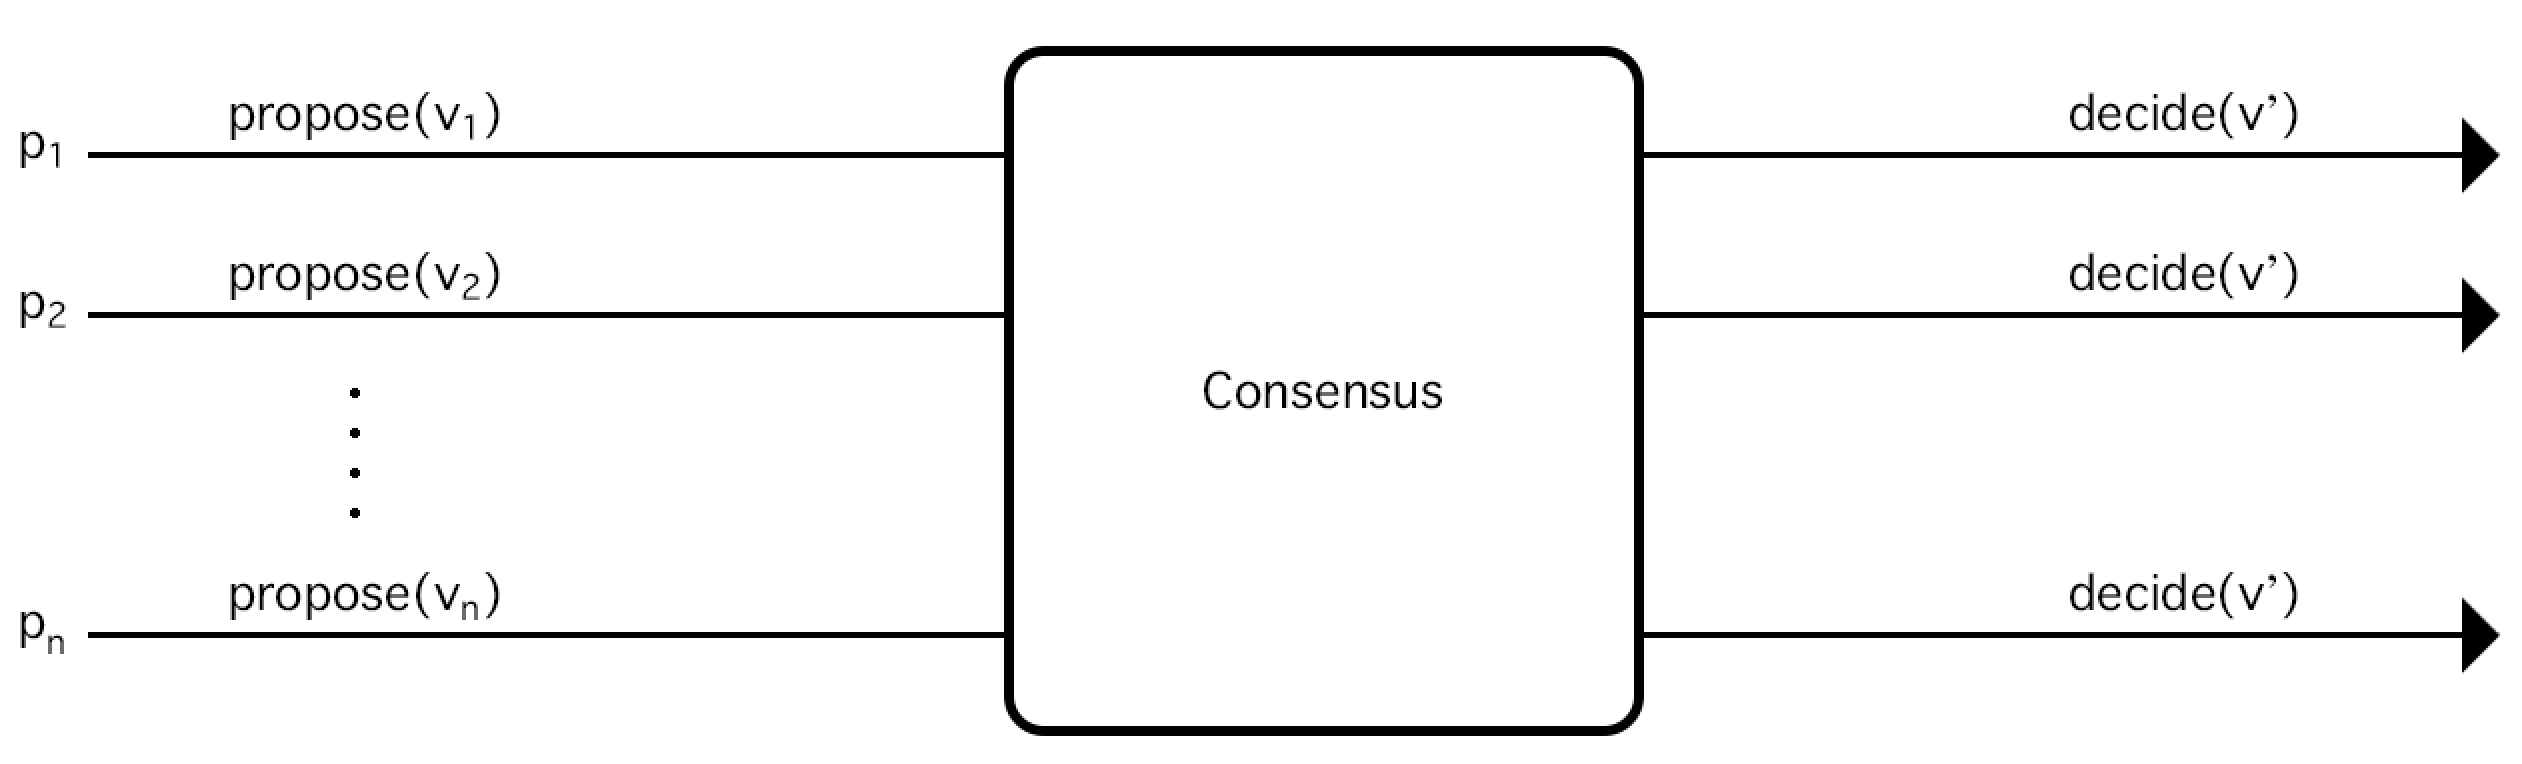
\includegraphics[width=\textwidth,height=\textheight,keepaspectratio]{img/consensus.png}

  \caption[The architecture of the system]{ The architecture of the system. The
    \textit{Viper IDE} and \textit{Viper Debugger} boxes denote, respectively,
    the main Viper extension and the new debugger extension. They both interact,
    independently, with Visual Studio Code. Viper Server is responsible for
    running the verification backends.}
  \label{fig:consensus}
\end{figure}

In this section we will go over some of the more relevant types of consensus, and respective implementations that are able to achieve consensus in the given system models.


\subsection{Synchronous model}\label{sec:Synchronous model}
In a synchronous system model, consensus is quite straightforward to achieve. Let us assume to have a set of $n$ processes, that will be the entities that want to reach a common agreement upon a proposed value. Let us also introduce the primitives used by the processes: each process is able to send and receive messages, through the primitives $send(m)$ and $receive(m)$ respectively, to communicate their intentions to the others. The failure model in a crash failure model, hence a correct process will never crash, while a faulty one eventually will; the number of faulty processes $f$.

Since we are in a synchronous model, we have a bound on the maximum time delay of a message, which means that a process is sure that if a message is sent, it will be received by the receiver before the maximum time delay. This is a quite strong and unrealistic model, but it makes the algorithm to solve consensus quite simple.

Let us have the algorithm proceed in rounds, where each round is as follows:
\begin{enumerate}
    \item Each process sends to all other processes a message containing information about its state.
    \item At the end of the round, after the maximum time bound, processes will have received a set of messages from a subset of all processes.
    \item The processes will then use the received messages together with its current state to reach a new state.
\end{enumerate}

The state can be simply a set values received until that moment, with the initial set containing only our own proposed value. Also, in a round a process can receive only a subset of messages from the other processes, since we can have up to $f$ faulty processes.

After $f+1$ rounds, we can be certain that each correct process will have enough information to deterministically decide on a single proposed value, and therefore reach consensus. This is because if we have a round where no process fails, then every process will receive all other values, and therefore we will be able to decide on a value. Also, since we have at most $f$ faulty processes, we can have at most $f$ rounds with a failing process. Therefore, we can be certain that $f+1$ rounds will be enough to reach agreement.

[should I put the lemmas properly?]

\subsection{Asynchronous model}\label{sec:Asynchronous model}
In this model, we have no bounds on process speed and maximum message delays; this means that a process if or when a message will be received by the other processes. This is a much weaker model compared to the previous one, and as a matter of fact it is proven that consensus cannot be solved in such a model [FLP proof].

\subsection{Alternative models}\label{sec:Alternative models}
The synchronous model allows us to solve consensus, but it's too strong of a model to be of any practical use. The asynchronous model cannot solve consensus. Therefore, we either have to find a system model that is weaker than synchronous and stronger than asynchronous, or we have to weaken the problem.

An alternative system model would be a partially-synchronous one, where the messages are asynchronous up to a GST (Global Stabilization Time), after which we can assume communication to become synchronous.

Another option is to still use an asynchronous system, but to also elect a process to be the leader and guide the whole decision procedure; an example of such an algorithm is Paxos, which is presented in the next section.

We could have failure detectors (which can be used with varying levels of completeness and accuracy), which could allow us to figure out when a process has failed, and therefore stoping us from waiting indefinitely for a message like in the basic asynchronous model.

An example of weaker problem definition would be to allow, for example, to have multiple values decided.

\section{Paxos}\label{sec:Paxos}
Paxos is an algorithm to achieve consensus that relies on an asynchronous system model, which makes it particularly interesting for real world application where we don't have completely reliable communication channels. To achieve this, the Paxos algorithm needs to elect one process as a leader that will act as a coordinator during the various phases of the protocol.

In Paxos, there are four types of process roles:
\begin{itemize}
  \item \textbf{Proposers} the processes that want to propose a value to be decided
  \item \textbf{Acceptors} the processes that take part in the voting part of the protocol; a quorum of acceptors is needed
  \item \textbf{Learners} the processes that, at the end of the algorithm, will be notified about the value decided by the algorithm
  \item \textbf{Leader} the process that acts as a coordinator
\end{itemize}

The election of the leader can be achieved in many different ways, as long as there is a point after which we have a unique correct process that is identified by the other processes as the leader.

The algorithm is divided into tree phases. During phase 1, a proposer that wants to propose a new value sends a new arbitrary value c-rnd higher than any previous c-rnd to the acceptors, so that all of them know that this is the most recent proposal attempt. Each acceptor, if the received c-rnd is truly the highest one it has received, replies to the proposer with its current state (rnd, v-rnd, v-val) so that the proposer know if there was already a previous proposed value, or if the proposer is allowed to propose its own.

In phase 2, once the proposer has received a reply from a quorum of acceptors, it checks if there was any acceptor that had previously voted for a value, and if this is the case, it picks the most recent one as the value to propose. If instead no acceptor had previously voted for a value, the proposer will be able to propose its own value. The proposer will then send to the acceptors the actual value to be proposed.
The acceptors, if the message of the proposer is still the most recent on-going proposal, will send back a message as an acknowledgement back to the proposer.

In phase 3, once the proposer receives again a quorum of replies from the acceptors, will be allowed to send to the learners the newly decided value.

The pseudo-code for the phases is as follows:
\begin{verbatim}
  c-rnd : highest-numbered round the process has started
c-val : value the process has picked for round c-rnd
% rnd : highest-numbered round the acceptor has participated, initially 0 v -rnd : highest-numbered round the acceptor has cast a vote, initially 0 v-val : value voted by the acceptor in round v-rnd, initially null
% To propose value v:
% increase c-rnd to an arbitrary unique value send (PHASE 1A, c-rnd) to acceptors
% upon receiving (PHASE 1A, c-rnd) from proposer if c-rnd > rnd then
% rnd ← c-rnd
% send (PHASE 1B, rnd, v-rnd, v-val) to proposer
% Phase 1B Phase 1A Acceptor Proposer
% upon receiving (PHASE 1B, rnd, v-rnd, v-val) from Qa such that c-rnd = rnd k ← largest v-rnd value received
% V ← set of (v-rnd,v-val) received with v-rnd = k
% if k = 0 then let c-val be v
% else c-val ← the only v-val in V
% send (PHASE 2A, c-rnd, c-val) to acceptors
% upon receiving (PHASE 2A, c-rnd, c-val) from proposer if c-rnd >= rnd then
% v-rnd ← c-rnd
% v-val ← c-val
% send (PHASE 2B, v-rnd, v-val) to proposer
% upon receiving (PHASE 2B, v-rnd, v-val) from Qa
% if for all received messages: v-rnd = c-rnd then
% send (DECISION, v-val) to learners
upon receiving (PHASE 1B, rnd, v-rnd, v-val) from Qa such that c-rnd = rnd k ← largest v-rnd value received
V ← set of (v-rnd,v-val) received with v-rnd = k
if k = 0 then let c-val be v
else c-val ← the only v-val in V
send (PHASE 2A, c-rnd, c-val) to acceptors
upon receiving (PHASE 2A, c-rnd, c-val) from proposer if c-rnd >= rnd then
v-rnd ← c-rnd
v-val ← c-val
send (PHASE 2B, v-rnd, v-val) to proposer
upon receiving (PHASE 2B, v-rnd, v-val) from Qa
if for all received messages: v-rnd = c-rnd then
send (DECISION, v-val) to learners
\end{verbatim}

\begin{itemize}
  \item \textbf{Termination} Eventually every correct process decides on one value
  \item \textbf{Uniform integrity} If a process decides on a value, then this value was proposed by some process
  \item \textbf{Uniform agreement} No two processes decide on a different value
  \end{itemize}

\begin{figure}[htb]
\centering
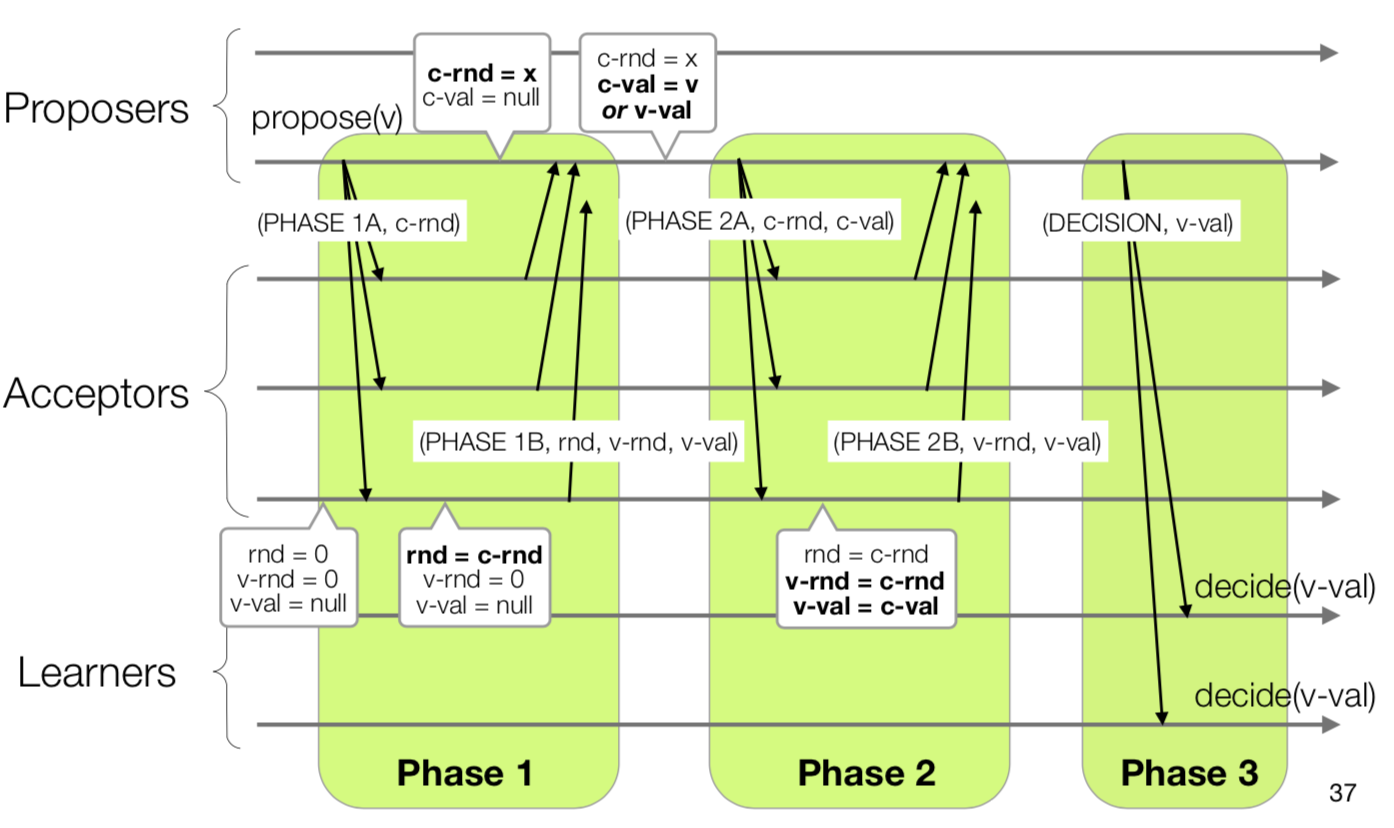
\includegraphics[width=\textwidth,height=\textheight,keepaspectratio]{img/paxos.png}

\caption[The architecture of the system]{ The architecture of the system. The
  \textit{Viper IDE} and \textit{Viper Debugger} boxes denote, respectively,
  the main Viper extension and the new debugger extension. They both interact,
  independently, with Visual Studio Code. Viper Server is responsible for
  running the verification backends.}
\label{fig:paxos}
\end{figure}

[should I add correctness, liveness, and so on?]

Remember that this algorithm allows only for the decision of one value; once value is decided, another instance of Paxos has to be initiated. Hence, for realistic use cases one would use system that allow to run multiple instances of paxos in a row, such as MultiPaxos.

The presented version of Paxos is the simplest one. Liveness in this case is not guaranteed; to ensure it, only the leader should be allowed to propose values, since otherwise it is possible that two proposers keep stealing their turn from each others without making any progress. Therefore the proposers should forward their values to the leader that will then try to propose them.

Various other improvements can be performed: for example, the leader could start phase 1 before a value is proposed, which means that once a value is ready to be proposed we can start directly from phase 2, virtually removing the delay of phase 1.
Also, at the end of Phase 2B the acceptors could send the decided value directly to the learners instead of having to first send it to the proposers; this allows to remove a whole message delay from the algorithm.

[should I write best message delays?]

\section{GeoPaxos}\label{sec:GeoPaxos}
Many current online services must serve clients distributed across geographic areas. In order to improve service avail- ability and performance, servers are typically replicated and deployed over geographically distributed sites (i.e., datacen- ters). By replicating the servers, the service can be configured to tolerate the crash of nodes within a single datacenter and the disruption of an entire datacenter. Geographic replication can improve performance by placing the data close to the clients, which reduces service latency.

Designing systems that coordinate geographically dis- tributed replicas is challenging. Some replicated systems resort to weak consistency to avoid the overhead of wide-area com- munication. Strong consistency provides more intuitive service behavior than weak consistency, at the cost of increased latency. Due to the importance of providing services that clients can intuitively understand, several approaches have been proposed to improve the performance of geo-distributed strongly consistent systems (e.g., [1], [2], [3], [4]). This paper presents GeoPaxos, a protocol that combines three insights to implement efficient state machine replication in geographically distributed environments.

First, GeoPaxos decouples ordering from execution [5]. Although Paxos introduces different roles for the ordering and execution of operations (acceptors and learners, respec- tively [6]), Paxos-based systems typically combine the two roles in a replica (e.g., [1], [2], [7]). Coupling order and execution in a geographically distributed setting, however, leads to a performance dilemma. On the one hand, replicas must be deployed near clients to reduce latency (e.g., clients can quickly read from a nearby replica). On the other hand, distributing replicas across geographic areas to serve remote clients slows down ordering, since replicas must coordinate to order operations. By decoupling order from execution, GeoPaxos can quickly order operations using servers in dif- ferent datacenters within the same region [1] and deploy geo- graphically distributed replicas without penalizing the ordering of operations.

Second, instead of totally ordering operations before execut- ing them, as traditionally done in state machine replication [8], GeoPaxos partially orders operations. It is well-known that state machine replication does not need a total order of operations [9] and a few systems have exploited this fact (e.g., [10], [2]). GeoPaxos differs from existing systems in the way it implements partial order. GeoPaxos uses multiple independent instances of Multi-Paxos [11] to order operations—hereafter, we call an instance of Multi-Paxos a Paxos group or simply a group. Operations are ordered by one or more groups, depending on the objects they access. Operations ordered by a single group are the most efficient ones since they involve servers in datacenters in the same region. Operations that involve multiple groups require coordination among servers in datacenters that may be far apart and thus perform worse than single-group operations. GeoPaxos’s approach to partial order can take advantage of public cloud computing infrastructures such as Amazon EC2 [12]: fault tolerance is provided by nodes in datacenters in different availability zones, within the same region; performance is provided by replicas in different regions. Although intra-region redundancy does not tolerate catastrophic failures in which all datacenters of a region are wiped out, most applications do not require this level of reliability [1].

Third, to maximize the number of single-group operations, GeoPaxos exploits geographic locality. Geographic locality presumes that objects have a preferred site, that is, a site where objects are most likely accessed. Geographic locality is common in many online services. For example, operations on a user’s data often originate in the region where the user is. Some distributed systems exploit locality by sharding the data and placing shards near the users of the data (e.g., [1], [4]). GeoPaxos does not shard the service state; instead, it distributes the responsibility for ordering operations to Paxos groups deployed in different regions. Operations are ordered by the groups in the preferred sites of the objects accessed by the operation.

The rest of the paper is structured as follows. Section II details the system model and recalls fundamental notions. Section III overviews the main paper contributions. Section IV
details GeoPaxos. Section V describes our prototype. Sec- tion VI presents our performance evaluation. Section VII reviews related work and Section VIII concludes the paper.

[add better explanations of the things]
[add images]
\chapter{GeoPaxos with B+tree}\label{sec:geopaxos-with-B+tree}
Now that we have discussed the needed background, we can move onto the next step: using a B+tree \citep{b+tree} on top of GeoPaxos to store the data objects. A B+tree has many interesting characteristics that make it particularly suitable for some types of applications, but it also brings some new challenges to the table. The data structure has to be indentical in every replica: this means that all the operations done on the tree have to be deterministic and executed in the right order. While this is not particularly complicated on other data structures, such as a HashMap, this becomes more complicated with a tree, where we have many branches and nodes that may split and cause further modifications up to the root.

Furthermore, the usage of GeoPaxos with a tree brings the need for a new type of operation. In GeoPaxos the objects are assigned to one or more groups, or partitions, depending on the type, number and origin of accesses. Of these groups, one will also be chosen in each replica to be the preferred partition for the operation, usually based on geographic location. There has to be a moment when these groups are decided and calculated for each object in the B+tree. For this, we have a command called repartition. The command takes the workload of an object, which is the number of reads and writes from each group on this object, and a graph that represents the geographic location of the various replicas. It then calculates the optimal placement of the object in the groups, that with the given workload would give us the minimum average latency. As a reminder, we do \textbf{\emph{not}} partition the B+tree. The tree is fully replicated in all the distributed replicas. What we want to partition is the responsibility of ordering the operations for the objects in the B+tree.

This operation can be a big performance bottleneck, since it has to be executed for every object in the tree. Furthermore, each group can either be responsible or not responsible for the operations on an object. This means that for every object, if we have $m$ groups, we have $2^m$ possible combinations of assignments of responsibility, which means that the repartition optimization grows exponentially with the number of groups. We therefore want to find a fast way to perform this operation so that we still get the right assignment of objects in a short amount of time.

In the following sections of this chapter we will first explain what a B+tree is, how it works and what are its advantages and disadvantages. We will then describe the specific B+tree used in our application. Then we will go over the various approaches that were attempted to improve the performance of the repartition optimization, followed with tests on the performance of the repartition operation only and finally with GeoPaxos as well.

\section{B+tree}\label{sec:B+tree}
The B+tree is the data structure that was chosen to store the data in the geo-replicated servers. Since the B+tree is a special case of a B-tree \citep{b-tree}, let us quickly mention what a B-tree \citep{b-tree} is.

A B-tree is a self-balancing data structure; it is a more general version of a binary search tree, since it allows nodes to have an arbitrary number of children, instead of two like in a binary search tree. Its advantage is that one node can have an increased number of children (this number being called the \emph{branching factor}), making it more efficient to retrieve large amounts of data at once. Also, its time complexities for search, insertion and deletion are $O(log\ n)$, where $n$ is the number of objects in the tree.

A B+tree is similar to a B-tree, but all its data items are stored at the leaves of the tree. It has three types of nodes: the root node, the inner nodes and the leaves. The leaves are the nodes at the lowest level of the tree, level 0, and that can only point to data items; inner nodes can be found from levels higher than 0, and they point to other inner nodes or to leaf nodes. The root is a special case, as it is initially a leaf node when the tree is empty, but when the tree starts to fill up it will act as an inner node. Also, the branching factor of a B+tree can be quite high, particularly compared to a B-tree. In our implementation, for example, we use a branching factor of $b=100$.

The main advantage of the B+tree, similarly to a B-tree, is when it comes to accessing big amounts of data at once. Say, for example, that we want to perform some operation on a range of elements. Since the data items are all at the leaves and grouped together, we can retrieve at once hundreds of data items with few operations.

Give a branching factor of $b$, leaf nodes and inner nodes can have a number of children between $\lceil b/2 \rceil$ and $b$. This means that in our implementation, with $b=100$, leaf nodes and inner nodes will always have between 50 and 100 children. The exception is the root, which initially will have only one child, and it will act as a leaf. Once it reaches $b-1$ data items, two inner nodes are created, they become children of the root and they get half of the data items each; at this point, the root will start acting like an inner node, with a minimum of 2 children up to $b$.

The splitting of nodes is similar to other self-balancing trees: when a node reaches the maximum number of children allowed by the maximum branching factor, a new node is created, and half of the children of the full node are given to the new node. Since then the new node has to be appended to the parent's children, a split may propagate up to the root of the tree.

Figure \ref{fig:B+tree} shows a B+tree with a branching factor of $b=4$. We have a root node that acts as an inner node, which means that its children are nodes themselves. The children nodes are leaf nodes, with their children being the actual objects that are being stored.

\begin{figure}[!htb]
    \centering
    \includegraphics[width=\textwidth,height=\textheight,keepaspectratio]{img/B+tree.png}
    \caption{ An example of B+tree }
    \label{fig:B+tree}
\end{figure}

% [add characteristics from wiki?]

\subsection{B+tree implementation}\label{sec:B+tree-implementation}
For our application, the basic B+tree needs to have some extra characteristics added to it. We will now explain the details of how our specific B+tree implementation works.


\subsubsection{Regions and groups}
Let us start by quickly explaining what regions and groups are. We can imagine the regions as the clusters, or areas, where the latencies between entities are low, and such that the latencies between regions are noticeable. In the real world, these regions often correspond to geographical regions.

A simple idea of regions can be found in Amazon EC2 \citep{amazonEC2}, that offers its service in a multitude of different regions: \textbf{US East} (N. Virginia, Ohio), \textbf{US West} (N. California, Oregon), \textbf{Canada} (Central), \textbf{EU} (Frankfurt, Ireland, London, Paris, Stockholm), \textbf{Asia Pacific} (Hong Kong, Tokyo, Seoul, Osaka-Local, Singapore, Sydney, Mumbai, \textbf{South America} (S$\tilde{a}$o Paulo).

The decision of how big a region is depends both on the geographic distance between regions and on the number of clients in that region.\\\\
GeoPaxos uses a multitude of Multi-Paxos instances, called Paxos groups or just groups, to perform the ordering of operations. The system does not, inherently, have a notion of regions, but only groups. While groups and regions are two different things, though, we will often just deploy a group for each region, so that we have one group responsible for the ordering of each region. Because of this, in some situations we will sometimes use the two terms in an almost interchangeable way, but it is important to remember that they are two distinct concepts.

\subsubsection{RW counters}
Each node (root, inner and leaf nodes) will count the read and write operations based on the operations performed on its child objects. In the following sections, we will refer to those counters as \textbf{\emph{RW counters}}. In particular, each node will have two counters, one for read and one for write operations, for each group in the system. Therefore, if we have three groups, each node will have six counters. The RW counters are updated from the root up to the node that handles the item accessed. In Figure \ref{fig:B+tree_path} we can see in red the nodes that will have their RW counters updated upon we perform an operation on object X. 

\begin{table}[!htb]
  \centering
  \begin{tabular}{l l l l}
    \hline
    & \textbf{Group 1} & \textbf{Group 2} & \textbf{Group 3} \\
    \hline
    \textbf{Reads} & 150 & 37 & 540 \\
    \textbf{Writes} & 32 & 10 & 93 \\
    \hline
  \end{tabular}
  \caption{The six RW counters of a node that make up its workload}\label{tab:workload-example}
\end{table}

\begin{figure}[!htb]
  \centering
  \includegraphics[width=\textwidth,height=\textheight,keepaspectratio]{img/B+tree_path.png}
  \caption{ The nodes whose RW counters are updated when there is an operation on object X }
  \label{fig:B+tree_path}
\end{figure}

These RW counters will be used as \textbf{\emph{workload}} when the repartition is issued. Once the repartition is performed, each RW counter will be updated with the following formula:
$$ current\_RW counter = \alpha \cdot old\_RW counter + (1-\alpha) \cdot new\_RW counter $$
Where the old RW counters are the ones gathered until the past repartition, and the new RW counters are the ones between the past repartition and the current one (In Figure \ref{fig:RW counters} we can see an example of how the RW counters are updated for each node after every repartition, with $\alpha = 0.5$).
$\alpha$ is the aging factor, which determines how much importance we give to the old and new RW counters. A small $\alpha$ gives more weight to recent ones, but it also makes the system more susceptible to unexpected variations in the workloads.

\begin{figure}[!htb]
  \centering
  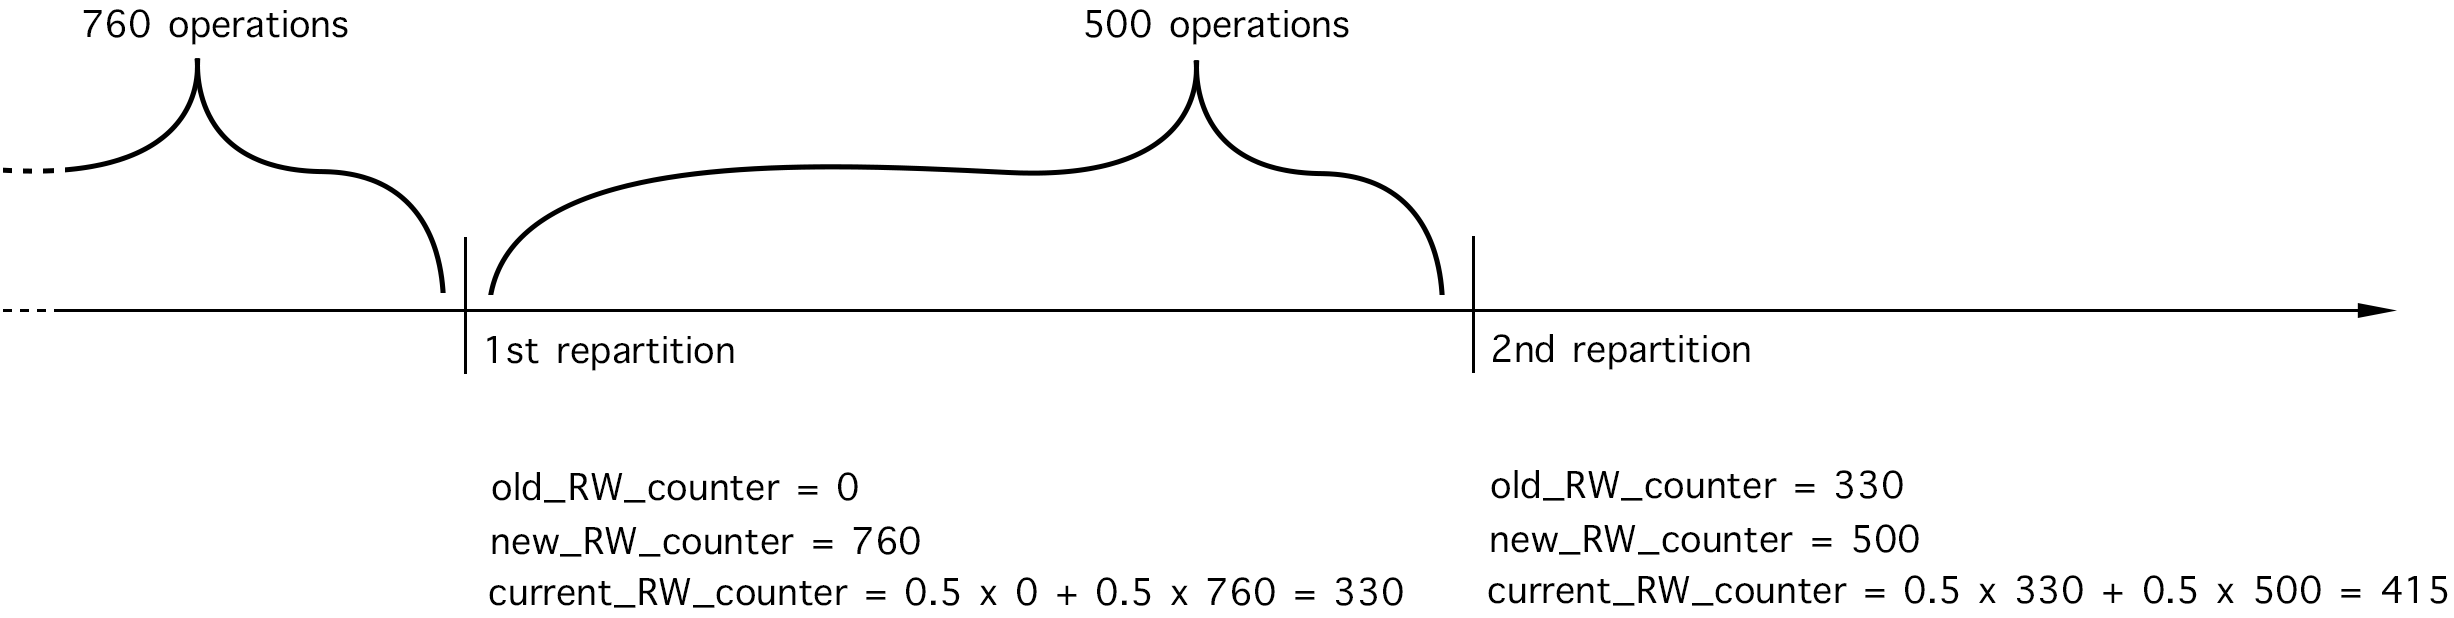
\includegraphics[width=\textwidth,height=\textheight,keepaspectratio]{img/RW_counters.png}
  \caption{ The update done for each RW counter upon repartition }
  \label{fig:RW counters}
\end{figure}

Furthermore, whenever a node is full and it has to split, its RW counters are halved evenly between the two nodes. This is because we do not know which RW counters correspond to which data item in particular, but we can assume that there is a decent chance that objects that are close to each other will have similar RW counters, which means that we expect them to have good locality.

\subsubsection{Partitions}
The second thing that we need to store in the nodes of our B+tree are the partitions. In particular, we need to store both the \textbf{\emph{partitions}} that take care of each node and the \textbf{\emph{preferred partition}} in case there are multiple partitions to choose from. Initially, each new node will be assigned to all partitions of the system. This is to make sure that all clients will initially have the same availability of the data items. Once we issue a repartition, the algorithm will calculate the optimized partitions for each node based on the workload. These optimal repartition will be used to know which replicas to involve in the subsequent operations on each object, until the next repartition.

If a node splits, the new node will inherit the partitions from the full node. This is again a heuristic, based on the high likelihood that close objects will have similar accesses.

\subsection{System implementation}\label{sec:system-implementation}
The implementation of the B+tree data structure, the repartition algorithms and the further code necessary to use this structure on top of GeoPaxos was written in C++. Since this is built on top of the GeoPaxos library, there is also the requirement for the libraries needed by GeoPaxos itself, in particular libevent \citep{libevent} for the networking part, libpaxos for consensus \citep{libpaxos} and libmcast \citep{libmcast} for atomic multicast.

\chapter{Optimization approaches}\label{sec:optimization-approaches}
In this section we will first explain in detail how we calculate the optimized group assignment of data objects to the partitions based on the workload. We will then go over the various approaches that were attempted to improve the repartition process. 

\section{Optimal partitions algorithm}\label{sec:optimal-partitions-algorithm} 
The simplest algorithm to come up with is the one that compares all the possible combinations of partitions and picks the best one. While this algorithm will give the optimal assignments for minimum average latency for a certain workload, it is also the one that takes the largest amount of time. We will use the performance of this algorithm as a benchmark to compare against our later algorithms.

Also be aware that in this context, with ``optimal'' we refer to the best solution based on how we defined the problem. There are many values to optimize for (e.g., lowest maximum latency, lowest average latency, maximum throughput...) and even for the same variable to optimize, there are multiple ways to do it. Therefore keep in mind that with optimal we just mean the best partitioning given our optimization function.

The pseudocode of this algorithm can be found in Algorithm \ref{alg:all-combinations}. This algorithm goes top to bottom and it calculates the partitions for each node. The workload of a node will have a structure similar to the one shown in Table \ref{tab:workload-example}. In the table we can see a workload example for a node in a case with three groups; the node counts the number of read and write operations received from each group, to be used for the repartition algorithm.

\begin{table}[!htb]
  \centering
  \begin{tabular}{l l l l}
    \hline
    & \textbf{Group 1} & \textbf{Group 2} & \textbf{Group 3} \\
    \hline
    \textbf{Reads} & 150 & 37 & 540 \\
    \textbf{Writes} & 32 & 10 & 93 \\
    \hline
  \end{tabular}
  \caption{Example of a possible workload of a node}\label{tab:workload-example}
\end{table}

We then build a graph that represents the geographic placements of the various replicas, where the cost of the edges is the estimated average round trip time required to send a message. In Figure \ref{fig:graph} we have a graph representing a geographically distributed environment. Each of the three groups are placed far away, with round trip times defined between each pair of groups. Each group will have multiple replicas in its area, with negligible latency.

\begin{figure}[!htb]
  \centering
  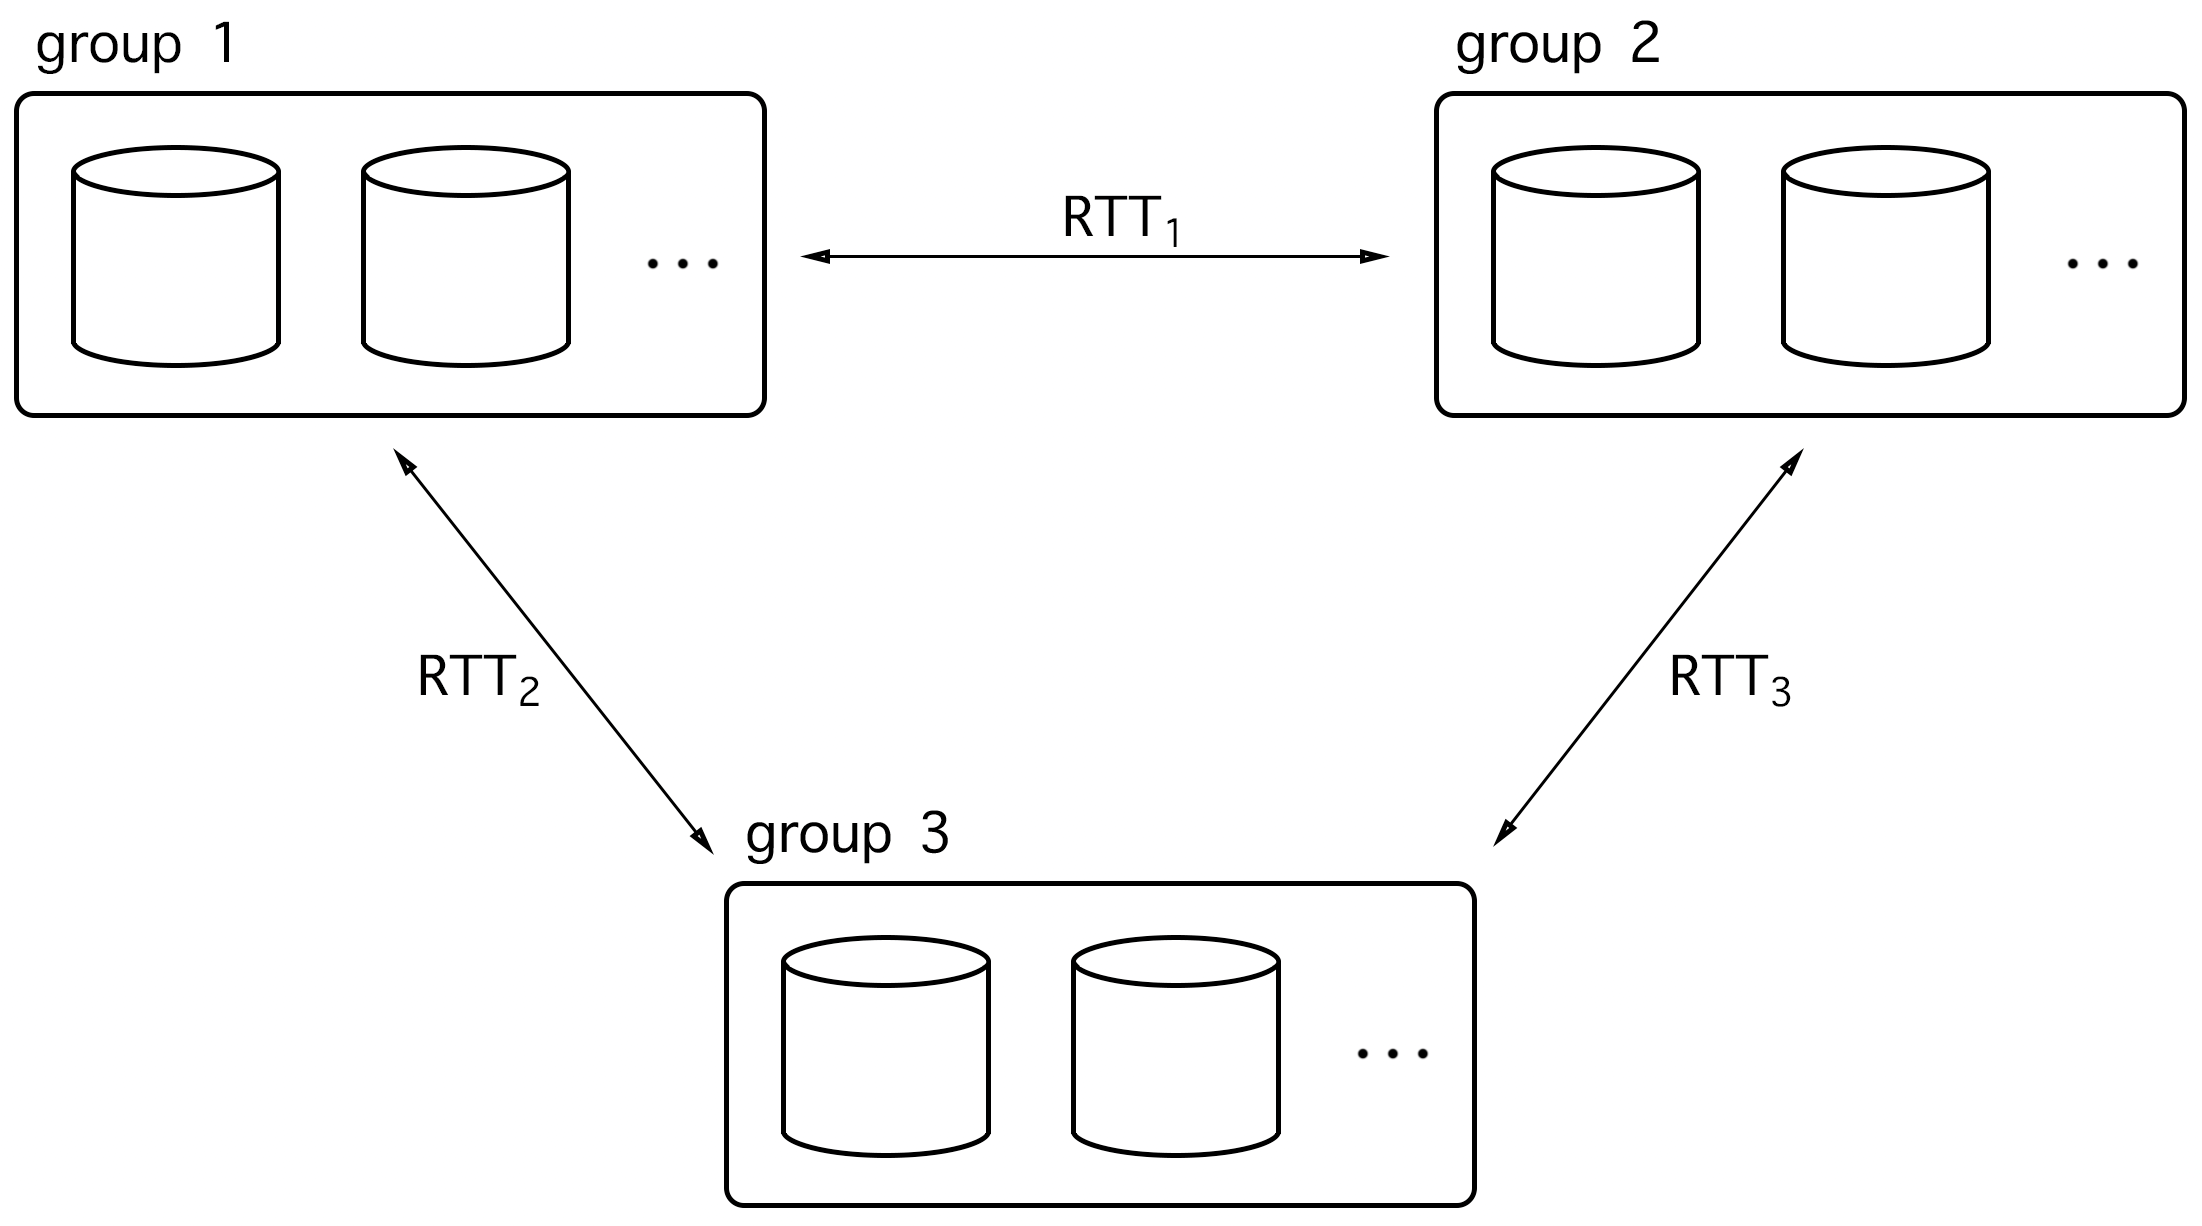
\includegraphics[width=\textwidth,height=\textheight,keepaspectratio]{img/graph.png}
  \caption{An example graph}
  \label{fig:graph}
\end{figure}

Once we have the graph, we proceed by looping over all possible combinations of groups, where a group can be either taken or not taken. Logically, at least one group has to be taken, since we need the object to be assigned to at least one group. In the case of 3 groups, we would have to consider $2^3 -1 = 7$ combinations: $001, 010, 100, 011, 101, 110, 111$, where 1 and 0 mean that the object will be or will not be assigned to that specific replica.

Given the number of reads and writes for each group, and the current groups to which we are replicating this object, we multiply the number of reads by the latency with the closest replica that would have this object. For writes, we have to add the latency of all the replicas that have this object, since the operation is going to modify the data item in all involved regions.

Also note that the result depends on the latency that we are currently considering: for example, if we do the calculations from the point of view of a replica that will not have this object, each read will have to go to a different replica; therefore we have to consider the costs from the point of view of all the replicas.

Once we have gone over all the combinations, we pick the one with the lowest cost, and we move onto the next object.

\begin{algorithm}
  \caption{All-combinations}\label{alg:all-combinations}
  \begin{algorithmic}[1]
  \Function{repartition}{}:
  \State $repartition\_tree(root)$
  \EndFunction
  \Function{repartition\_tree}{$node$}:
    \If {$node.has\_changed$}:
      % \State $vw = vector(node.statistics)$
      \State $topology = new\ topology(node.workloads)$
      \State $min\_graph =  topology.calculate\_min\_cost\_graph()$
      \For {$vertex \in min\_graph$}:
        \If {$vertex.has\_obj$}:
        \State $node.partitions += vertex$
          \If {$vertex == my\_partition\ \wedge vertex.has\_obj$}:
            \State $node.preferred\_partition = vertex$
          \EndIf
        \EndIf
      \EndFor
    \EndIf
    \If{$!node\ is\ leafnode$}:
      \For {$child\ \in\ node.child\_nodes$}:
        \State $repartiton\_tree(child)$
        \EndFor
    \EndIf
    \EndFunction
    \Function{calculate\_min\_cost\_graph}{}:
    \State $min\_cost = \infty$
      \ForAll {$graph\ combination$}:
        \State $cost = calculate\_cost(graph, vertices)$
        \If {$cost < min\_cost$}:
          \State $min\_cost = cost$
          \State $min\_graph = graph$
        \EndIf
      \EndFor
    \State \textbf{return} $min\_graph$
    \EndFunction
    \Function{calculate\_cost}{$graph,\ vertex$}:
      \State $in\_reads, out\_reads, in\_writes, out\_writes = 0$
      \State $replicas = [vertex \in graph.vertices \mid vertex.has\_obj$]
      \For {$vertex \in graph.vertices$}:
      \State $min\_weight = dist(nearest\ vertex \in graph\ |\  vertex.has\_obj)$
      \State $max\_weight = dist(furthest\ vertex \in graph\ |\ vertex.has\_obj)$
        \If {$vertex.has\_obj$}:
          \State $in\_reads+= 1$
          \If {$replicas.size > 1$}:
          \State $in\_writes+= vertex.writes$
          \Else:
          \State  $in\_writes+= 1 $
          \EndIf
        \Else:
          \State $out\_reads += vertex.reads \cdot min\_weight$
          \State $out\_writes += vertex.writes \cdot min\_weight$
        \EndIf
      \EndFor
      \State $cost = in\_reads+ out\_reads + (in\_writes+ out\_writes) \cdot max\_weight$
      \State \textbf{return} $cost$
  \EndFunction
  \end{algorithmic}
  \end{algorithm}

\section{Fixed-size buckets}\label{sec:fixed-size buckets}
One of the ideas to improve the performance of the repartition is to try to reduce the number of nodes that we have to do the calculations for.

Since the tree is divided in levels, the idea is to group nodes of different levels in what we call \textbf{\emph{buckets}} and do an aggregated calculation of the optimal partition assignment for the whole bucket. An example of a bucket can be seen in Figure ~\ref{fig:fixed-size-buckets}. The pseudocode can be found in Algorithm \ref{alg:fixed-size}.

As a reminder, whenever a operation is performend on an object, the RW counters of the tree are updated along the whole path from the root to the node that handles this object. This means that in general, the parent node will have the aggregated RW counters for all its children nodes (this may not always be the exact case when the parent node splits, but this is quite rare, and even when it happens the RW counters of the split nodes are good approximations of the real RW counters).

There are also multiple ways to group nodes in the case where we have an odd number of levels. Since we are using buckets of two levels, we could either allow the root node to be a bucket of 1 level, or let the leaves be buckets of 1 level. Or, we could have the root be the only bucket to be allowed to have 3 levels. The first one would not reduce the number of saved calculations by much, since most nodes are on level 0; the other two options make virtually no difference, as they only affect the level with the least amount of nodes. We decided to go with the second option, allowing the root node to be in a bucket of its own in case of an odd number of levels.

It is also important to remember that this improvement affects only the number of objects, not the groups; therefore, in the case where we have $n$ objects and $m$ groups, this would improve on the linear number of objects $n$ but it would not affect the number of combinations, which grows as $2^m$.

In general, given a branching factor $b$ of and $n$ objects, the number of calculations we would be doing would be around $\approx\cfrac{n}{b}$ as the tree grows, since we are approximating all the calculations at level 0, which is by far the level with the most nodes.

This approach will generally work best in cases where we have a great amount of locality, which means that the heuristic of grouping nodes together expecting them to have similar behavior would be mostly correct. Even in that case, though, we expect to still see repartitioning results that are not optimal.

Figure \ref{fig:fixed-size-buckets} shows a visualization of how the levels are grouped. The nodes in the same triangles are going to have the same partitioning, based on the aggregated RW counters (which are going to be the RW counters of the highest-level node). The root at level 2 is in its own bucket, since we have an odd number of levels. Also note that only a few nodes are shown too keep the visualization simple.

\begin{figure}[!htb]
  \centering
  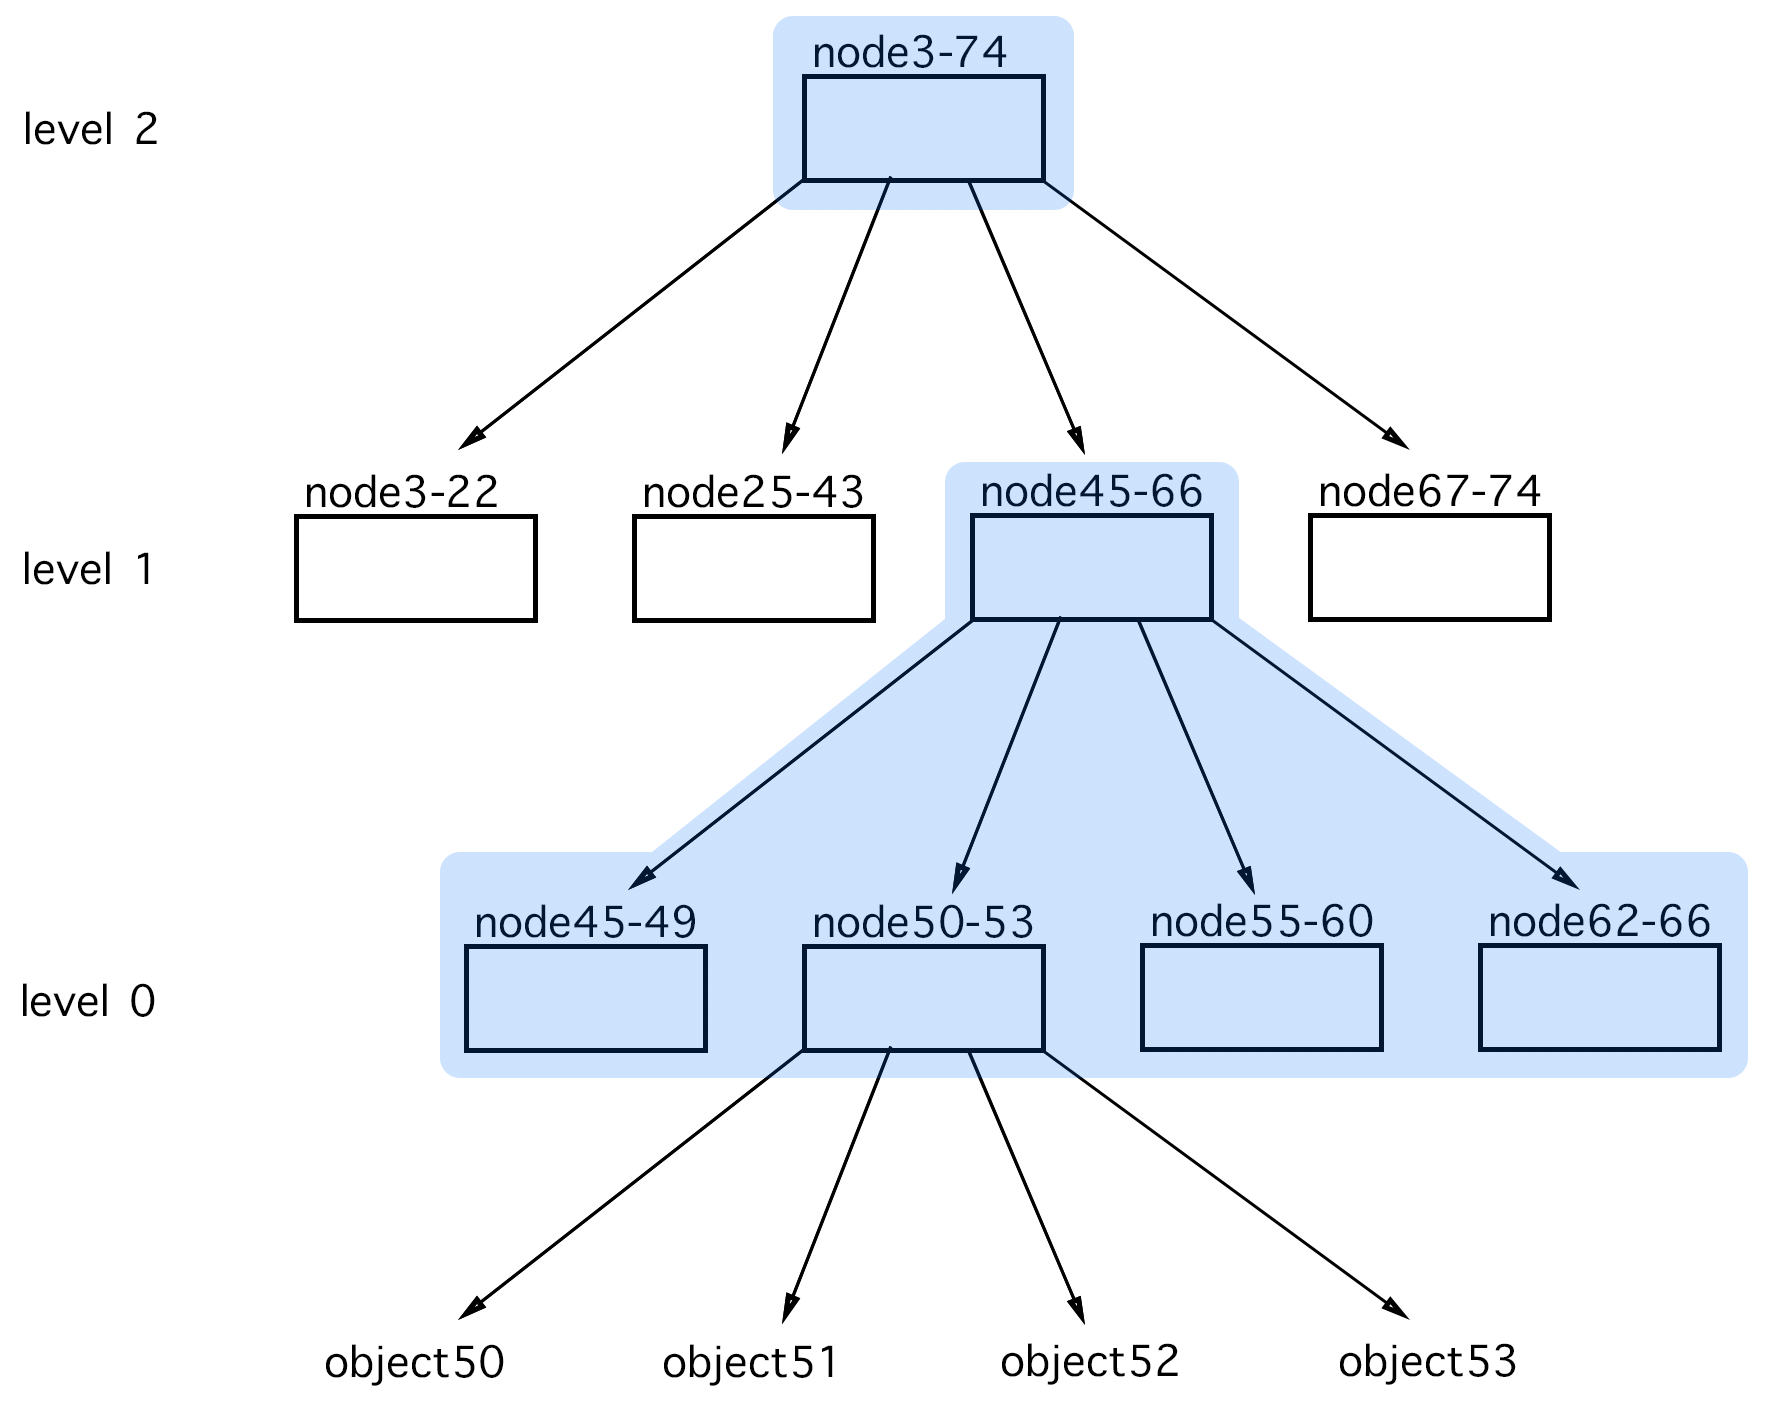
\includegraphics[width=\textwidth,height=\textheight,keepaspectratio]{img/grouped-levels.png}
  \caption{ The grouping of levels with fixed-size buckets}
  \label{fig:fixed-size-buckets}
\end{figure}

\begin{algorithm}
  \caption{Fixed-size Buckets}\label{alg:fixed-size}
  \begin{algorithmic}[1]
    \Function{repartition}{}:
  \State $repartition\_tree(root, true)$
  \EndFunction
  \Function{repartition\_tree}{$node, is\_root$}:
  \State $is\_bucket\_root = node.level\ is\ odd \vee is\_root$
    \If {$node.has\_changed \vee is\_bucket\_root$}:
      % \State $vw = vector(node.statistics)$
      \State $topology = new\ topology(node.workloads)$
      \State $min\_graph =  topology.calculate\_min\_cost\_graph()$
      \For {$vertex \in min\_graph$}:
        \If {$vertex.has\_obj$}:
        \State $node.partitions += vertex$
          \If {$vertex == my\_partition\ \wedge vertex.has\_obj$}:
            \State $node.preferred\_partition = vertex$
          \EndIf
        \EndIf
      \EndFor
    \EndIf
    \If{$!node\ is\ leafnode$}:
      \For {$child\ \in\ node.child\_nodes$}:
      \If {$is\_bucket\_root = node.level\ is\ odd$}:
        \State $child.partitions = node.partitions$
        \State $child.preferred\_partition = node.preferred\_partition$
      \EndIf
        \State $repartiton\_tree(child, false)$
        \EndFor
    \EndIf
    \EndFunction
    \Function{calculate\_min\_cost\_graph}{}:
    \State $min\_cost = \infty$
      \ForAll {$graph\ combination$}:
        \State $cost = calculate\_cost(graph, vertices)$
        \If {$cost < min\_cost$}:
          \State $min\_cost = cost$
          \State $min\_graph = graph$
        \EndIf
      \EndFor
    \State \textbf{return} $min\_graph$
    \EndFunction
    \Function{calculate\_cost}{$graph,\ vertex$}:
      \State $in\_reads, out\_reads, in\_writes, out\_writes = 0$
      \State $replicas = [vertex \in graph.vertices \mid vertex.has\_obj$]
      \For {$vertex \in graph.vertices$}:
      \State $min\_weight = dist(nearest\ vertex \in graph\ |\  vertex.has\_obj)$
      \State $max\_weight = dist(furthest\ vertex \in graph\ |\ vertex.has\_obj)$
        \If {$vertex.has\_obj$}:
          \State $in\_reads+= 1$
          \If {$replicas.size > 1$}:
          \State $in\_writes+= vertex.writes$
          \Else:
          \State  $in\_writes+= 1 $
          \EndIf
        \Else:
          \State $out\_reads += vertex.reads \cdot min\_weight$
          \State $out\_writes += vertex.writes \cdot min\_weight$
        \EndIf
      \EndFor
      \State $cost = in\_reads+ out\_reads + (in\_writes+ out\_writes) \cdot max\_weight$
      \State \textbf{return} $cost$
  \EndFunction
  \end{algorithmic}
  \end{algorithm}

\section{Variable-size buckets}\label{sec:Variable-size buckets}
The idea of the fixed-size buckets is interesting, as it greatly reduces the number of nodes we have to account for, but it also generalizes the situation, grouping the nodes regardless of their workload. Reducing the branching factor would not be a solution, as it would just increase the number of nodes once again, and because the high branching factor is one of the main reasons to use a B+tree. 

An alternative approach is to to have a variable, or dynamic, size of buckets. The idea is to group in two or more levels the nodes that have a low amount of RW counters, and instead do the optimal calculations for the nodes with many operations associated to them. The idea is that approximating the nodes with few operations would not hinder the performance by much, as the object associated to those nodes will not be accessed often by the clients, while instead the objects that are accessed often will have their optimal partitions. 
The pseudocode for this method is in Algorithm \ref{alg:variable-size}.


One challenge of the Variable-size buckets approach is to figure out when it is worth doing the full calculations and when it is better to group in buckets. In the case where the operations are evenly distributed among all children of a node, we would expect that the RW counters of a child node will be around $\cfrac{1}{b}$ of the parent node. Then, we could say that if, for example, a child node has less than $\cfrac{1}{b^2}$, then we should place it in a bucket; but finding the right number depends on many variables and on the system at hand, therefore finding a good value would have to be fine-tuned depending on the application.

We can see an example in Figure \ref{fig:Variable-size-buckets}. Node 45-66 has few operations, therefore it will group all its children into one bucket. Node 67-74 instead has more operations, therefore performing a better partitioning might give us better improvements; therefore, this node will not group its children, and we will calculate the optimal partition for those nodes. 

\begin{figure}[!htb]
  \centering
  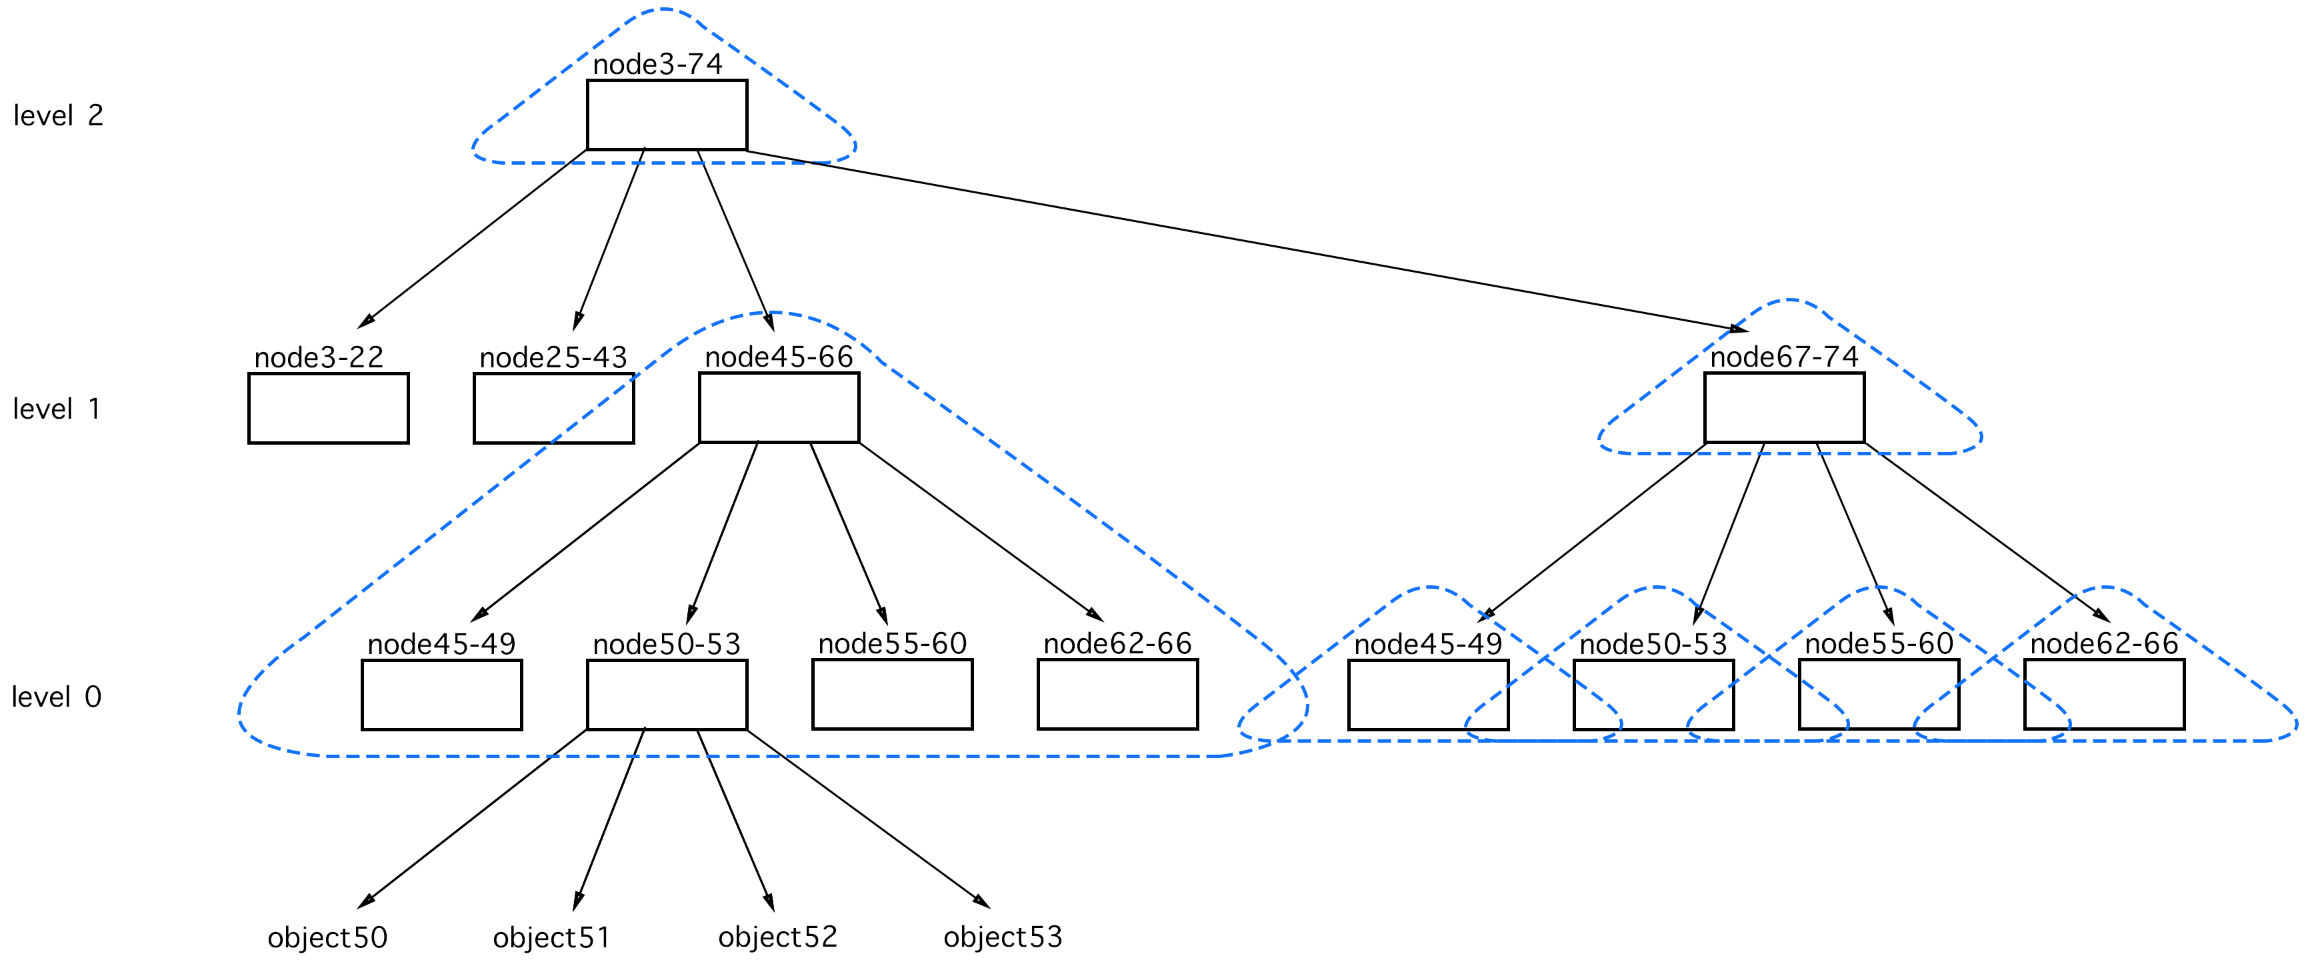
\includegraphics[width=\textwidth,height=\textheight,keepaspectratio]{img/dynamic-buckets.png}
  \caption{ The grouping of levels with variable-sized buckets}
  \label{fig:Variable-size-buckets}
\end{figure}

\begin{algorithm}
  \caption{Variable-size Buckets}\label{alg:variable-size}
  \begin{algorithmic}[1]
    \Function{repartition}{}:
  \State $repartition\_tree(parent\_node, workload\_ratio)$
  \EndFunction
  \Function{repartition\_tree}{$node, is\_root$}:
    \State $my\_workload = 0$
    \If {$node.has\_changed$}::
      \State $my\_workload = sum(node.workloads)$
      \If {$my\_workload < workload\_ratio * treshold$}:
      \State $child.partitions = parent.partitions$
      \State $child.preferred\_partition = parent.preferred\_partition$
      \Else
      \State $topology = new\ topology(node.workloads)$
      \State $min\_graph =  topology.calculate\_min\_cost\_graph()$
      \For {$vertex \in min\_graph$}:
        \If {$vertex.has\_obj$}:
        \State $node.partitions += vertex$
          \If {$vertex == my\_partition\ \wedge vertex.has\_obj$}:
            \State $node.preferred\_partition = vertex$
          \EndIf
        \EndIf
      \EndFor
    \EndIf
    \EndIf
    \If{$!node\ is\ leafnode$}:
      \For {$child\ \in\ node.child\_nodes$}:
        \State $repartiton\_tree(child, false)$
        \EndFor
    \EndIf
    \EndFunction
    \Function{calculate\_min\_cost\_graph}{}:
    \State $min\_cost = \infty$
      \ForAll {$graph\ combination$}:
        \State $cost = calculate\_cost(graph, vertices)$
        \If {$cost < min\_cost$}:
          \State $min\_cost = cost$
          \State $min\_graph = graph$
        \EndIf
      \EndFor
    \State \textbf{return} $min\_graph$
    \EndFunction
    \Function{calculate\_cost}{$graph,\ vertex$}:
      \State $in\_reads, out\_reads, in\_writes, out\_writes = 0$
      \State $replicas = [vertex \in graph.vertices \mid vertex.has\_obj$]
      \For {$vertex \in graph.vertices$}:
      \State $min\_weight = dist(nearest\ vertex \in graph\ |\  vertex.has\_obj)$
      \State $max\_weight = dist(furthest\ vertex \in graph\ |\ vertex.has\_obj)$
        \If {$vertex.has\_obj$}:
          \State $in\_reads+= 1$
          \If {$replicas.size > 1$}:
          \State $in\_writes+= vertex.writes$
          \Else:
          \State  $in\_writes+= 1 $
          \EndIf
		  \algstore{variable}
		\end{algorithmic}
	\end{algorithm}
	\begin{algorithm}
		\begin{algorithmic}[1]
			\algrestore{variable}
        \Else:
          \State $out\_reads += vertex.reads \cdot min\_weight$
          \State $out\_writes += vertex.writes \cdot min\_weight$
        \EndIf
      \EndFor
      \State $cost = in\_reads+ out\_reads + (in\_writes+ out\_writes) \cdot max\_weight$
      \State \textbf{return} $cost$
  \EndFunction
  \end{algorithmic}
  \end{algorithm}

\section{Hot groups}\label{sec:hot-groups}
Another option is to try to reduce the number of combinations that we have to consider for each node. Since the complexity grows exponentially with the number of groups, if we are able to discard some combinations before we calculated their actual cost, then we should have a greater improvement compared to the optimizations that reduce the number of nodes.

One idea to do this is as follows: given a workload, there is a chance that one or more groups will have fewer operations on the current node compared to other groups. Then, there is a big chance that the final partition assignment would not assign the objects to the group with fewer operations, since the gain of replicating the object to said partition would be less than the added cost of it.

The cost of replicating to a group with few operations also depends on the ratio between read and write operations: with many reads we would want to assign the object to all groups, while with many writes we would want to reduce the number of group assignments for each object, as with every write we would have to coordinate between all groups involved. In general, though, such a system is better suited for applications with more reads than writes, therefore our assumption of discarding groups with few operations still holds.

The way to implement this is fairly simple: with the workload at hand, we find the group or groups with the highest number of operations (the \textbf{\emph{hot groups}}). Then, when we are going through all the possible combinations of groups, we discard those that would assign the object to groups with much lower operations than the hot groups.  See Algorithm \ref{alg:fixed-size} for the pseudocode.

As before, finding the ideal threshold is not an easy task; a higher threshold would discard more combinations, making the computations faster but possibly lose a lot of accuracy, while a lower threshold might only skip very few combinations giving us very small performance improvements. 

Table \ref{tab:hot-groups-example} is a possible workload of a node in a case with 3 groups. In this case, group 3 would be the hot group, since it is the node with more total operations. Depending on the threshold, we could discard only group 2 or both group 1 and 2 from the list of possible assignment combinations; this would reduce the number of combinations for this node from 7 to 3 or 1, respectively.


\begin{table}[!htb]
  \centering
  \begin{tabular}{l l l l}
    \hline
    & \textbf{Group 1} & \textbf{Group 2} & \textbf{Group 3} \\
    \hline
    \textbf{Reads} & 150 & 37 & 540 \\
    \textbf{Writes} & 32 & 10 & 93 \\
    \hline
  \end{tabular}

  \caption{ An example workload }\label{tab:hot-groups-example}
\end{table}

\begin{algorithm}
  \caption{Hot groups}\label{alg:hot-groups}
  \begin{algorithmic}[1]
  \Function{repartition}{}:
  \State $repartition\_tree(root)$
  \EndFunction
  \Function{repartition\_tree}{$node$}:
    \If {$node.has\_changed$}:
      % \State $vw = vector(node.statistics)$
      \State $topology = new\ topology(node.workloads)$
      \State $min\_graph =  topology.calculate\_min\_cost\_graph()$
      \For {$vertex \in min\_graph$}:
        \If {$vertex.has\_obj$}:
        \State $node.partitions += vertex$
          \If {$vertex == my\_partition\ \wedge vertex.has\_obj$}:
            \State $node.preferred\_partition = vertex$
          \EndIf
        \EndIf
      \EndFor
    \EndIf
    \If{$!node\ is\ leafnode$}:
      \For {$child\ \in\ node.child\_nodes$}:
        \State $repartiton\_tree(child)$
        \EndFor
    \EndIf
    \EndFunction
    \Function{calculate\_min\_cost\_graph}{}:
    \State $min\_cost = \infty$
    \State $max\_rw = 0$
    \For {$vertex \in graph$}:
      \If {$vertex.read + vertex.write > max\_rw$}:
        \State $max\_rw = vertex.read + vertex.write$
      \EndIf
    \EndFor
    \ForAll {$graph\ combination$}:
      \For {$vertex \in combination$}:
        \If {$(vertex.reads + vertex.writes) / max\_rw < threshold:$}
          \State $skip\ combination$
        \EndIf
      \EndFor
      \State $cost = calculate\_cost(graph, vertices)$
      \If {$cost < min\_cost$}:
        \State $min\_cost = cost$
        \State $min\_graph = graph$
      \EndIf
    \EndFor
    \State \textbf{return} $min\_graph$
    \EndFunction

    \Function{calculate\_cost}{$graph,\ vertex$}:
      \State $in\_reads, out\_reads, in\_writes, out\_writes = 0$
      \State $replicas = [vertex \in graph.vertices \mid vertex.has\_obj$]
      \For {$vertex \in graph.vertices$}:
      \State $min\_weight = dist(nearest\ vertex \in graph\ |\  vertex.has\_obj)$
      \State $max\_weight = dist(furthest\ vertex \in graph\ |\ vertex.has\_obj)$
        \If {$vertex.has\_obj$}:
          \State $in\_reads+= 1$
          \If {$replicas.size > 1$}:
          \State $in\_writes+= vertex.writes$
          \Else:
          \State  $in\_writes+= 1 $
          \EndIf
		  \algstore{hot}
		\end{algorithmic}
	\end{algorithm}
	\begin{algorithm}
		\begin{algorithmic}[1]
			\algrestore{hot}
        \Else:
          \State $out\_reads += vertex.reads \cdot min\_weight$
          \State $out\_writes += vertex.writes \cdot min\_weight$
        \EndIf
      \EndFor
      \State $cost = in\_reads+ out\_reads + (in\_writes+ out\_writes) \cdot max\_weight$
      \State \textbf{return} $cost$
  \EndFunction
  \end{algorithmic}
  \end{algorithm}

\section{LRU caching}\label{sec:lru-caching}
This method, which we call Least Recently Used Caching, is about storing the partitions assignments using the workloads as keys. The nice thing of this approach is that it's an extra feature that can be used with any of the previously presented approaches.

The idea of storing the results makes use of two important aspects that can be observed in our system. The first one is that, given two identical workloads, the partitions assignment will be the same, which means that we can in theory cache some of the results of the repartitions. The second one is that of all the possible combinations of workloads, many of them are very unlikely to be met during execution.

We will now discuss both of these ideas and the consequences that they have for our caching approach.

\subsection{Reusability of computations}\label{sec:Reusability-of-computations}
The results of the repartition on a node depends on two things: the geographic structure of the system and the workload of the node. The geographic structure, which is defined by the number and location of replicas, does not change during the execution of our system. Logically then, the partition assignment of two nodes will always be the same whenever the workloads of the nodes are the same.

This means that we may end up doing the same calculations multiple times, getting the same results each time. For example, if we have two nodes with the same workload (which means that their RW counters are the same) then the two objects will be assigned to the same groups. Therefore, we should instead store the results, so that the second time we face the same workload we can just load the previously cached result. 
\\\\
Since we want to be able to load the results quickly, the first data structure that comes to mind would be some kind of map, so that we can retrieve the results in $\approx O(1)$ time. This introduces two more subtleties.

The first one is how to define keys for the values in the map. We know that simply using the workload as the key would be enough, but we could ideally have an infinite number of different loads, since the RW counters are unbounded.

The second issue is that, since we can have a varying amount of groups, the amount of combinations would grow even larger. Also, workloads that are multiples of each other would give us the same assignment of partition, which means that we would have multiple keys for the same values for no reason. Table \ref{tab:lru-multiple-workload} shows two workloads that are multiples of each others, where even though the workloads are different, the result of the repartition of those nodes would be the same.
These two issues could lead us to have a data structure that grows to an unmanageable size.

\begin{table}[!htb]
  \centering
  \begin{tabular}{l l l l}
    \hline
    & \textbf{Group 1} & \textbf{Group 2} & \textbf{Group 3} \\
    \hline
    \textbf{Reads} & 10 & 10 & 20 \\
    \textbf{Writes} & 5 & 5 & 10 \\
    \hline
  \end{tabular}

  \begin{tabular}{l l l l}
    \hline
    & \textbf{Group 1} & \textbf{Group 2} & \textbf{Group 3} \\
    \hline
    \textbf{Reads} & 20 & 20 & 40 \\
    \textbf{Writes} & 10 & 10 & 20 \\

  \end{tabular}
  \caption{Example of two workloads that result in the same groups assignment}\label{tab:lru-multiple-workload}
\end{table}

To handle these two issues, we will now explain how we build a key starting from a node and its workload.
\\\\
For each group, we can calculate the \textbf{\emph{normalized workloads}} and the \textbf{\emph{update ratios}}. Intuitively, the normalized workload tells us about the proportion of operations received from the different groups, while the update ratio tells us about the proportion of read and write operations for each group.

The normalized workload is the amount of total operations for each group compared to the total number of operations for the whole node. The formula. This can be expressed as:
\begin{equation} \label{eq:normalized_workload}
  normalized\ workload_i =  \cfrac{\sum operations\ from\ group_i}{\sum\ of\ all\ operations}
\end{equation}
\\\\
For example, with the example workload of Table~\ref{tab:lru-workload-example} and Equation \ref{eq:normalized_workload}, we get normalized workloads approximated to two digits as: 
\begin{align*}
  normalized\ workload_1 = \cfrac{\sum operations\ from\ group_1}{\sum\ of\ all\ operations} &=\\ \cfrac{150+32}{150+37+540+32+10+93} &= \cfrac{182}{862} \approx 0.21
\end{align*}
\begin{equation*}
  normalized\ workload_2 = \cfrac{47}{862} \approx 0.05
\end{equation*}
\begin{equation*}
  normalized\ workload_3 = \cfrac{633}{862} \approx 0.73
\end{equation*}
\\\\
Now that we have our normalized workloads, we can calculate the update ratio for each group. The update ratio ratio is defined as the ratio between writes and the total of all operations for each group:
\begin{equation} \label{eq:update_ratio}
  update\ ratio_i =  \cfrac{\sum reads\ from\ group_i}{\sum operations\ from\ group_i}
\end{equation}
\\\\
Again, with the workload of Table~\ref{tab:lru-workload-example} and Equation \ref{eq:update_ratio} we would get:
\begin{align*}
  update\ ratio_1 =  \cfrac{\sum reads\ from\ group_1}{\sum operations\ from\ group_1} &=\\ \cfrac{32}{150+32} &= \cfrac{32}{182} \approx 0.18
\end{align*}
\begin{equation*}
  update\ ratio_2 = \cfrac{10}{47} \approx 0.21
\end{equation*}
\begin{equation*}
  update\ ratio_3 = \cfrac{93}{633} \approx 0.15
\end{equation*}
\\\\
You may have noticed how we approximate all the values to two digits: there are two good reasons for doing this.

The first one is to reduce the number of possible combinations of keys, which will be further discussed in Section \ref{sec:Workloads-combinations}.

The second one is to increase the hit ratio of our cache. If we were to store our workloads with really high precision, it would also become very unlikely to find two matching workloads during execution. If instead we approximate the workloads, we would get indentical normalized workloads and update ratios for workloads that are similar but not identical. Table \ref{tab:lru-similar-workload} shows two workloads that are quite similar, and that thanks to our approximations they would map to the same key. This is a good thing, because the slight differences are usually not enough to give us two different repartition results, which means that we do want similar workloads to share the same keys.

\begin{table}[!htb]
  \centering
  \begin{tabular}{l l l l}
    \hline
    & \textbf{Group 1} & \textbf{Group 2} & \textbf{Group 3} \\
    \hline
    \textbf{Reads} & 150 & 30 & 90 \\
    \textbf{Writes} & 63 & 19 & 52 \\
    \hline
  \end{tabular}

  \begin{tabular}{l l l l}
    \hline
    & \textbf{Group 1} & \textbf{Group 2} & \textbf{Group 3} \\
    \hline
    \textbf{Reads} & 148 & 32 & 86 \\
    \textbf{Writes} & 64 & 19 & 50 \\

  \end{tabular}
  \caption{Example of two similar workloads}\label{tab:lru-similar-workload}
\end{table}
Once we have all the normalized workloads and update ratios, we can use them to create the key. For each group, we can create the partial key by concatenating the normalized workload with the update ratio. Since we had previously approximate the values to two digits, it is easier to integers; we therefore transform them to centiles, which means that for example the value $0.21$ would become $21$. The formula for the partial key is then:
$$K_i = normalized\ workload_i\ ||\ update\ ratio_i $$
We finally concatenate the partial keys to get the actual key for our workload:
$$ K = K_1\ ||\ K_2\ ||\ K_3 $$
Going back to our example workload of Table \ref{tab:lru-workload-example}, we get the following partial and final keys:
$$ K_1 = 2118\ \ \ \ \ \ \ \ K_2 = 0521\ \ \ \ \ \ \ \ K_3 =7315 $$
$$ K = 211805217315 $$

\begin{table}[!htb]
  \centering
  \begin{tabular}{l l l l}
    \hline
    & \textbf{Group 1} & \textbf{Group 2} & \textbf{Group 3} \\
    \hline
    \textbf{Reads} & 150 & 37 & 540 \\
    \textbf{Writes} & 32 & 10 & 93 \\
    \hline
    \textbf{Centile Normalized Workload} & 21 & 05 & 73 \\
    \textbf{Centile Update Ratio} & 18 & 21 & 15 \\
    \textbf{Partial key} & 2118 & 0521 & 7315 \\
    \hline
    \textbf{Map Key} & 211805217315 & & \\
  \end{tabular}
  \caption{Example of a workload with the steps to construct the key}\label{tab:lru-workload-example}
\end{table}


\subsection{Workloads combinations}\label{sec:Workloads-combinations}
Our workload-to-key encoding gives us keys that are not too big, allowing us to discard workloads that would be duplicates and also limit the number of possible entries by normalizing them to an interval. The issue of having too many keys is still present, though: let's say we have 5 groups and we use 0-99 values, we would have 0-9999 combinations for each group, therefore having $10^{20}$ keys, for an example that is not even particularly big. We therefore have to limit the number of keys. 
\\\\
The notion that can help us improve on what we have is that many of those $10^{20}$ keys will never be used. For example, the key with all 0s does not represent any workload that we could possibly have. Furthermore, even a key with a possible workload could be a very rare occurrence, and therefore we could just avoid to store it and instead do the recalculation the few times we do encounter such a workload. 
\\\\
We therefore came to the conclusion that a simple map, like the HashMap that we had initially thought of using to store the partition assignments, is not able to satisfy our needs.

A possible way to circumvent this issue is by implementing something like a Least Recently Used (LRU) data structure: we can limit the maximum number of keys that we keep in our cache, and once we want to add a new key but the limit has been reached, we evict the least recently used key and we add the new one. We still do not want to degrade the performance of the data structure, though: we need to be able to retrieve and insert a key in (amortized) constant time.
% Initially we were just using an unlimited size data structure, in particular a HashMap. While it was working quite well in improving the performance of the algorithm, we also had to consider the possible limitations of the system. We have a very big key space, which means that in case that the map gets completely filled up, it is going to require an enormous amount of space, which is unfeasible to handle. Therefore, we decided look for alternative data structures. We decided on using an LRU because it limited the maximum size of the cache, and because it was possible to build one that would still have constant (amortized) retrieval, addition and update of the keys, therefore not slowing down the performance that we had with the simple HashMap.
\\\\
The LRU can be constructed by using two simpler data structures:
\begin{itemize}  
  \item A map, which allows for quick addition and retrieval of items. We already had this, so we mostly just have to modify it so that it can be used with the LRU.
  \item A list, which is used to know which items were used last. The most recently used items are put at the front of the list, and the ones at the tail are the next ones to be evicted from the LRU.
\end{itemize}
Note that we could have used other types of maps, for example a TreeMap, but in our tests we saw no clear-cut difference between the performance of the two, hence we decided to keep the HashMap that we were previously using.
\\\\
The map, instead of storing a a simple pair as before:
\begin{center}
  \texttt{<Key, Value>}
\end{center}
it now stores as value a pair of the actual value, and a reference to this item in the list:
\begin{center}
  \texttt{<Key, Pair<Value, ListVvalue>}
\end{center}
The items in the list, instead, contain the key of the object they refer to. A visualization of this structure can be seen in Figure \ref{fig:lru}.

Whenever we want to retrieve an item from the LRU, we look for it in the map; if we find it, we update its position in the list to the front, since it was the most recently used.

When we want to insert an item and the cache is full, we take the item at the tail of the list. This item refers to the least recently used object, therefore to delete the item we just delete from the map the item that corresponds to the key, and then we pop the tail of the list. The newly inserted item will then be added to the map, and the \texttt{ListValue} will be added to the front of the list.
\\\\
Figure \ref{fig:lru} shows an LRU with maximum size of 8. The map contains 8 items, where the key identifies the object in the map and the value is a pair of the value itself and a pointer to an element in the list. The elements of the list contain themselves the key of the object they refer to. This structure allows to perform all the needed operations in constant time. 

\begin{algorithm}
  \caption{LRU cache}\label{alg:lru}
  \begin{algorithmic}[1]
    \Function{repartition}{}:
  \State $repartition\_tree(root)$
  \EndFunction
  \Function{repartition\_tree}{$node$}:
    \If {$node.has\_changed$}:
      % \State $vw = vector(node.statistics)$
      \State $topology = new\ topology(node.workloads)$
      \State $min\_graph =  topology.calculate\_min\_cost\_graph()$
      \For {$vertex \in min\_graph$}:
        \If {$vertex.has\_obj$}:
        \State $node.partitions += vertex$
          \If {$vertex == my\_partition\ \wedge vertex.has\_obj$}:
            \State $node.preferred\_partition = vertex$
          \EndIf
        \EndIf
      \EndFor
    \EndIf
    \If{$!node\ is\ leafnode$}:
      \For {$child\ \in\ node.child\_nodes$}:
        \State $repartiton\_tree(child)$
        \EndFor
    \EndIf
    \EndFunction
    \Function{calculate\_min\_cost\_graph}{}:
    \State $min\_cost = \infty$
    \State $lru\_key = keygen(node.RW\_counters)$
    \State $value = lru.get(key)$
    \If {$value$}:
      \State \textbf{return} $value$
    \EndIf
      \ForAll {$graph\ combination$}:
        \State $cost = calculate\_cost(graph, vertices)$
        \If {$cost < min\_cost$}:
          \State $min\_cost = cost$
          \State $min\_graph = graph$
        \EndIf
      \EndFor
    \State $lru.put(key, min\_graph)$
    \State \textbf{return} $min\_graph$
    \EndFunction
    \Function{calculate\_cost}{$graph$,$vertex$}:
      \State $in\_reads, out\_reads, in\_writes, out\_writes = 0$
      \State $replicas = [vertex \in graph.vertices \mid vertex.has\_obj$]
      \For {$vertex \in graph.vertices$}:
      \State $min\_weight = dist(nearest\ vertex \in graph\ |\  vertex.has\_obj)$
      \State $max\_weight = dist(furthest\ vertex \in graph\ |\ vertex.has\_obj)$
        \If {$vertex.has\_obj$}:
          \State $in\_reads+= 1$
          \If {$replicas.size > 1$}:
          \State $in\_writes+= vertex.writes$
          \Else:
          \State  $in\_writes+= 1 $
          \EndIf
        \Else:
          \State $out\_reads += vertex.reads \cdot min\_weight$
          \State $out\_writes += vertex.writes \cdot min\_weight$
        \EndIf
      \EndFor
		  \algstore{lru}
		\end{algorithmic}
	\end{algorithm}
	\begin{algorithm}
		\begin{algorithmic}[1]
			\algrestore{lru}
      \State $cost = in\_reads+ out\_reads + (in\_writes+ out\_writes) \cdot max\_weight$
      \State \textbf{return} $cost$
  \EndFunction
  \end{algorithmic}
  \end{algorithm}

\begin{figure}[!htb]
  \centering
  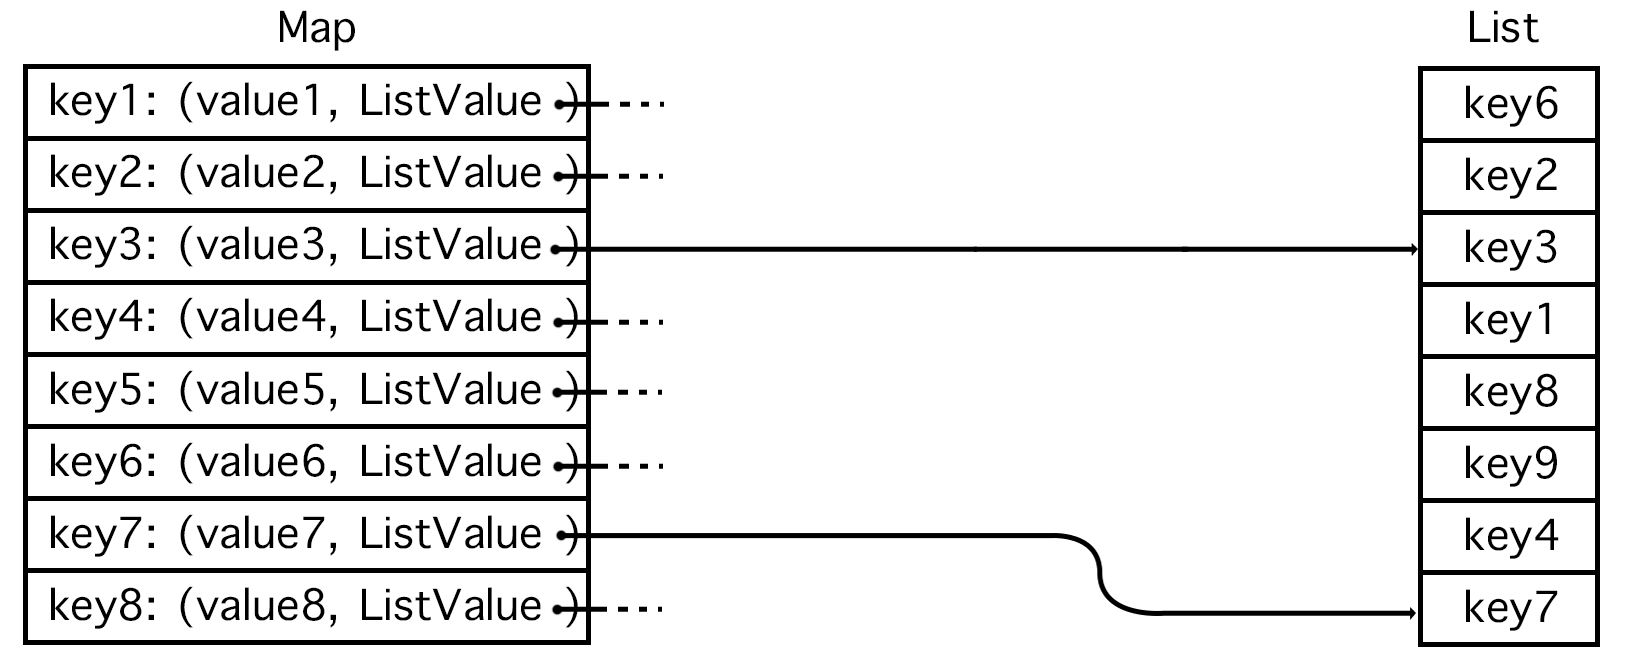
\includegraphics[width=\textwidth,height=\textheight,keepaspectratio]{img/lru.png}
  \caption{A visualization of the LRU}
  \label{fig:lru}
\end{figure}

\subsection{LRU warmup}\label{sec:warmup}
The main issue of using an LRU-style caching is that initially, the performance will be as bad as having no caching optimization at all. This is because until we actually have any previous calculation cached, we will still have to do all the calculations one by one. 

One possible solution for this is to employ a combination of the optimization that were presented. Since some of these optimizations work on different parts of the repartition process, we can actually use them together to have even better performance gains. For example, we can use the hot groups optimization, discarding the combinations of groups that are highly unlikely to be any good, and once we have the result we cache it in the LRU data structure. The hot groups approach would improve the performance of the system while the LRU is cold, and even when the LRU is warmed up the hot groups optimization would still be useful when we have a cache miss.

A possible flaw of this approach is that if one of our optimizations makes use of important approximations, then the values we store in our cache might be far from optimal; therefore, we have to be careful not to exaggerate with the approaches used. This could also be approached in a hybrid way; it is possible to use the approximation methods while the cache is empty, so that we speed up the first repartitions. Then, once the cache is full enough, we can start using the All-combinations method whenever we have a cache-miss, so that we can start using the optimal values without having a noticeable impact on the performance of the system.

Lastly, another alternative solution to manage the bad performance of a cold LRU is to pre-load the LRU. As long as the system remains the same, we know that the cached values will still be valid. Therefore we can either store the LRU data from a previous execution, so that we can reload it before the next one, or we can pre-compute some entries of the LRU before any execution, for example entries that we expect to be likely found in our application. This would greatly reduce the drawbacks of a slow start.

% \clearpage
\chapter{Optimizations experiments}\label{sec:optimizations-evaluation}
In this section we will test and compare all the different approaches to perform the repartition that were presented in the previous chapter.

In particular, we will be focusing on the time required to complete the repartition and on its quality. To assess the quality, we will first check how different the partitions assignments are (meaning, how differently the objects are assigned to the groups). Then we will compare the average cost and the standard deviation of the resulting partitioning. 

For each case, we will use an initially empty B+tree of maximum slot-use, or branching factor, equal to 100. We then have variables \texttt{ITEMS}, with possible values $100'000$, $500'000$ and $1'000'000$, and \texttt{GROUPS}, with values $3, 4, 8$. The graph structure used for the groups is symmetrical, with a latency of 100ms between all pairs of groups.

We start each test by inserting in the B+tree a number of new values equal to \texttt{ITEMS}, distributed on an interval from $0$ to \texttt{2$\cdot$ITEMS}. We then repartition, so that the RW counters get reset. This avoids that these initial inserts affect the RW counters of the repartition, altering the results. After this first repartition, we perform, for each group, \texttt{2$\cdot$ITEMS} operations, with a 50\% ratio of writes and reads. Each client has a distribution that follows a zipf distribution\cite{zipf} with $\alpha=0.5$. Also, the distribution is shifted for each group, by an amount depending on the number of groups. For example, if we have 3 groups and a range of 100 keys, for group 1 we will have a distribution centered at key 0, group 2 at key 33, and group 3 at key 67.

Finally we perform a second repartition, which will be timed to see fast the repartition algorithm is. Note that since we perform operations on the whole range of keys, it means that we will be repartitioning all the nodes at once, which is the quite rare worst-case performance.

For the last two test cases, the ones regarding the LRU caching, we perform the test differently, since it is a different type of performance optimization. We do the setup part of the test as before, but we perform the operation and repartition one hundred times instead of only once. This is because its usefulness only shows once we have performed multiple repartitions.

% [put picture that shows client loads/skews during tests]
% \begin{figure}[!htb]
%   \centering
%   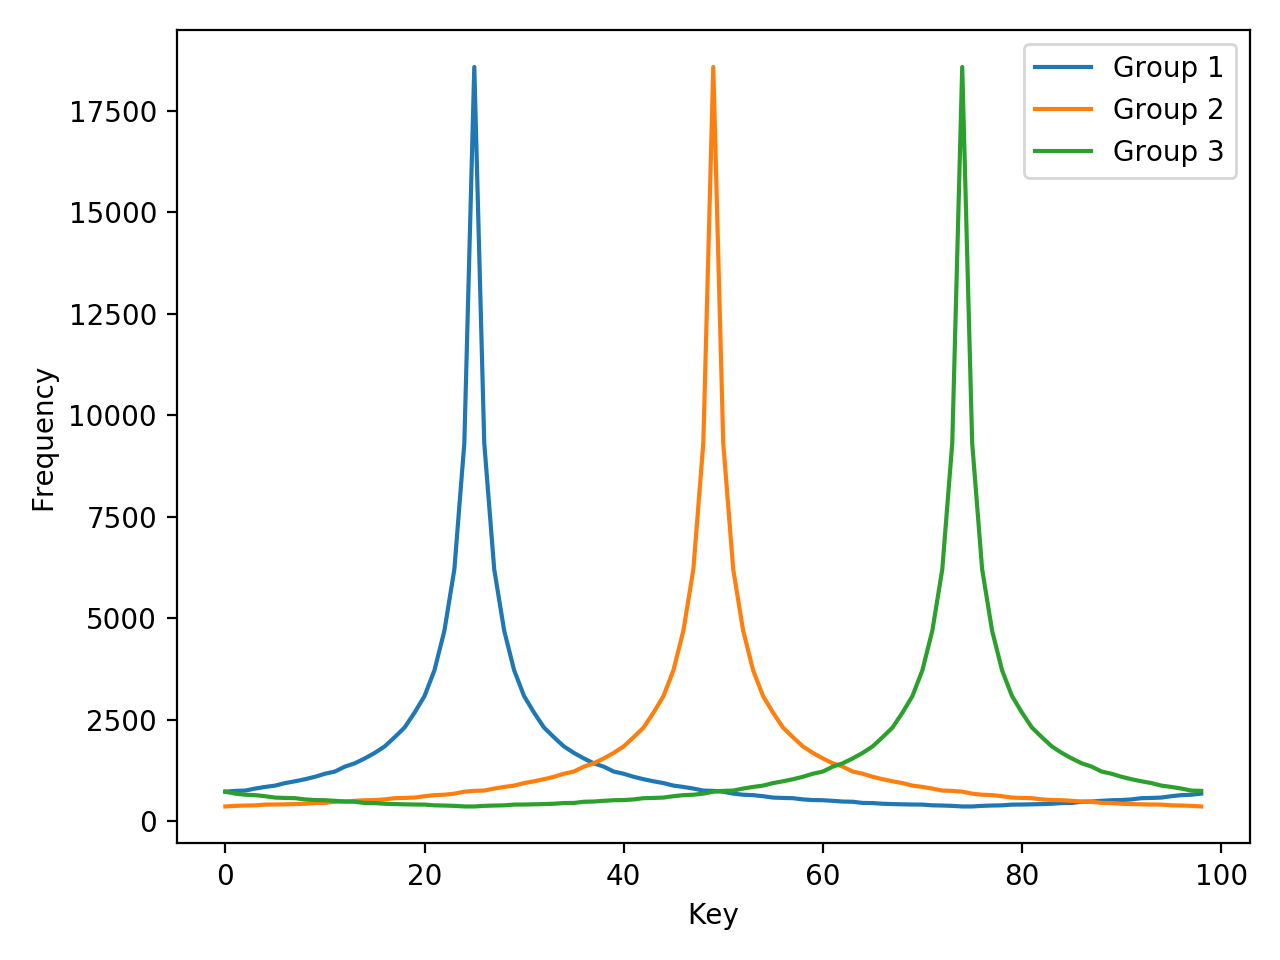
\includegraphics[width=\textwidth,height=\textheight,keepaspectratio]{img/clients_loads.png}
%   \caption{A visualization of the distribution of clients operations from the different groups and regions.}
%   \label{fig:all}
% \end{figure}

% \clearpage
\section{All-combinations experiments}\label{sec:All-combinations}
This scenario will be used as a baseline against which we will compare all the other algorithms. Since in this case we are considering all the possible combinations of node assignments, this algorithm will give us the best possible partitioning of a workload. At the same time it will also be the slowest one, which makes it not ideal considering that we would like to perform repartitions quite frequently, to make sure that the current partitioning matches the load of the system.

\begin{figure}[!htb]
  \centering
  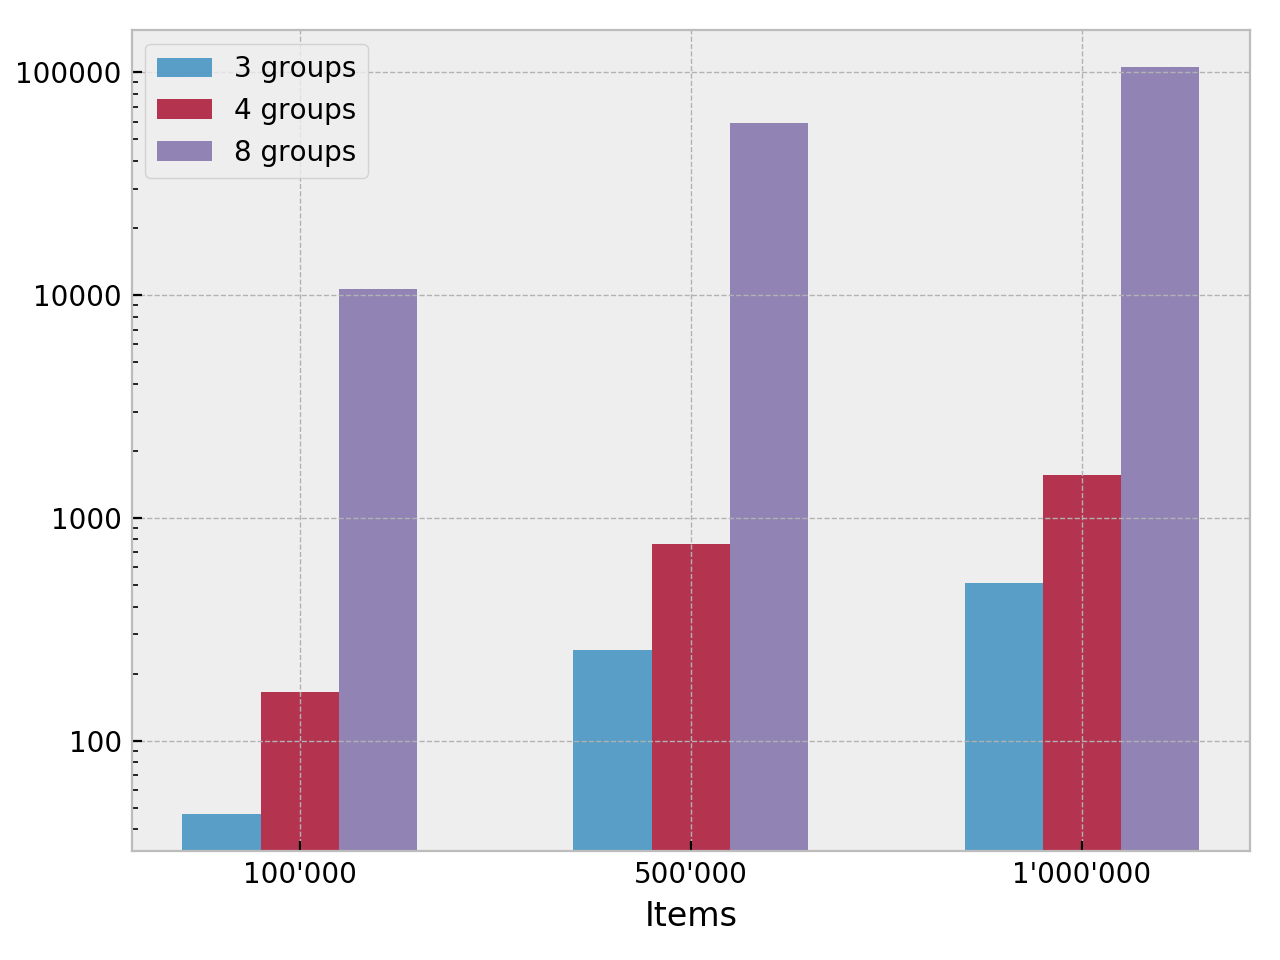
\includegraphics[width=\textwidth,height=\textheight,keepaspectratio]{img/all.png}
  \caption{The performance of the all-combinations method with different groups and items number}
  \label{fig:all}
\end{figure}

\subsubsection{Performance}
As we can see in Figure~\ref{fig:all}, the performance slows down linearly with the number of objects in the tree, and exponentially in the number of groups, as expected. The time required to perform a total repartition becomes quickly too big, even with a relatively small tree.

% \clearpage
\section{Fixed-size buckets experiments}\label{sec:fixed-size buckets-tests}
This approach groups the nodes in \emph{buckets} of size two, which means that the nodes of even levels of the tree will inherit the partitions of their parent node. This reduces the number of calculations of a factor of approximately $b$, the branching factor. Therefore, we expect the repartitions to take much less time compared to the previous approach. At the same time, we know that the partitions will be greatly approximated, since we will have all the leaf nodes, the ones containing the objects, approximating their partitions to the ones of their parent node.

\begin{figure}[!htb]
  \centering
  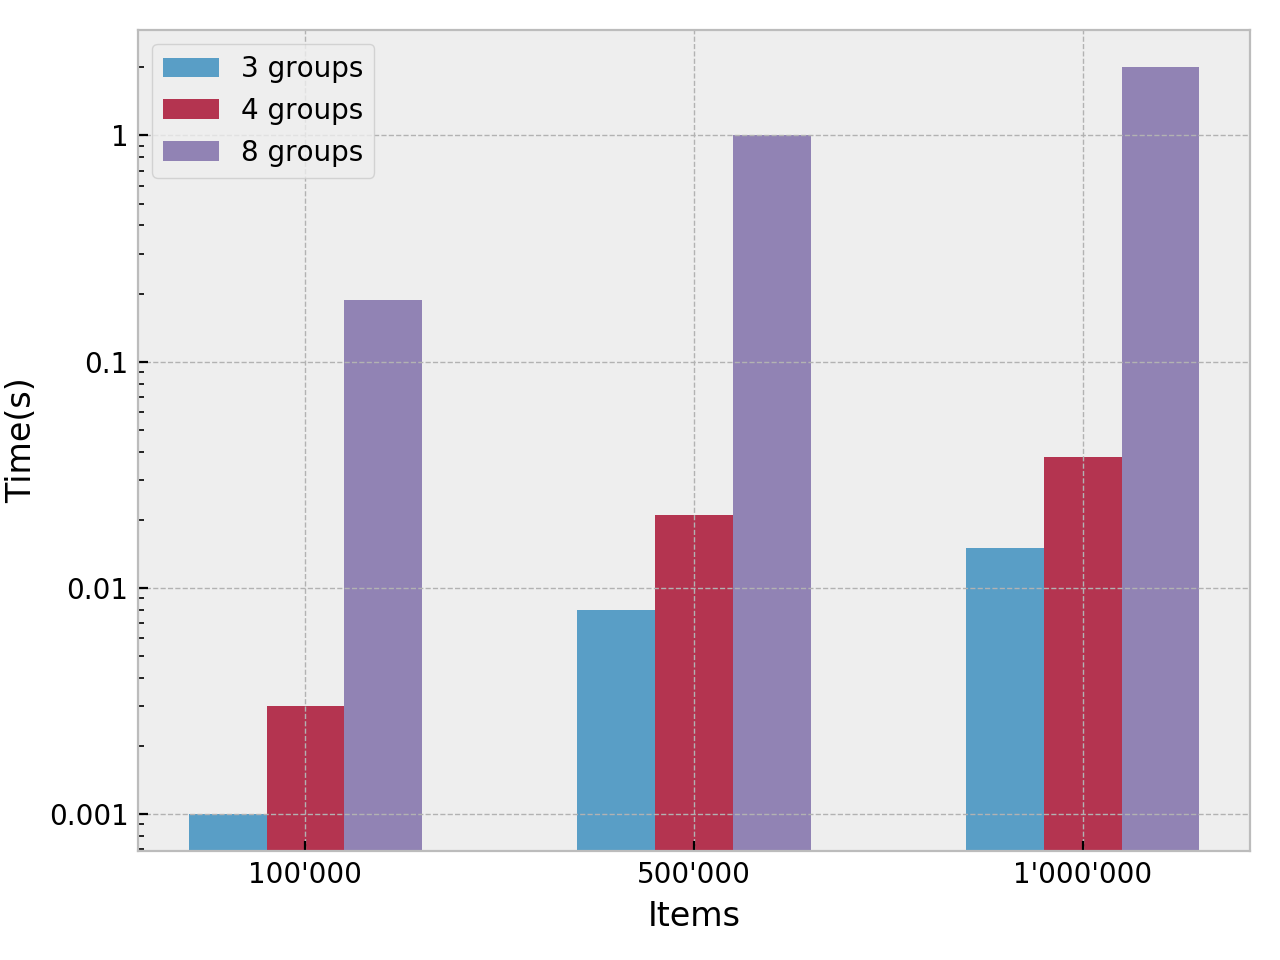
\includegraphics[width=\textwidth,height=\textheight,keepaspectratio]{img/fixed.png}
  \caption{The performance of the fixed-size buckets method with different groups and items number}
  \label{fig:fixed}
\end{figure}

\begin{figure}[!htb]
  \centering
  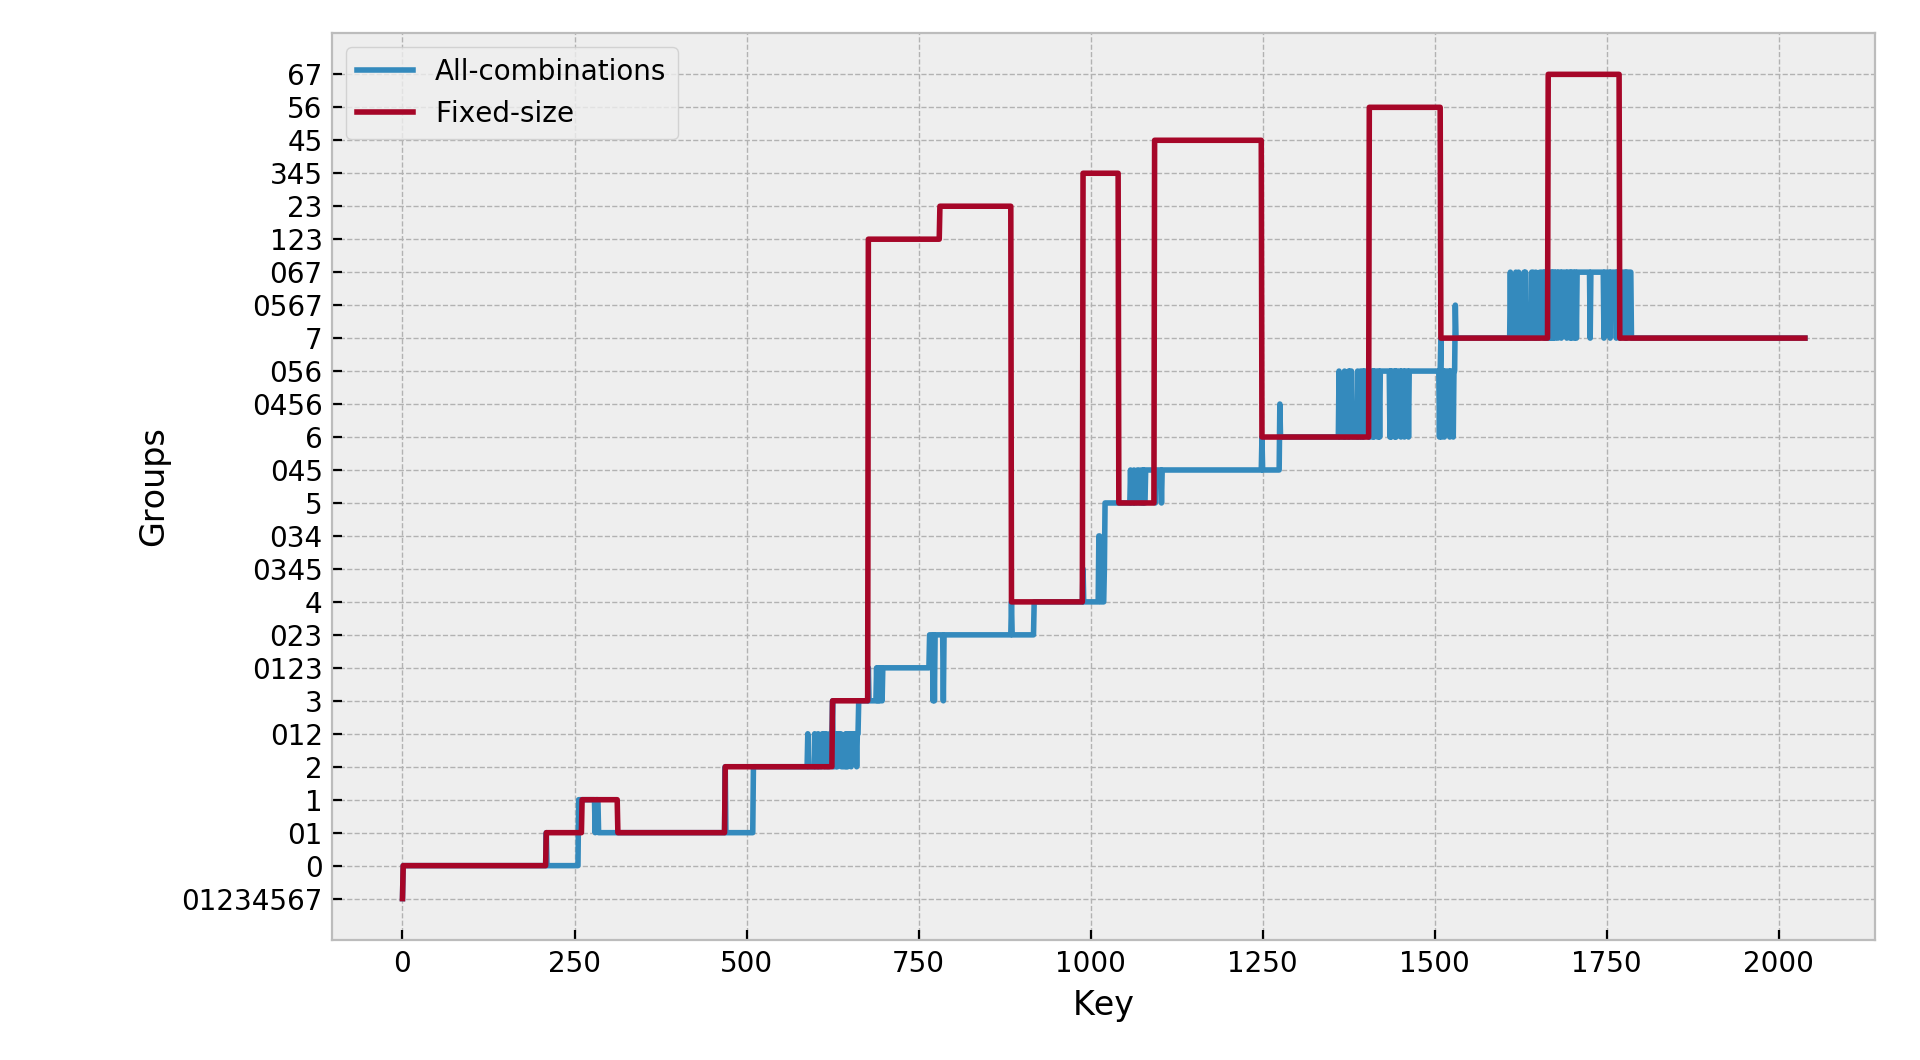
\includegraphics[width=\textwidth,height=\textheight,keepaspectratio]{img/partition_difference_fixed_all.png}
  \caption{The difference in group assignment between all-combinations and fixed-size}
  \label{fig:fixed-partitioning}
\end{figure}

\subsubsection{Results}
Figure \ref{fig:fixed} shows the results of the experiments. As expected, the time required to perform the repartitions is greatly reduced compared to the previous case. 

Figure \ref{fig:fixed-partitioning} shows a comparison between the group assignments of the objects after the repartition with the fixed-size and all-combinations methods; for each key (which represents an object in the tree) we can see which groups are assigned to be responsible for the ordering of operations. This specific experiment was done with 8 groups and a possible range of keys from 1 to 100'000. At the time of the repartition we had 2039 objects in the tree, and we have a total of 801 different assignments between the two approahces. A different assignment does not tell us how much it impacts performance, though; we have to check the actual latency costs for that.
To quantify the quality of this repartition, we calculate mean and standard deviation with the costs of the object assignments with the two methods. Table \ref{tab:mean-stddev-fixed-all} shows these statistics. As we can see, the mean cost for the fixed-size approach is around 30 times the cost of all-combinations, which sounds really bad. Furthermore, the standard deviation is twice as much, which still doesn't sound great. Given these results, the main reason to use this approach appears when the time of repartition is of much greater importance compared to its precision.

\begin{table}[!htb]
  \centering
  \begin{tabular}{l c c c}
    \hline
    & \textbf{Total cost} & \textbf{$\mu$} & \textbf{$\sigma$} \\
    \hline
    \textbf{All-combinations} & 53575400 & 26275.3 & 519570\\
    \textbf{Fixed-size} & 1547337300 & 758871 & 1057130 \\
    \hline
    \textbf{Ratio} & x28.8 & x28.8 & x2.03 \\
    \hline
  \end{tabular}
  \caption{Comparison of statistics between variable-size and all-combinations}\label{tab:mean-stddev-fixed-all}
\end{table}

% This becomes particularly apparent when we have many groups and many different loads. In the case with 8 groups and 100'000 items, out of 2039 nodes we have that 780 of those had different partitions assigned to them, which is more than one third wrongly approximated nodes. Given these results, the main reason to use this approach appears when the time of repartition is of much greater importance compared to its precision.

% \clearpage
\section{Variable-size buckets experiments}\label{sec:Variable-Size-buckets-tests}
This approach is slightly more refined compared to the fixed-size approach, therefore we expect to see slightly better results. Since this approach generally computes more calculations compared to the fixed-size, we would expect the timings to be worse than the previous approach but still better than the all-combinations one. We would also expect to see better partitions assignments. 

For this method, we also have to define a threshold value that is used to decide when it is worth computing the combinations for a node and when it is not. For our tests, we used as a threshold value $THRESHOLD = 0.8$, which means that if a node accounts for at least 80\% of the average expected workload of a single child node, then we will peform its calculations. There is no particular meaning behind the value we chose; we simply ran some tests and saw that it seemed to work quite well. Therefore, there is definitely room for further improvement. Still, it should be good enough to show the behavior of this approach.

\begin{figure}[!htb]
  \centering
  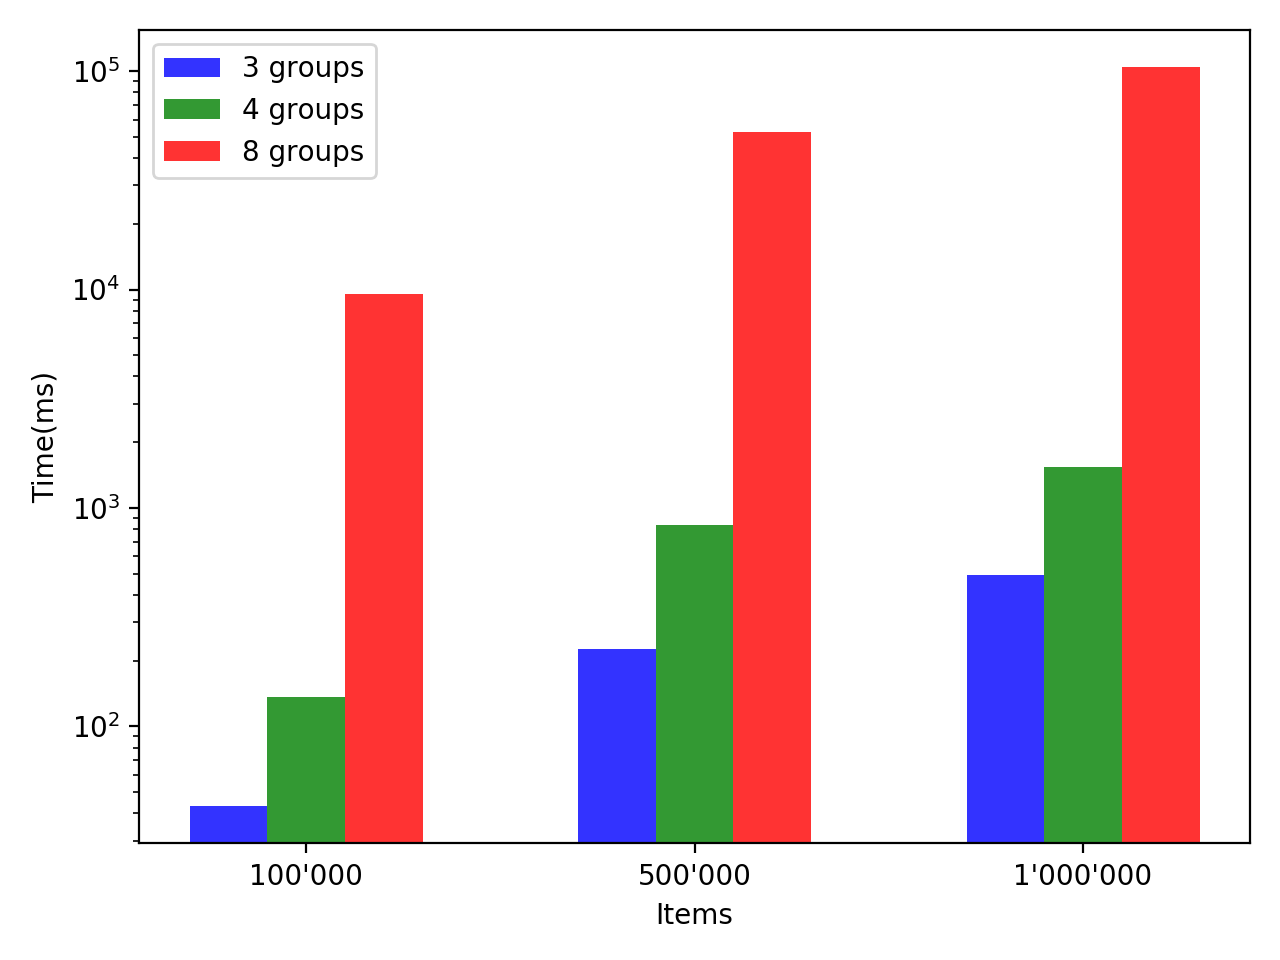
\includegraphics[width=\textwidth,height=\textheight,keepaspectratio]{img/dynamic.png}
  \caption{The performance of the variable-size Buckets method with different groups and items number}
  \label{fig:dynamic}
\end{figure}

\begin{figure}[!htb]
  \centering
  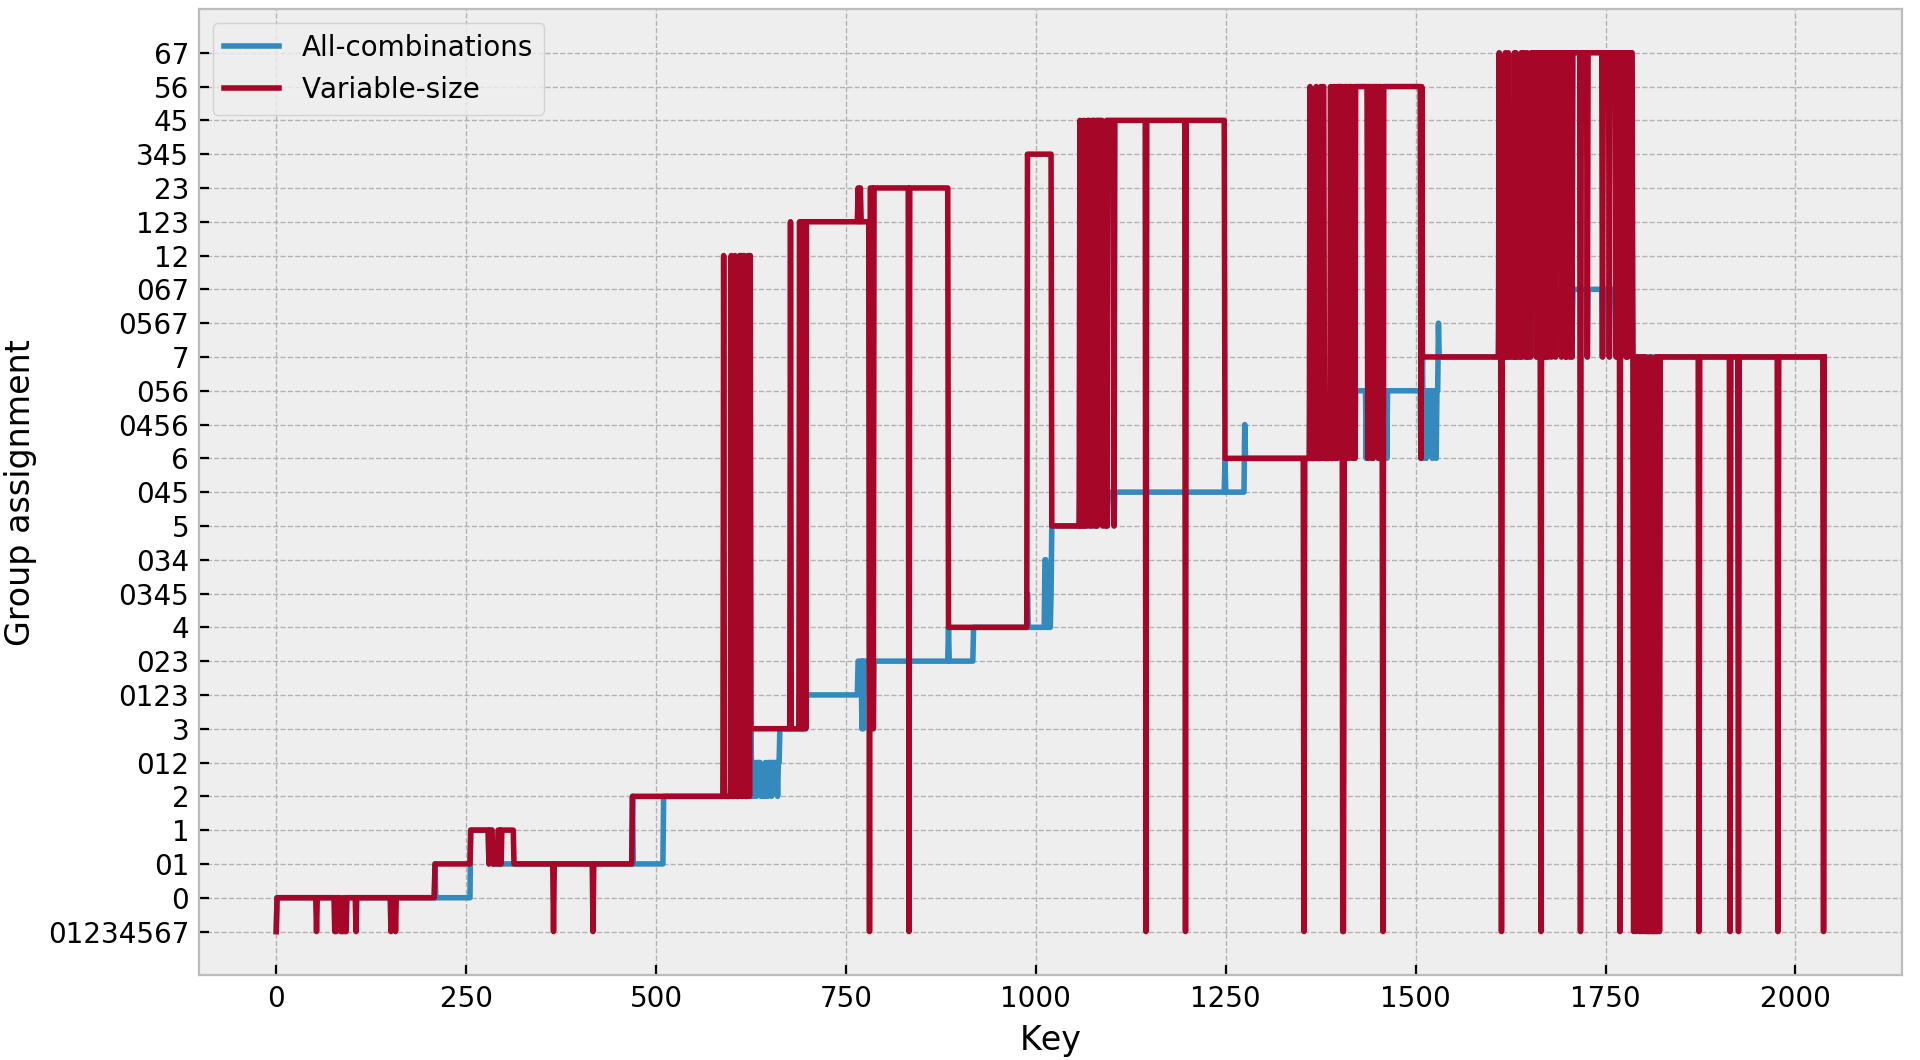
\includegraphics[width=\textwidth,height=\textheight,keepaspectratio]{img/partition_difference_variable_all.png}
  \caption{The difference in group assignment between all-combinations and variable-size}
  \label{fig:variable-partitioning}
\end{figure}

\subsubsection{Results}
Based on the results shown in Figure \ref{fig:dynamic}, this approach does not perform as well as expected: the performance is slightly better than the all-combinations approach, but not by far, and it is much slower than the fixed-bucket approach.

\begin{table}[!htb]
  \centering
  \begin{tabular}{l c c c}
    \hline
    & \textbf{Total cost} & \textbf{$\mu$} & \textbf{$\sigma$} \\
    \hline
    \textbf{All-combinations} & 53575400 & 26275.3 & 519570\\
    \textbf{Variable-size} & 427262400 & 209545 & 1043720 \\
    \hline
    \textbf{Ratio} & x7.97 & x7.97 & x2.01 \\
    \hline
  \end{tabular}
  \caption{Comparison of statistics between variable-size and all-combinations}\label{tab:mean-stddev-variable-all}
\end{table}

As we previously did for the fixed-size experiments, we then took the test with 8 groups, 100'000 maximum items and we checked the number of different partition assignments (See figure \ref{fig:variable-partitioning}). The total number of different partition assignments is similar, 818 differences out of 2039 objects. This is even more differences than in the fixed-size experiments, but we first have to check the mean and standard deviation before drawing conclusions.

In Table \ref{tab:mean-stddev-variable-all} we can see the statistics regarding the variable-size method. The mean is particularly improved, being around 8 times more than the all-combinations and 3.6 times less than the fixed-size mean. The standard deviation is really similar to the fixed-size, so no particular improvement on that side.
Looking back at the plot of Figure \ref{fig:variable-partitioning}, we can also guess why the results are so bad: there is quite a big amount of nodes that inherited the partitions from their parents recursively, ending up with objects with the same group assignments as the root. 

This method definitely performs less approximations compared to the fixed-size approach, but the difference in the time required for the repartition makes the variable-size approach really hard to recommend for any use. Still, We believe that this method could perform better if we improved the way used to choose which nodes to calculate.

% \clearpage
\section{Hot groups experiments}\label{sec:hot-groups-experiments}
The hot groups approach aims at discarding combinations of groups, rather than nodes like the previous methods. This means that we expect to see an increasing gain in performance once we increase the number of groups, rather than the number of items.

In general we expect this method to perform similar to the all-combinations one in the case with few groups, but we should also have a much more linear increment in time with the tests with more groups. We should also get better partition assignments compared to the bucket approaches, since we expect the heuristic of discarding groups to give us better results than the ones used previously.

Like in the variable-buckets case, we have a threshold variable to set. This time it is used to decide if we should discard a group or not. We set the variable to $0.1$, which means that if a group has less than 10\% the RW counters of the group with the most RW counters of this node, then we will discard it. It is important to notice that the partitions assignment also depends on the ratio of reads and writes. We could use more complicate ways to calculate the threshold, taking into account the read/write ratio as well, but we preferred to keep the number of variables as little as possible to avoid complicating the tests.

\begin{figure}[!htb]
  \centering
  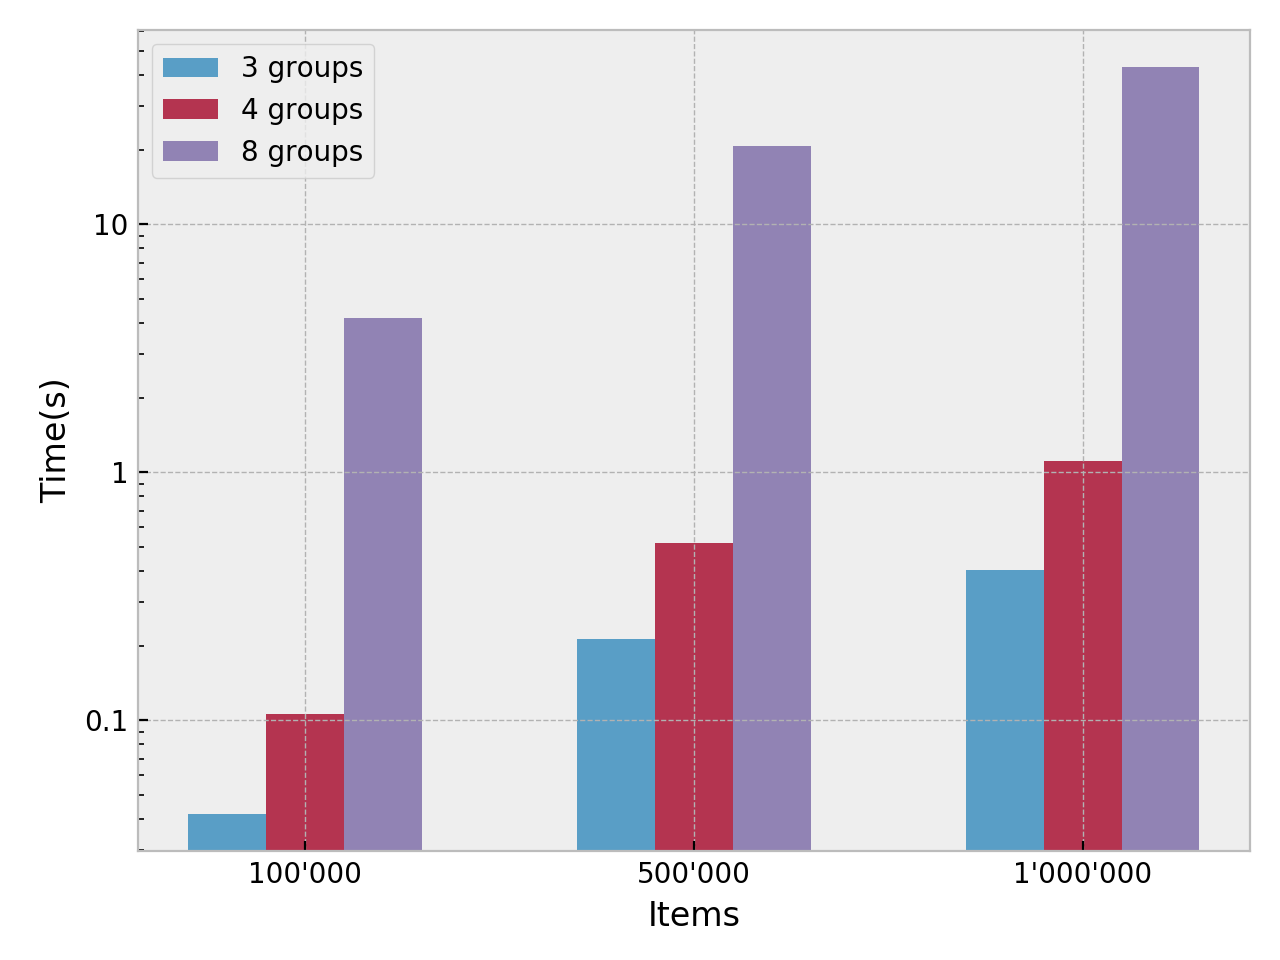
\includegraphics[width=\textwidth,height=\textheight,keepaspectratio]{img/hot.png}
  \caption{The performance of the hot groups method with different groups and items number}
  \label{fig:hot}
\end{figure}

\begin{figure}[!htb]
  \centering
  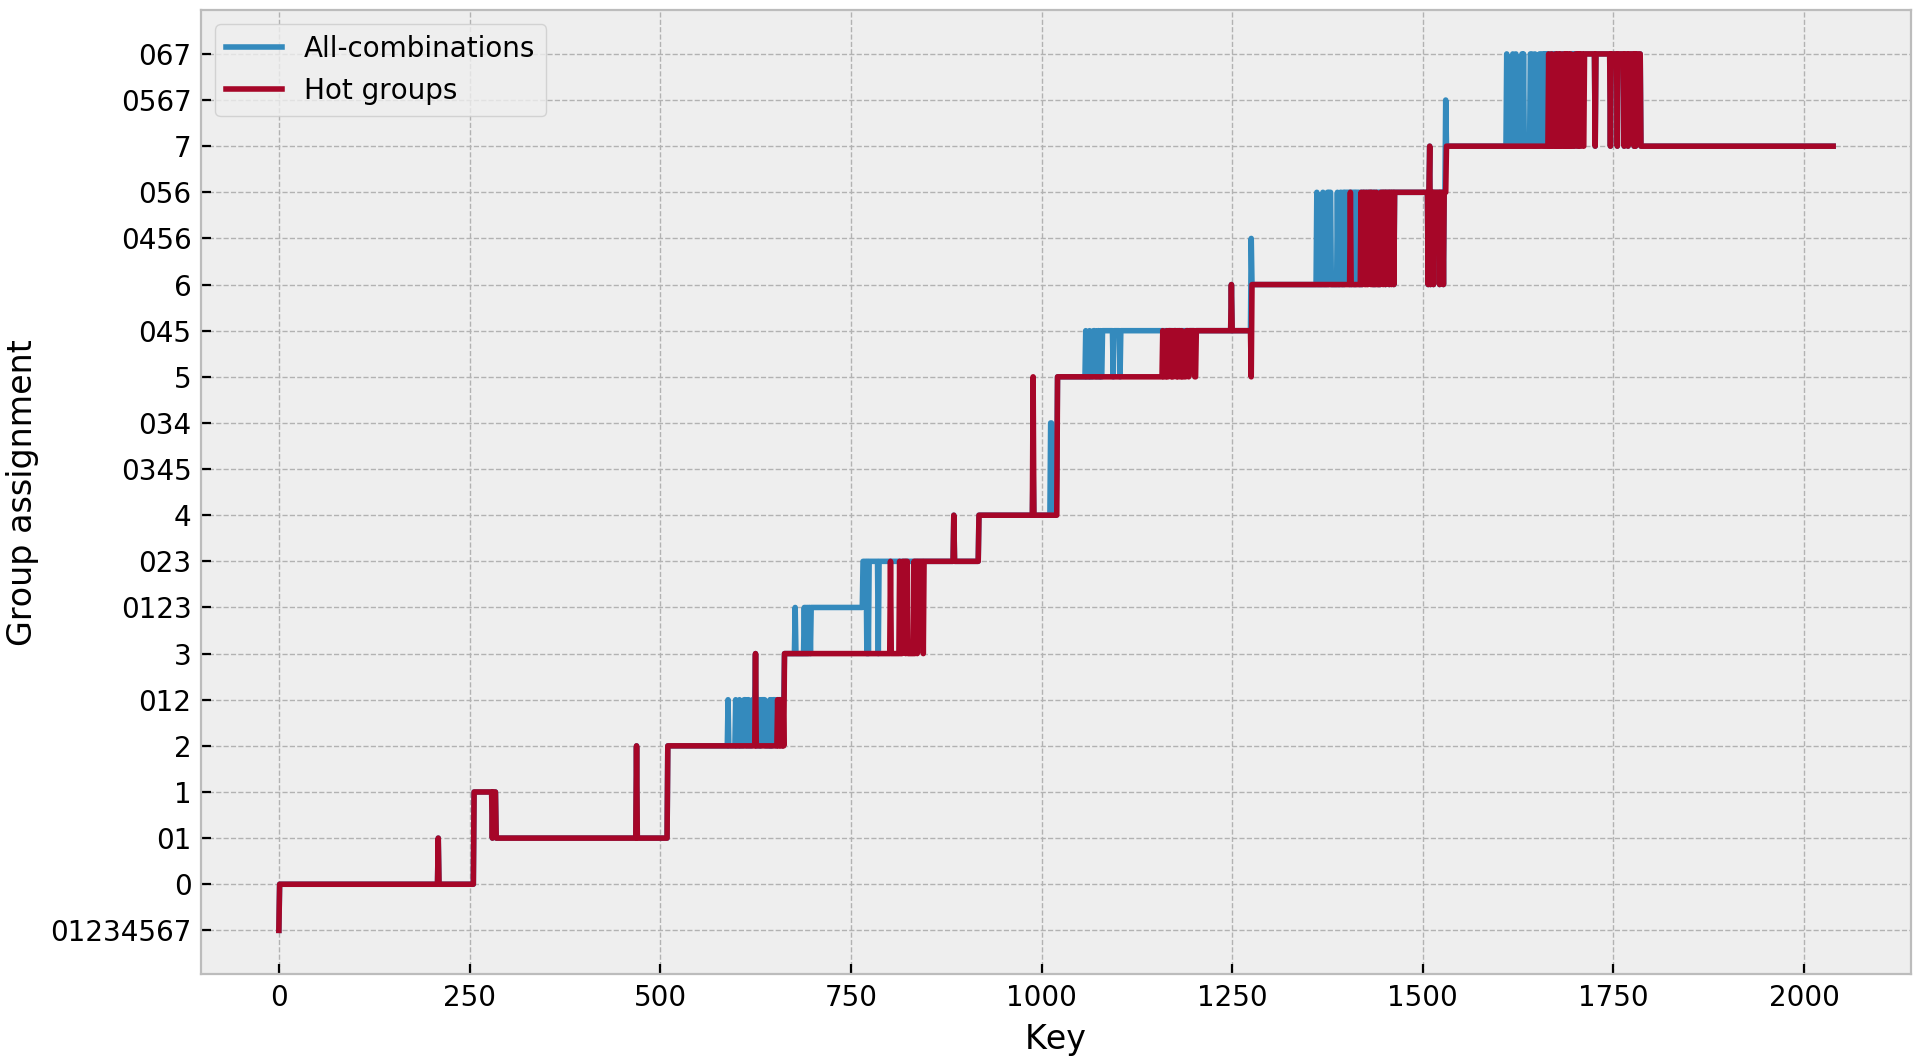
\includegraphics[width=\textwidth,height=\textheight,keepaspectratio]{img/partition_difference_hot_all.png}
  \caption{The difference in group assignment between all-combinations and hot groups}
  \label{fig:hot-partitioning}
\end{figure}

\subsubsection{Results}
In this case, the results of the experiments shown in Figure \ref{alg:hot-groups} are as expected. When compared to the all-combinations case, we see that the performance in the tests with 3 groups are very similar, with the hot groups approach taking around 10-20\% less time. When we move onto 4 and 8 groups though the improvement is definitely more noticeable, with improvements in the order of 30-40\% and up to 65\% respectively.

Regarding the precision of the repartition, shown in Figure \ref{fig:hot-partitioning}, we see a difference of 380 out of 2039 nodes in the test with 100'000 items and 8 groups.
The differences are mostly in the number of partitions that the nodes are assigned to. The all-combinations approach assigns the nodes to multiple partitions more often than the hot groups. This is because hot groups discards the groups with few operations, therefore not considering the partitionings with multiple groups.

The number of different partition assignments is around half of what we had with the previous methods, but this does not tell the whole story. If we look at the mean and standard deviation in Table \ref{tab:mean-stddev-hot-all} we see that the cost of the hot-groups method is really close to the all-combinations one, with a difference in mean of 2\% and in standard deviation of less than 0.1\%.

\begin{table}[!htb]
  \centering
  \begin{tabular}{l c c c}
    \hline
    & \textbf{Total cost} & \textbf{$\mu$} & \textbf{$\sigma$} \\
    \hline
    \textbf{All-combinations} & 53575400 & 26275.3 & 519570\\
    \textbf{Hot groups} & 54724700 & 26839 & 519916 \\
    \hline
    \textbf{Ratio} & x1.02 & x1.02 & x1.00 \\
  \end{tabular}
  \caption{Comparison of statistics between hot groups and all-combinations}\label{tab:mean-stddev-hot-all}
\end{table}

% \clearpage
\section{LRU Caching experiments}\label{sec:lru-caching-tests}
As we said before, the Least Recently Used approach can be used with all the previous methods. For these tests, we will use it with the all-combinations approach, to see how much we can improve upon the algorithm that gives us the optimal repartitioning. Again, since the LRU performs well once the cache is filled, this test will be performed with a series of 100 repartitions, calculating the time for each of them.

For this test, we decided to use a cache size of 1'000'000. Obviously a bigger cache would further allow improvements on the performance, at the cost of an increased load on the memory. With this cache size, we reached a usage of approximately 450MB.

We do not have a clear idea of how much the LRU will improve the results. It is hard to say if the limited size of the cache will be the bottleneck that will impede further improvements, or if we will get to the point where the mandatory calculations will become the main bottleneck.

\begin{figure}[!htb]
  \centering
  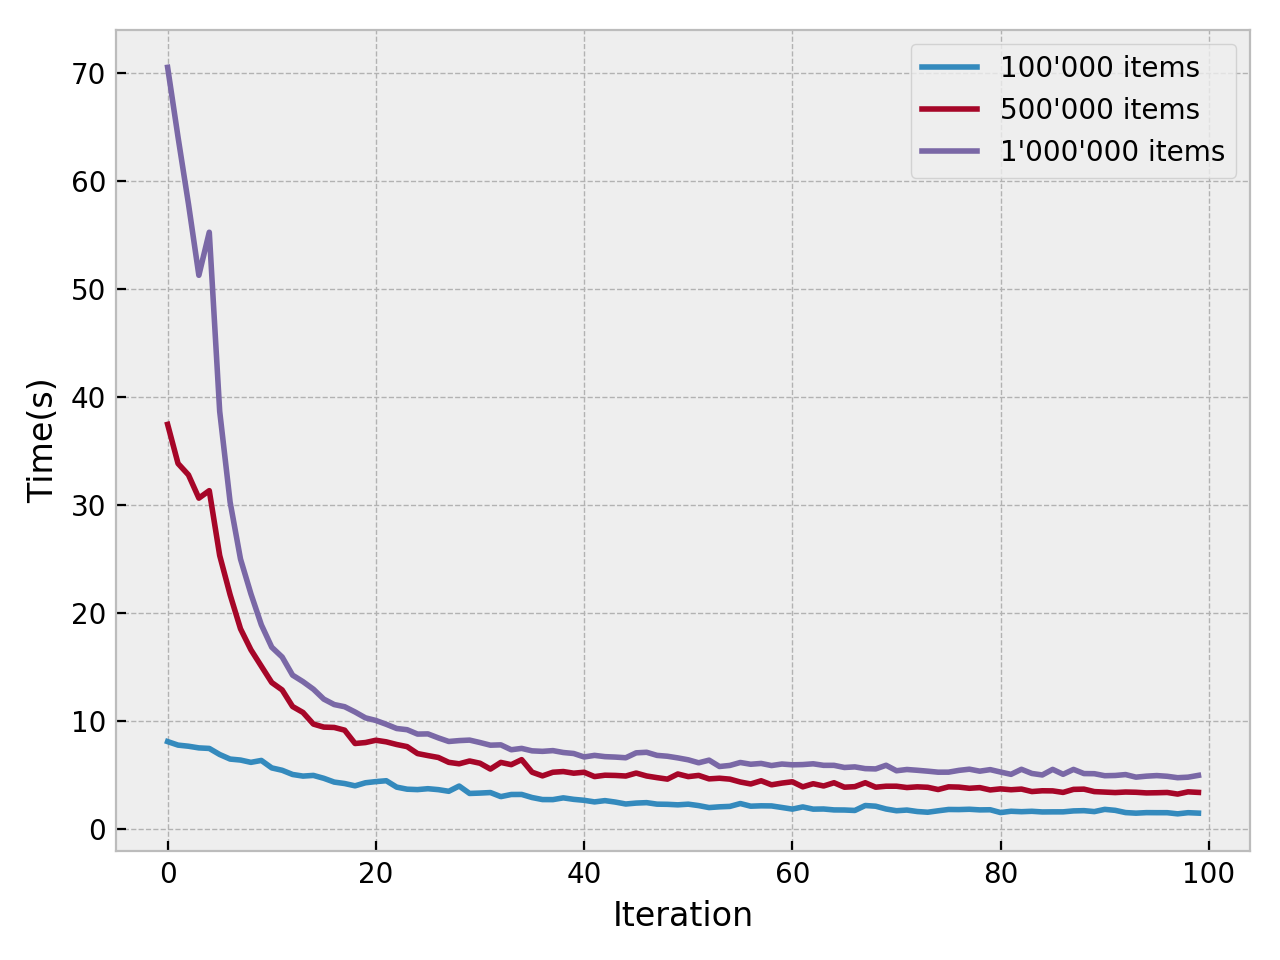
\includegraphics[width=\textwidth,height=\textheight,keepaspectratio]{img/LRU_8.png}
  \caption{The time required for 100 subsequent repartitions using the LRU and the all-combinations method }
  \label{fig:LRU_8}
\end{figure}

\subsubsection{Results}
Figure \ref{fig:LRU_8} shows the results of the experiments. The first impression is positive: in 100 repartitions the computation time decreased to one tenth of what it was initially, going below 10 seconds in the best cases. While 10 seconds is still a noticeable amount of time, with more repartitions the performance will increase even more. 

It is also interesting to notice that even in the first repartition, the time was around 70 seconds, definitely less than the 105 of the approach with LRU. This shows that even with just one repartition we have a noticeable amount of cache-hits. This most likely happens with close objects, that have a high chance of having similar workloads thanks to their high locality.
\\\\
To make sure that this approach still behaves as expected with other settings, we decided to also perform this test with a varying number of groups (3 and 4) and then with different distributions (with $\alpha =0$ and $\alpha =1$, meaning more flat and more steep, respectively). All of these tests were still performed with $1'000'000$ items. The results can be seen in Figure \ref{fig:LRU_8_extra}.
\\\\
The results are not surprising: the tests with fewer groups are much faster, but the shape of the plots is similar. The test with the different distributions are quite similar, with the performance being slightly higher when the distribution is flatter. This makes sense, since with a flatter distribution we have a higher chance of having similar workloads and therefore we would use the cached values more often.

\begin{figure}[!htb]
  \centering
  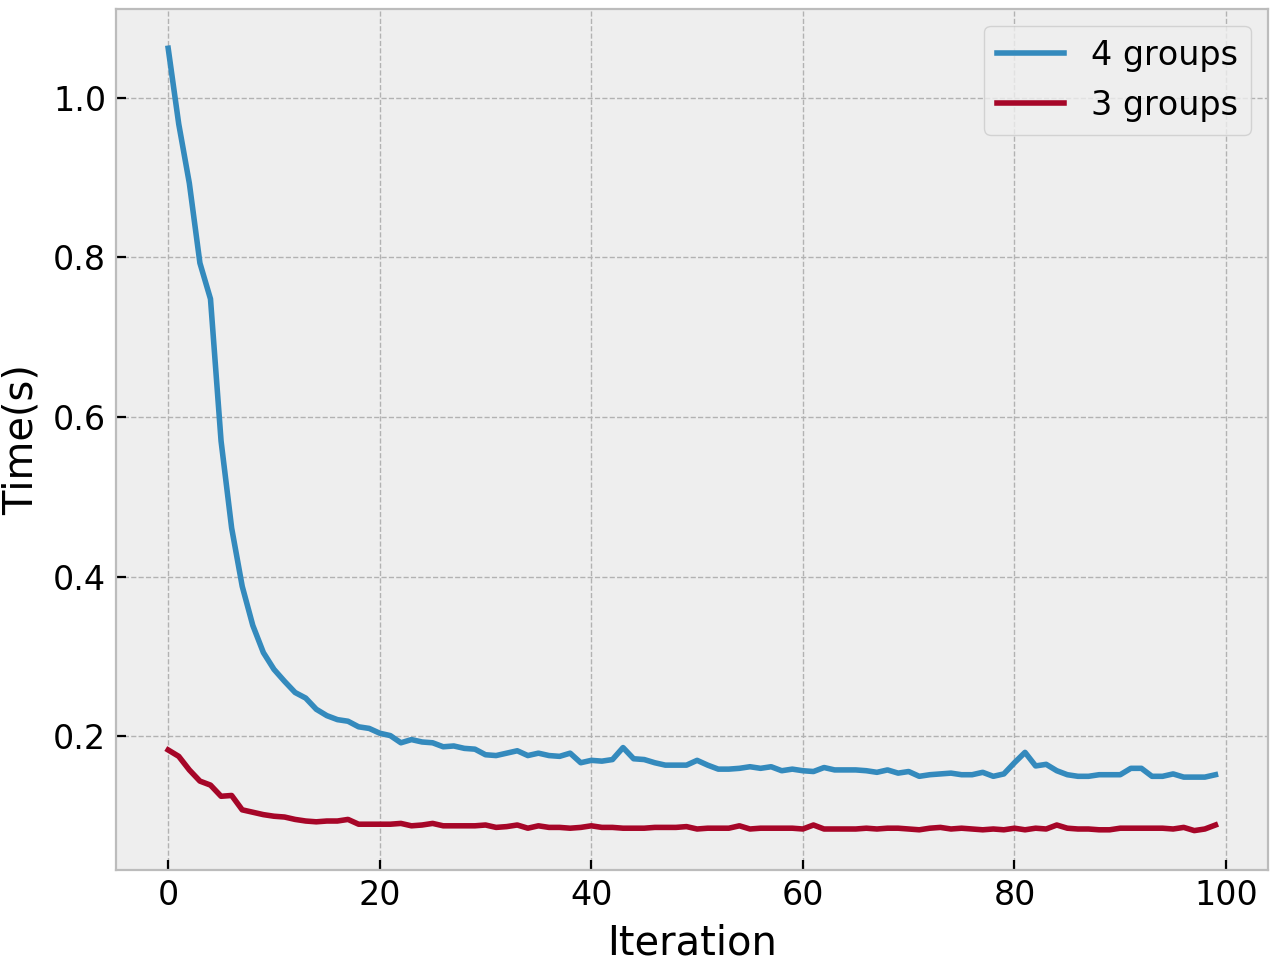
\includegraphics[width=0.49\textwidth,height=\textheight,keepaspectratio]{img/LRU_8_groups.png}
  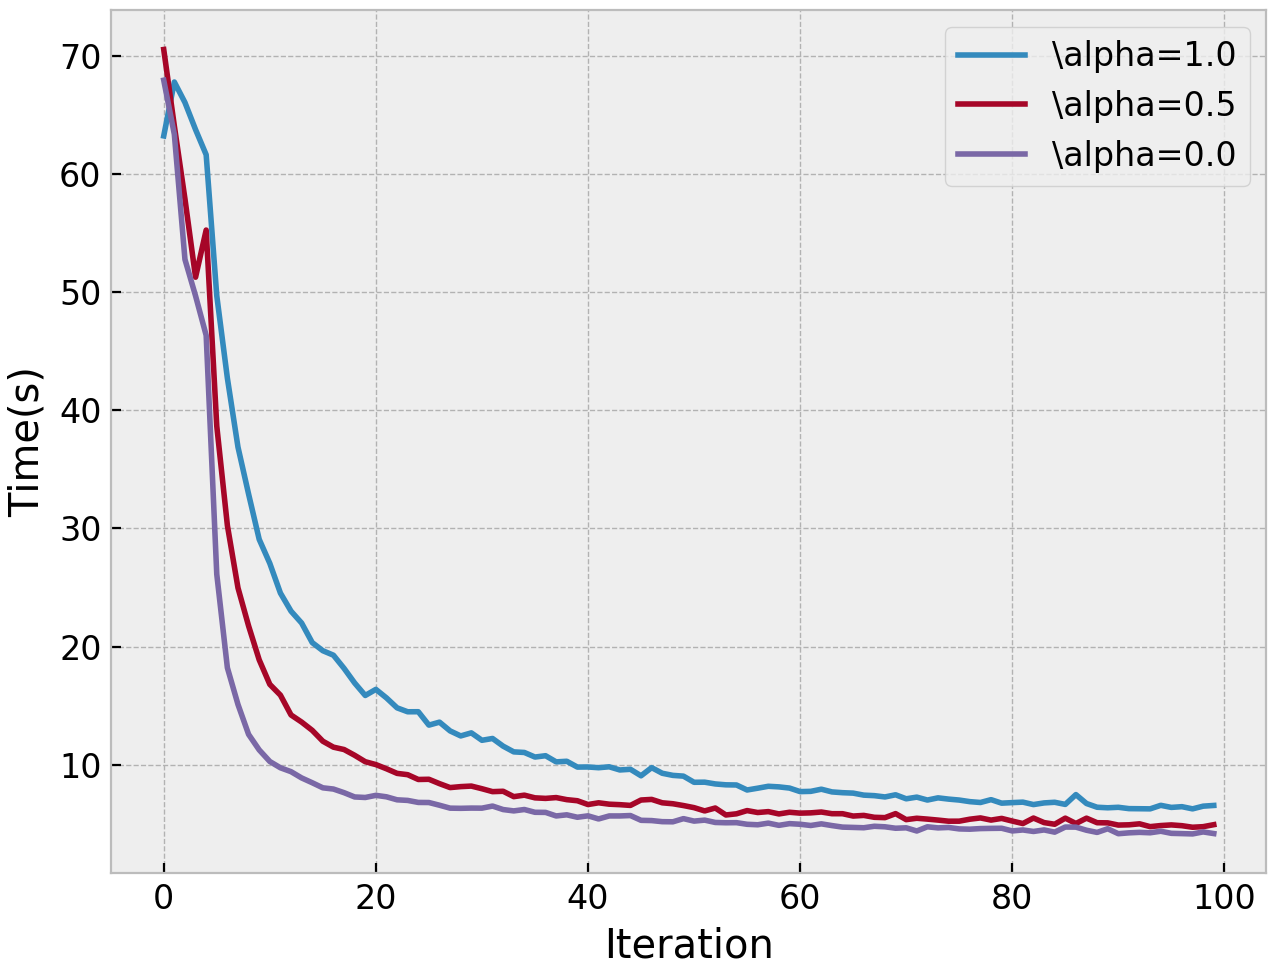
\includegraphics[width=0.49\textwidth,height=\textheight,keepaspectratio]{img/LRU_8_dist.png}
  \caption{ The results of the LRU test performed with different settings }
  \label{fig:LRU_8_extra}
\end{figure}


% \clearpage
\section{LRU with hot groups}\label{sec:lru-hot-groups}
We will now test the performance of the LRU combined with the hot groups approach. The idea is that the hot groups will make up for the slow initial repartitions when the LRU cache is empty. Once the cache is filling up the performance should increase rapidly, giving us good approximations of the repartitions thanks to the hot groups. 

\begin{figure}[!htb]
  \centering
  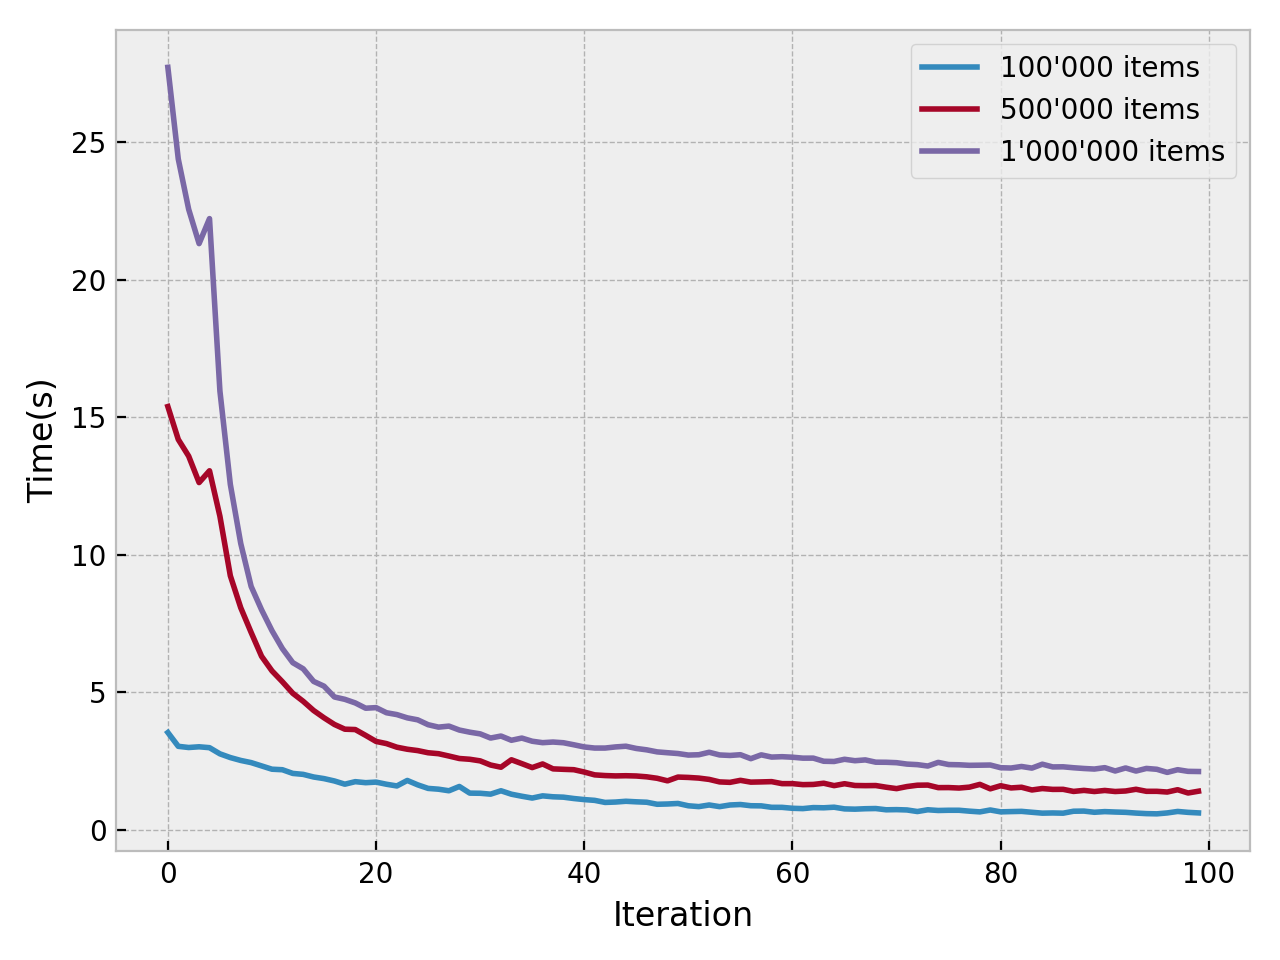
\includegraphics[width=\textwidth,height=\textheight,keepaspectratio]{img/LRU_8_hot.png}
  \caption{The time required for 100 subsequent repartitions using the LRU and the hot groups method}
  \label{fig:LRU_8_hot}
\end{figure}

\subsubsection{Results}
The results shown in Figure \ref{fig:LRU_8_hot} are in line with our expectations. The shape of the plots is similar to the one with all-combinations, but all the curves are lower, which means that this approach always takes less time than the previous one, at the cost of precision. The percentage decrease in computation time is similar to the percentage decrease we saw when comparing all-combinations and hot groups without the LRU. 

% \clearpage
\section{Repartition results evaluation}\label{sec:repartition-results-evaluation}
Based on the results, we can draw some conclusions on the quality of the various methods compared against each other. 
\\\\
The all-combinations approach gives us the optimal partition assignments to obtain minimum average latency, but in the case of a repartition of relevant size the time it takes is definitely too long. the combinations with 8 groups take from 10.5 to 105 seconds; it might not be possible to stop execution for that long, unless we perform repartitions very infrequently.
\\\\
The fixed-size buckets approach is on the other end of the spectrum; really short computation times, but it leads to great approximations in the repartition. Still, with 8 groups, 1 million items workload, the repartition time was 2 seconds compared to 105, so it looks at least usable as a starting approach or when timing is a great concern.
\\\\
The variable-size buckets turned out to be rather disappointing. Computation times are slightly better than the all-combinations approach, but an average cost and standard deviation which are not much better than the fixed-size method. perhaps it was a bad test case for this method; different loads and different tresholds may lead to better results. Yet, we cannot feel encouraged to use this method given the results we have at hand.
\\\\
The last computation optimization, the hot groups, performed quite well. In particular, the computational times with 8 groups are less than half compared to the all-combinations, which is a nice improvement, and the number of wrong assignments is half of the fixed-size buckets, with average and standard deviation costs very clsoe to the all-combinations approach. In general, it looks like the most balanced optimization. This method is also particularly useful because it targets the number of group combinations, which quickly becomes an issue because of its exponential growth.
\\\\
The results get particularly interesting when paired with the caching system. Even with the slowest computation method, the biggest workload goes from 105 seconds to less than 10 seconds in just 100 repartitions. When paired with a faster computation method, like hot groups, it goes even below 3 seconds. As a matter of fact, out of curiosity we tried with 1000 repartitions, and at the 500th one the time was around 1 second, plateauing at around 600, with around 950ms on average, and a memory usage of 1GB.
By comparison, the one without hot groups reached a plateau at 400 repartitions, with an approximate time of 2-2.5 seconds per repartition.

In conclusion, it looks like the way to go is definitely by exploiting the LRU caching, and pairing it with a different computational method depending on how time and precision are important for our system.

% \clearpage
\chapter{GeoPaxos experiments}\label{sec:geopaxos-tests}
Now that we have evaluated the performance of the various approaches, we will run a suite of tests with various types of settings, to simulate how the B+tree on top of GeoPaxos behaves in different situations.

\section{Tests setup}\label{sec:tests-setup}
It is quite hard to come up with tests that give us realistic workloads, but we believe that the tests we discuss in this section should give a decent idea of the cases where the repartition performs well and the cases where it could be improved. While we could have included more combinations of tests in the report, we believe that it would have become overwhelming and more confusing rather than adding any useful extra information.
\\\\
The tests have a range of variables to be set, including:
\begin{itemize}
  \item \textbf{Number of clients (per destination group)} The number of clients that are connected to each group of the system, e.g., the number of clients for each region.
  \item \textbf{Number of threads (per client)} The number of threads used for each client. Increasing the number of threads boosts the maximum throughput of a single client, but each client still has to receive a reply to a previous message sent before sending a new one. During testing we keep the value in a way so that the performance of the clients is consistent, and we use a high number of threads to limit the bottleneck of message handling so that we can focus the performance on the latency of communications.
  \item \textbf{Number of outstanding messages} The maximum number of requests that a client can have on-hold at once. If set to one, a client can only send a second request after it has received an answer for the first request.
  \item \textbf{Number of items} The total number of items, or keys, on which the clients can perform operations.
  \item \textbf{Maximum throughput (msgs/s)} The maximum number of messages that a client can send in a second.
  \item \textbf{Range of operations} The interval of keys that the client will perform operations on. This usually corresponds to the total number of items, but the beginning and end of the range will be shifted depending on the region of the client.
  \item \textbf{Ratio of operations} The ratio of read and write operations performed by the client.
  \item \textbf{Skew alpha} The skew of the zipf function that defines the frequency of operations on the range of keys (see Figure ~\ref{fig:skews}).
\end{itemize}
All the clients behave in the same way. Once started, they send messages to the replica that they are connected to (at a rate depending on the variables defined above), and waits for the replies.
\\\\
There are some possible behaviors of clients that may not seem important at first, but that are quite important to keep under control to avoid unexpected or unwanted results from the tests.

One interesting case happens when a client, because of a time period with a high throughput, has a repartition that puts a lot of objects in the region where he is. This leads to his operations having even lower latency than before, which leads to even higher throughput than before, leading to a situation where he will be the most efficient client exactly because it was efficient in the past. To handle this, we have two variables: the maximum throughput, that makes it so that after a certain point, the client cannot send more messages than a certain threshold.

Furthermore, we can increase the number of outstanding messages; while this sounds counterintuitive, having a higher outstanding limit allows slower clients to send more messages without having to wait for replies of past messages, limiting the gap between fast and slow clients.

Both these settings (maximum throughput and outstanding messages) could be realistic behaviours, too: common clients may not have the fastest internet speed, therefore limiting their maximum throughput, and not all requests may be dependent on each other, therefore a client will not have to wait a reply for all messages before sending new ones.
\\\\
The tests will proceed as follows. After having started all the replicas, we will start all the clients at the same time. We will perform the first repartition after 1 minute, since the system will initially be slow and without any previous RW counters to use. After that first repartition, we will perform further repartitions every 30 seconds. Every test will run for a total of approximately 5 minutes, during which 8 repartitions will be performed.

For each region, we will have 10 clients (with multiple threads for each client, to make sure that we maximize performance), with the distribution of operations dependant on the test. The clients will also have a limited throughput set to 50 messages per second. While this limits the maximum throughput of the system, it is important to remember that we do not want to test the maximum throughput, but only minimize the average latency. Furthermore, limiting the throughput simulates clients that do not have high speed connections, and it also avoids that just a few clients monopolize the system, giving all clients a fair opportunity to use the system.

\begin{figure}[!htb]
  \centering
  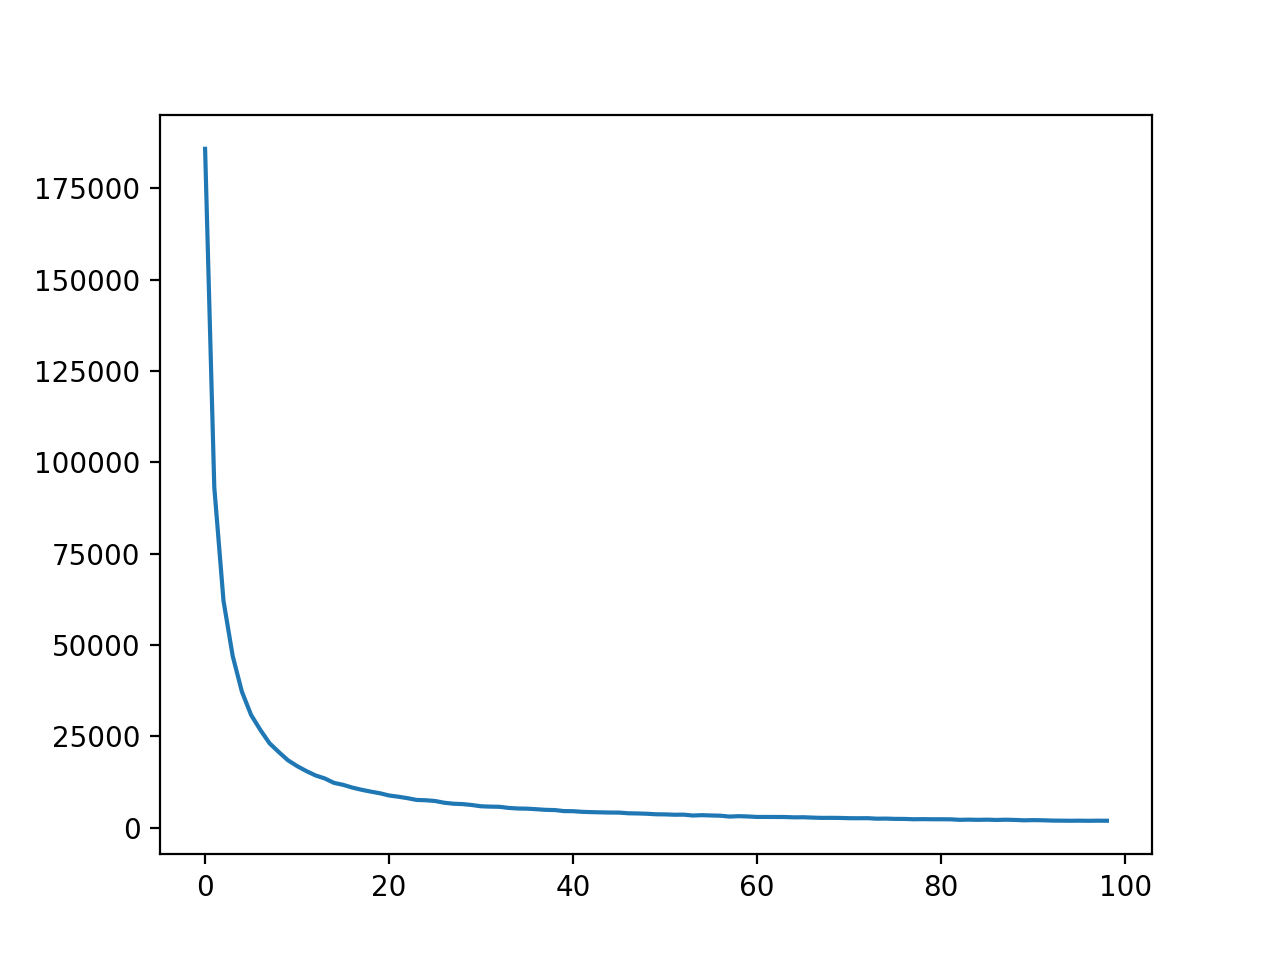
\includegraphics[width=0.49\textwidth,height=\textheight,keepaspectratio]{img/skew-alpha1.png}
  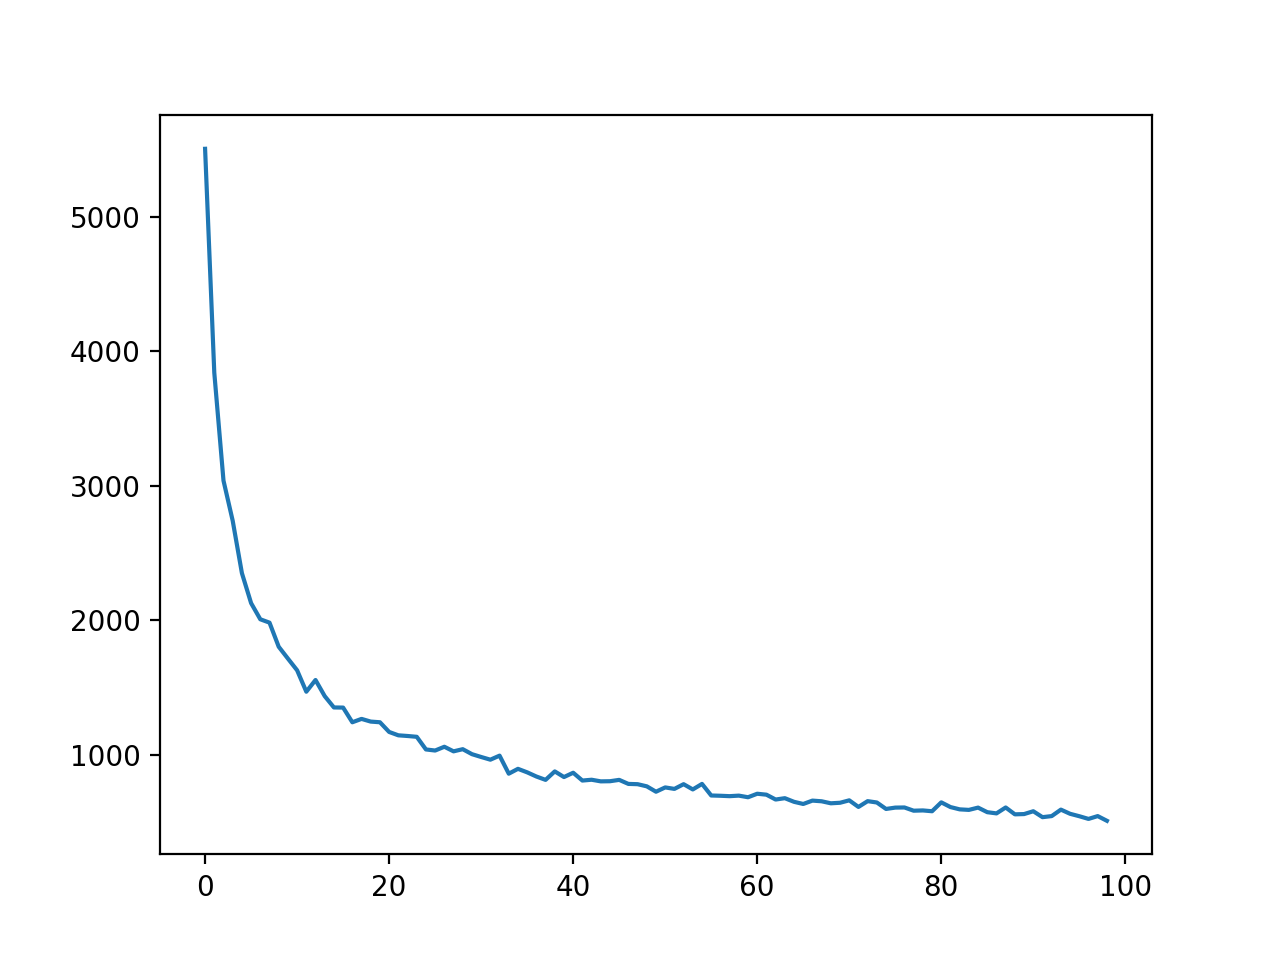
\includegraphics[width=0.49\textwidth,height=\textheight,keepaspectratio]{img/skew-alpha05.png}
  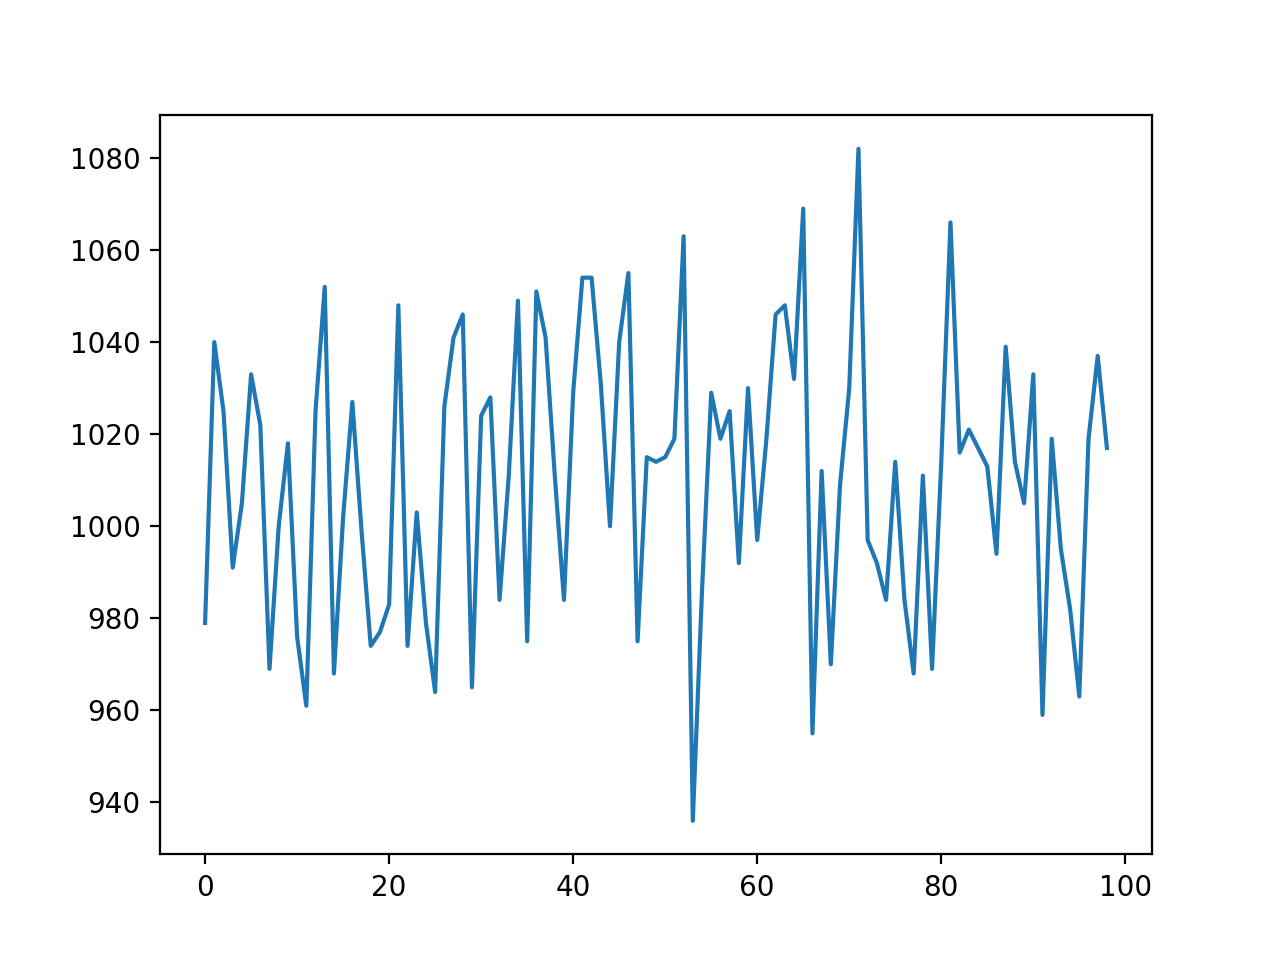
\includegraphics[width=0.49\textwidth,height=\textheight,keepaspectratio]{img/skew-alpha0.png}
  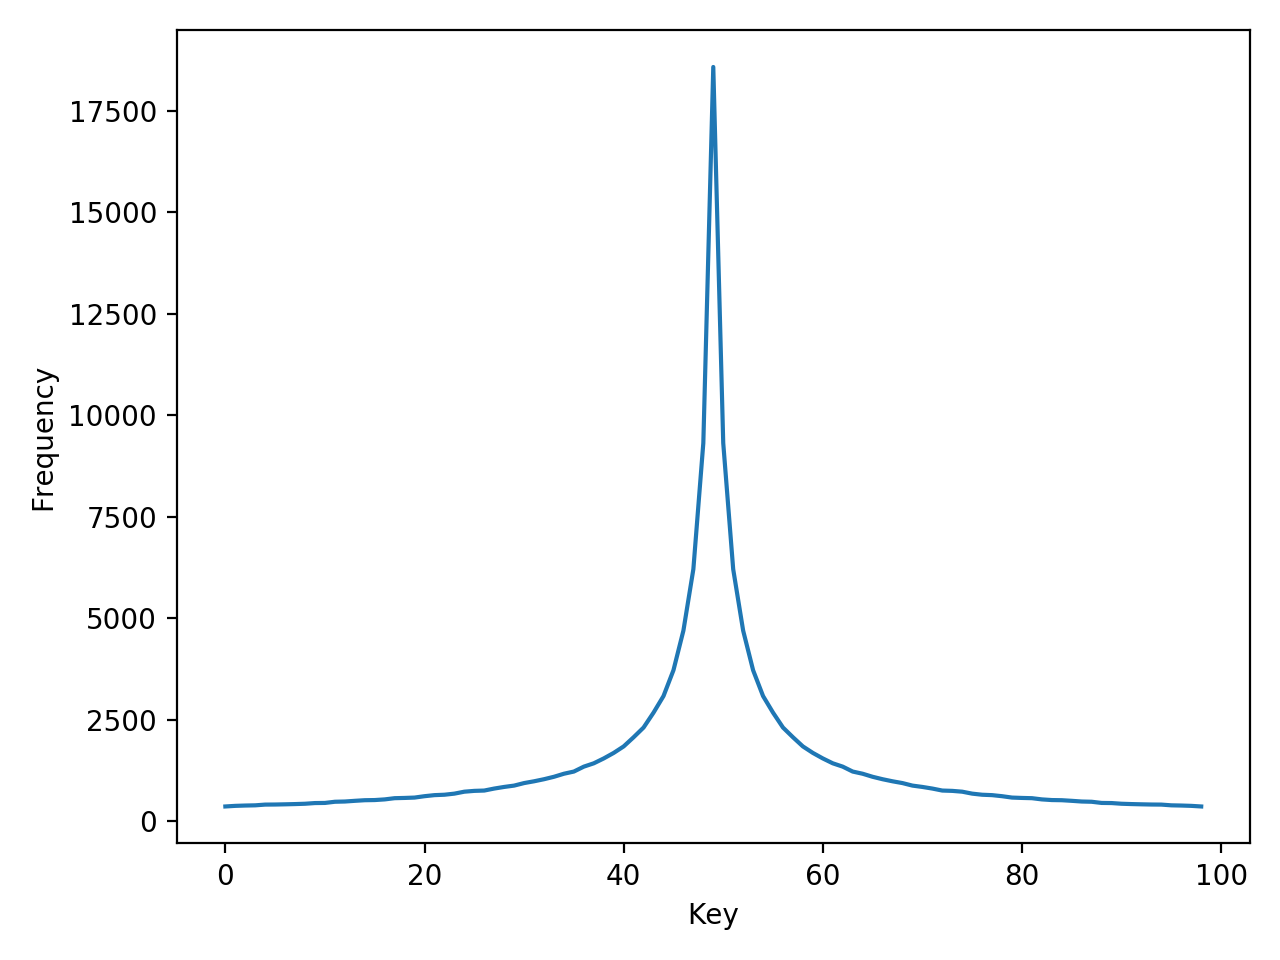
\includegraphics[width=0.49\textwidth,height=\textheight,keepaspectratio]{img/skew-alpha1smooth.png}
  \caption{ The different distributions used for the experiments}
  \label{fig:skews}
\end{figure}

Note that the zipf skew used in the tests is a slightly modified type of skew, which we call \emph{smooth skew}. The smooth skew is the symmetrical version of a normal skew. The last plot in Figure \ref{fig:skews} shows the smooth skew with $\alpha=1$. This allows us to have distributions that wraps around, with high locality between the values at the beginning and end of the range of keys.

The four plots shown in Figure \ref{fig:skews} are the different skew distributions obtained using different $\alpha$ values. We have top-left with $\alpha = 1$, top-right with $\alpha = 0.5$, bottom-left with $\alpha = 0$ and bottom-right with $\alpha = 1$ and smooth setting. The first three are quite self-explanatory, with the curve getting flatter and flatter the more we get close to zero. With the smooth curve it is important to notice that we are cutting the original curve in half, therefore the distribution will look slightly different compared to a non-smooth one with the same $\alpha$.
\\\\
The particular setups that we will test are four types of client behaviors, that we call \textbf{\emph{local-skewed}}, \textbf{\emph{global-skewed}}, \textbf{\emph{constant}} and \textbf{\emph{variable}}. For each of these, we will run tests with read/write ratios of 50, 90, 95, 99 (where 99 means 99\% of operations are  reads). For the tests we will have three groups. We will not perform tests with more groups, for two reasons. First, we expect the behavior of the system with an increasing number of groups to be similar, just slower, and in these tests we are not particularly interested in the maximum performance of the system. Second, we have already tested the performance of the repartition with more groups in the previous chapter.
\\\\
The tests will be run on a local cluster of machines, but with with simulated latencies between the replicas. These latencies were measured during the testing of GeoPaxos \citep{geopaxos} while it was tested on Amazon EC2 servers, and it was seen that the results of the real geographically distributed machines on EC2 nodes and the results with the simulated latencies were fairly similar. The simulated locations for the datacenters are in Tokyo(JP), California(CA) and Ireland(EU), with calculated latencies between the regions in Table~\ref{tab:latencies}. For the Paxos entities, the datacenters in each region contain 3 acceptors and one replica co-located with one of the acceptors. The latencies measured inside a datacenter were negligible, in the order of 1ms.


\begin{table}[!htb]
  \centering
  \begin{tabular}{l l l l}
    \hline
    & \textbf{EU} & \textbf{CA} & \textbf{JP} \\
    \hline
    \textbf{EU} & 1 & 145 & 215 \\
    \textbf{CA} & 145 & 1 & 145 \\
    \textbf{JP} & 215 & 145 & 1 \\
    \hline
  \end{tabular}
  \caption{The latencies, in milliseconds, used in our local cluster of machines used to simulate geographically distant datacenters, placed in Ireland(EU), California(CA) and Tokyo(JP)}\label{tab:latencies}
\end{table}

% [put image similar to GeoPaxos that shows replicas and latencies]

% \clearpage
\section{Local-skewed}\label{sec:local-skewed}
In a geographically distributed environment, one of the possible types of workloads that we expect to see is a workload that depends on the geographic location of the clients themselves. For example, we expect that the users from Europe will access objects related to news about Europe rather than America or Asia. Another similar example can be seen in social networks, where geographically close people have a higher chance of being connected.

Following this logic, the test we perform has three groups of clients in different regions that perform similar operations, but the distributions are shifted, so that they each focus on different key ranges. Figure ~\ref{fig:local-skewed-loads} shows a similar workload, with the $x$ axis representing the key of the object in the tree and the $y$ axis representing the frequency of operations on said object.

\begin{figure}[!htb]
  \centering
  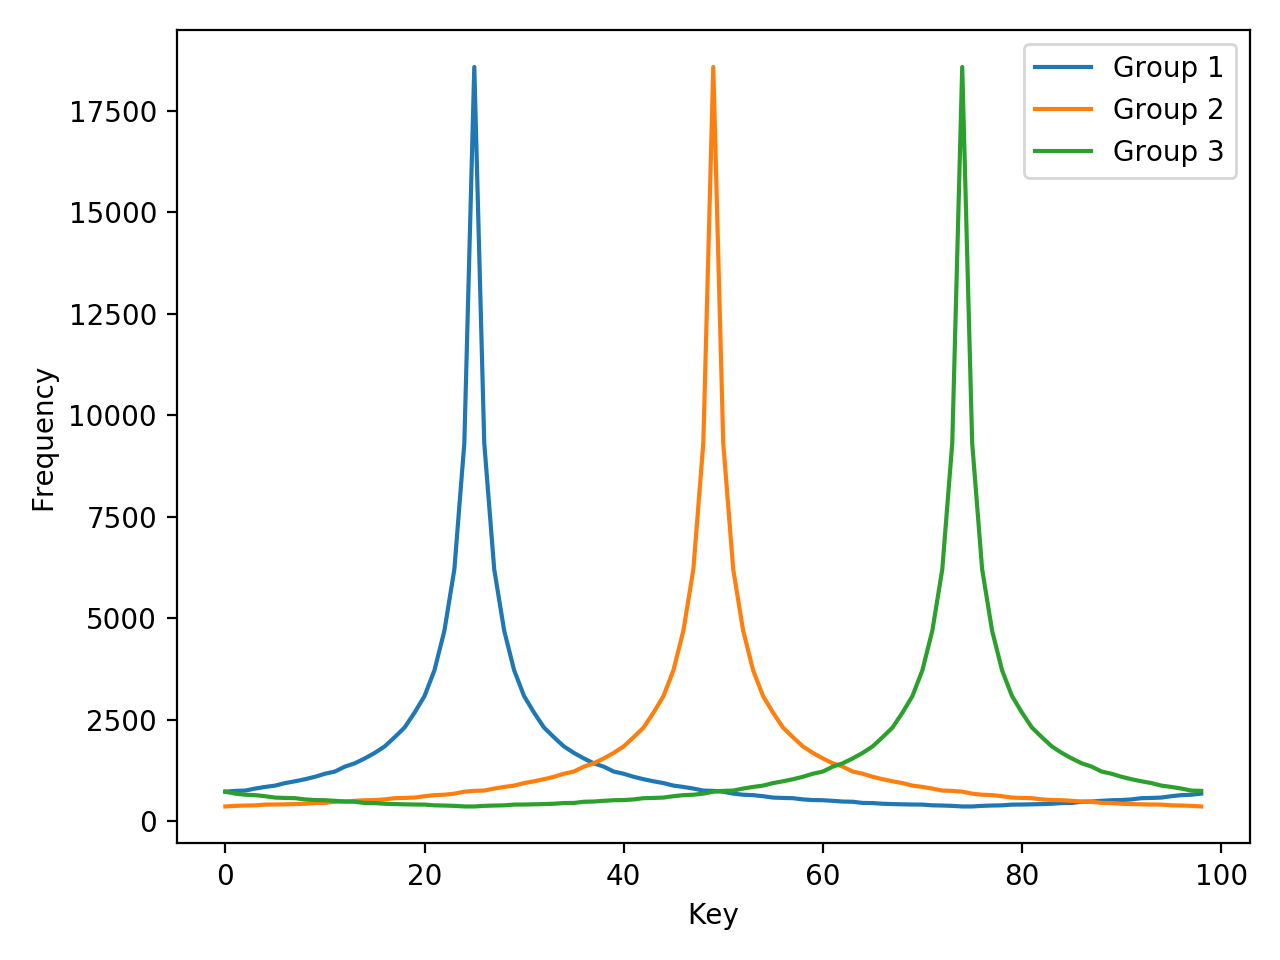
\includegraphics[width=\textwidth,height=\textheight,keepaspectratio]{img/clients_loads.png}
  \caption{ Distribution of client operations for the local-skewed tests }
  \label{fig:local-skewed-loads}
\end{figure}

Because this situation is the ideal case for GeoPaxos, we expect the performance to grow quite steadily after a few repartitions. This is because the shifted loads allow to assign the different areas to the different groups quite easily, allowing us to perform all the single group operations with almost no latency involved in the communications.

% \begin{figure}[!htb]
%   \centering
%   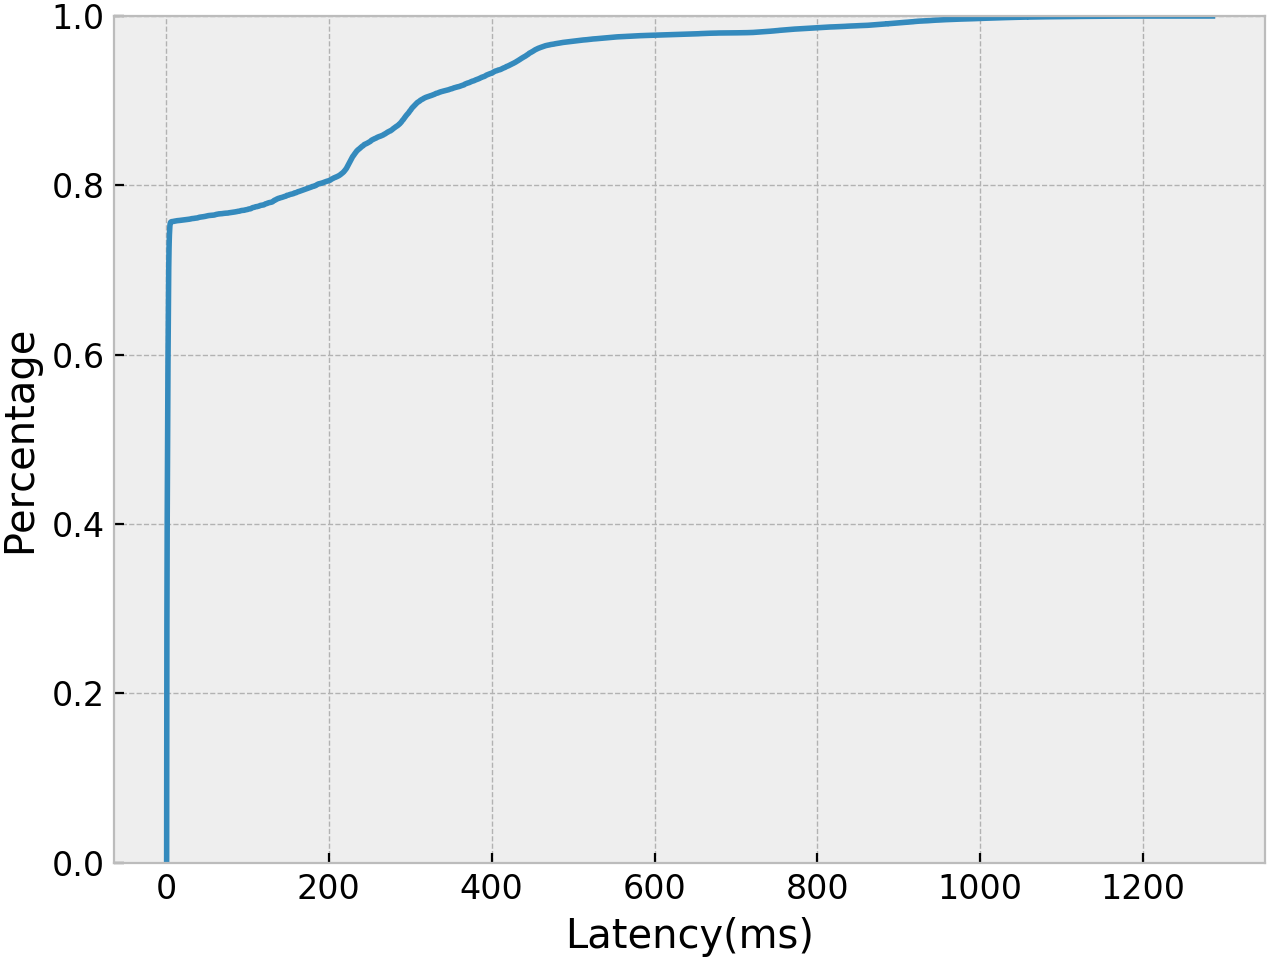
\includegraphics[width=0.49\textwidth,height=\textheight,keepaspectratio]{img/local50_lat.png}
%   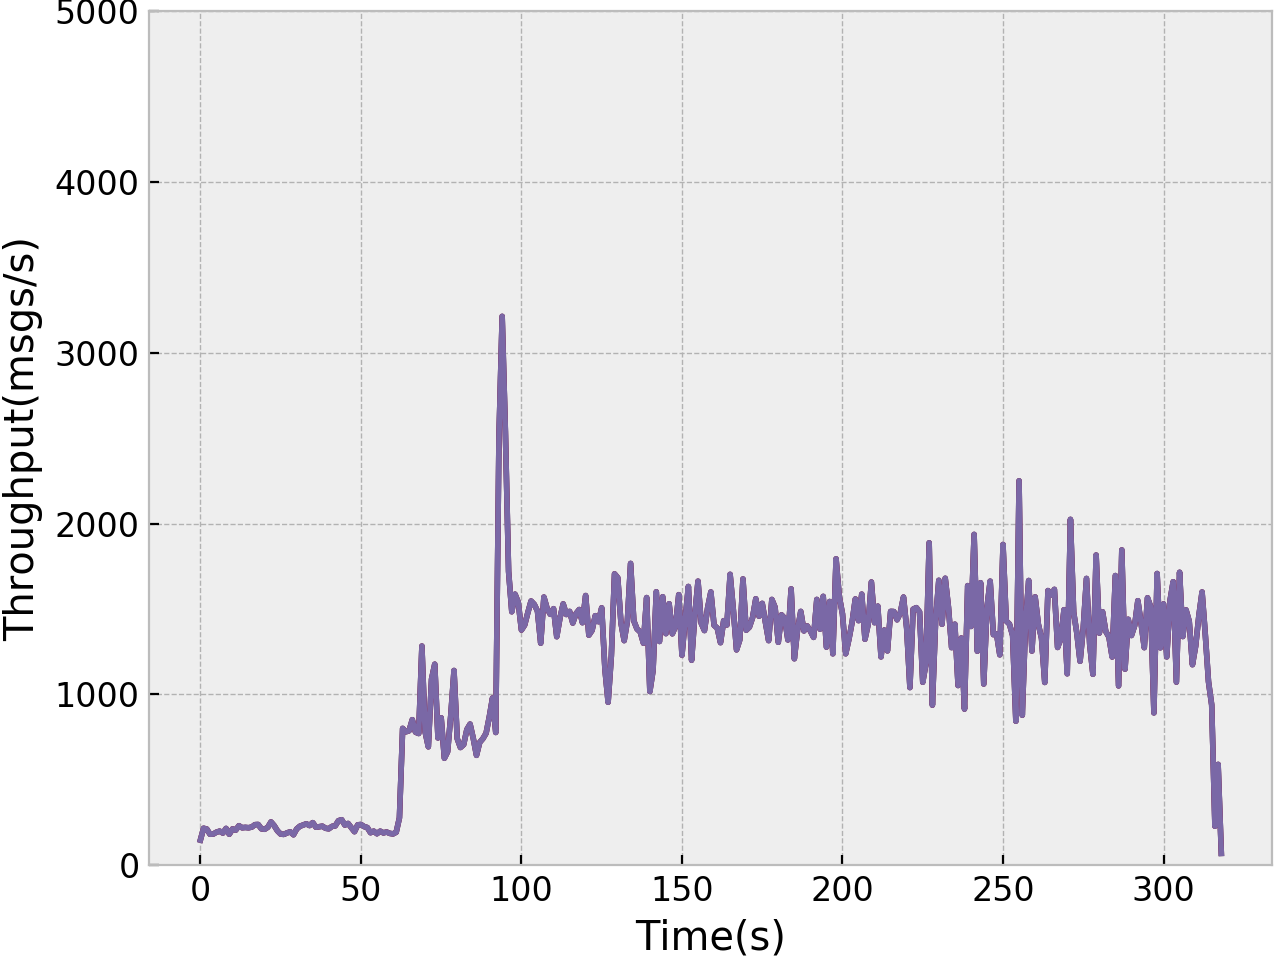
\includegraphics[width=0.49\textwidth,height=\textheight,keepaspectratio]{img/local50_tp.png}
%   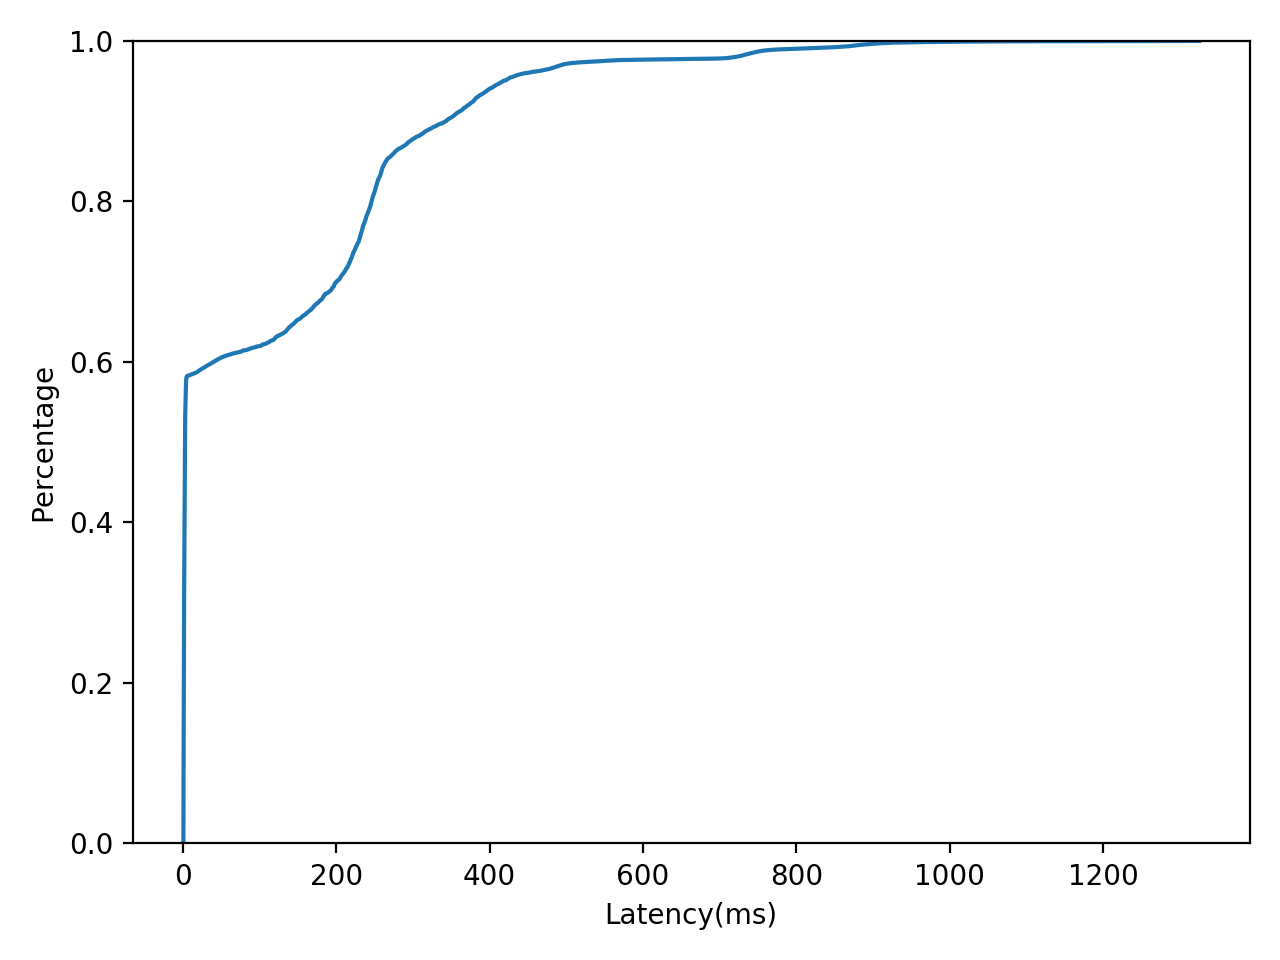
\includegraphics[width=0.49\textwidth,height=\textheight,keepaspectratio]{img/local10_lat.png}
%   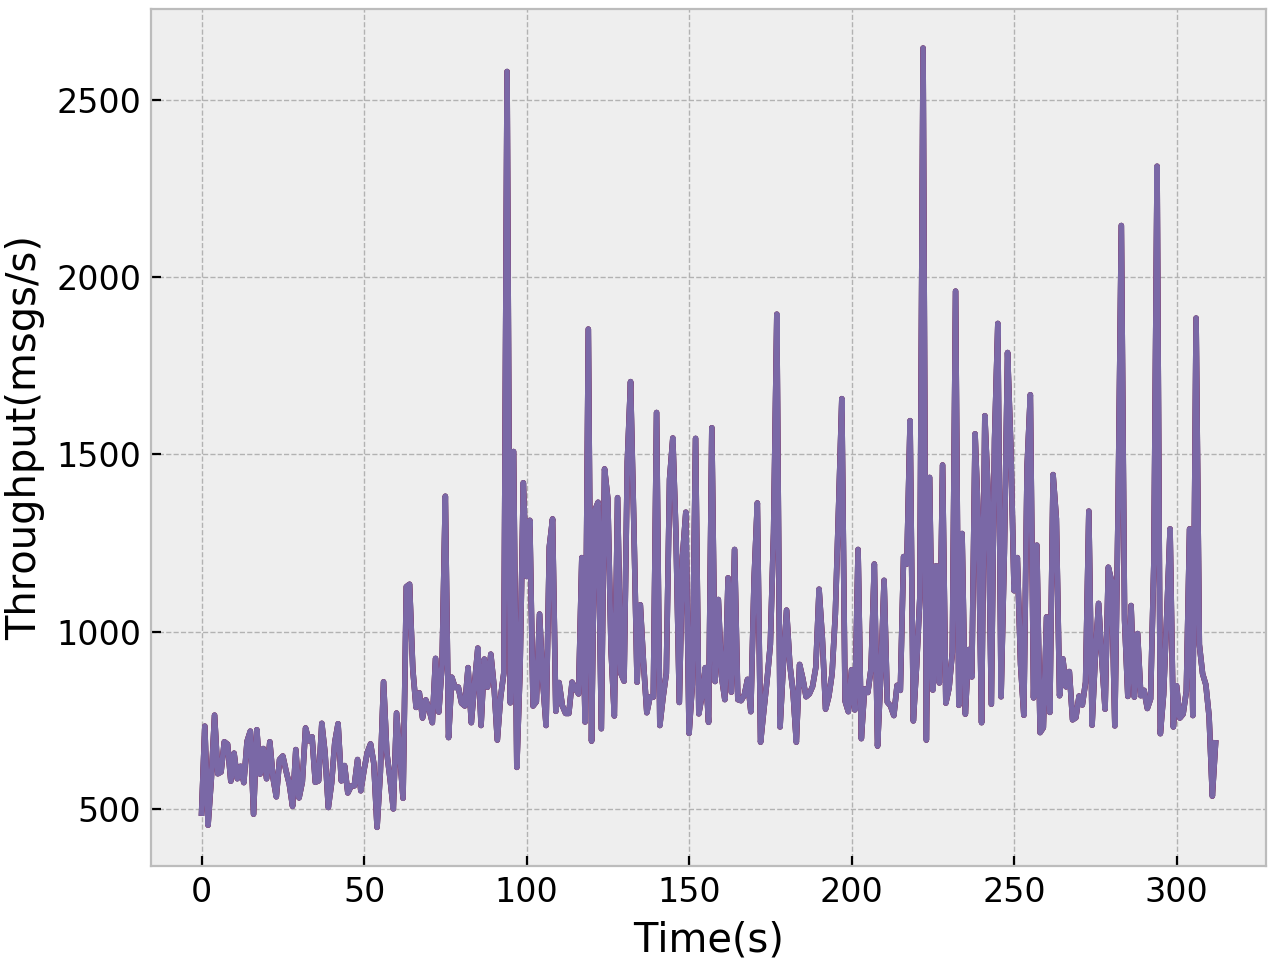
\includegraphics[width=0.49\textwidth,height=\textheight,keepaspectratio]{img/local10_tp.png}
%   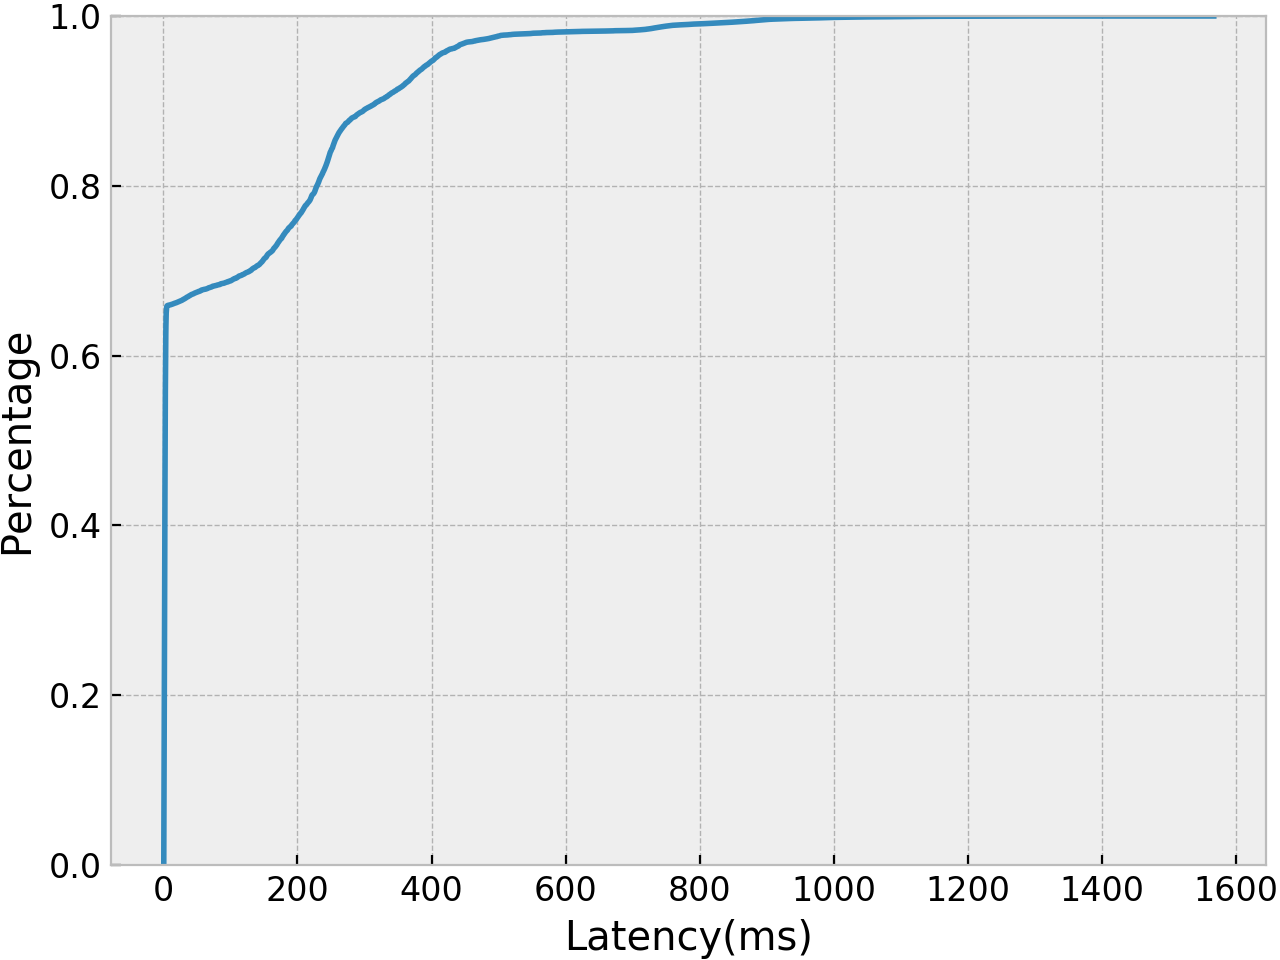
\includegraphics[width=0.49\textwidth,height=\textheight,keepaspectratio]{img/local5_lat.png}
%   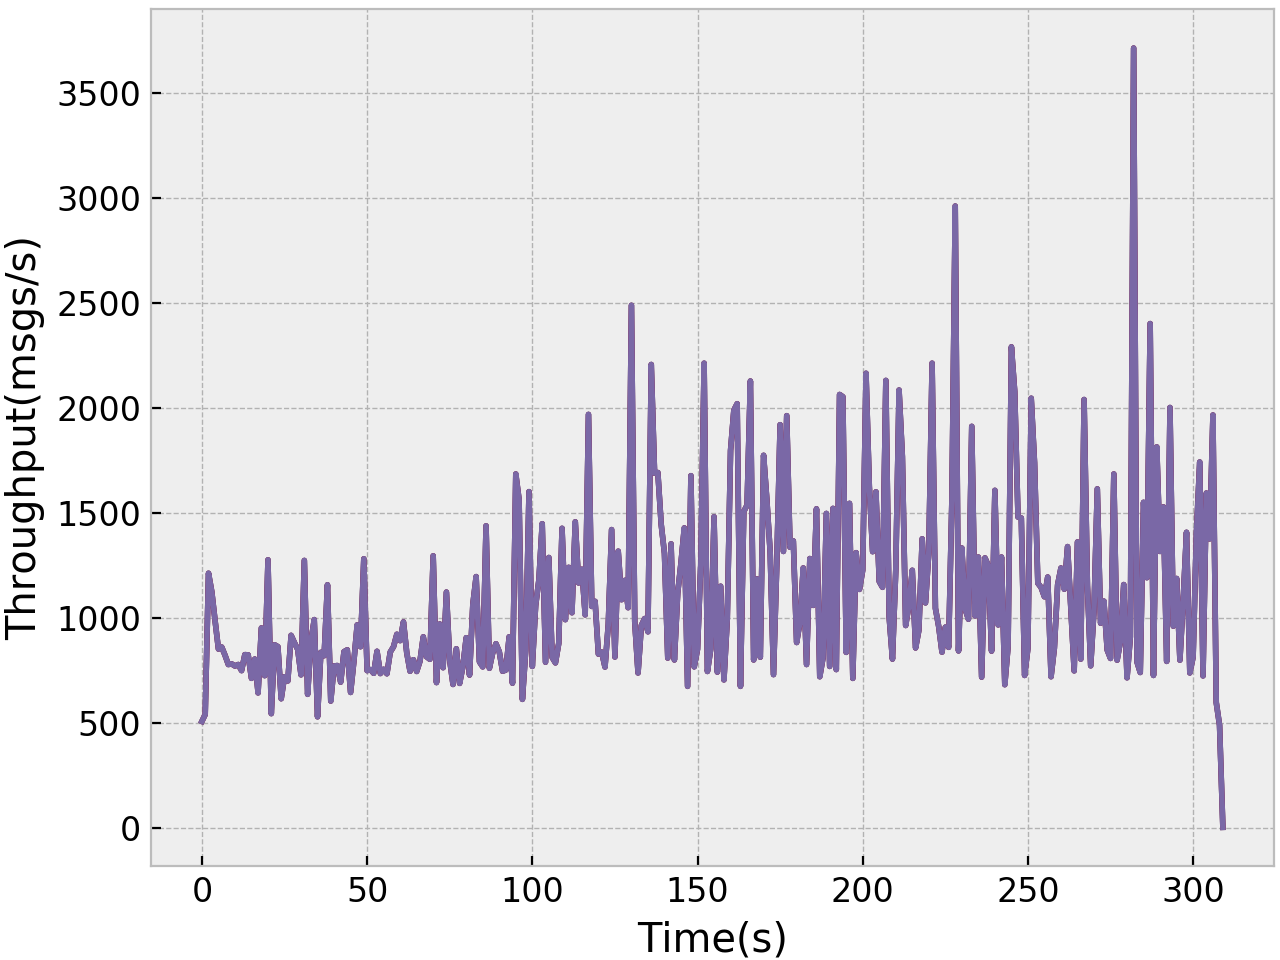
\includegraphics[width=0.49\textwidth,height=\textheight,keepaspectratio]{img/local5_tp.png}
%   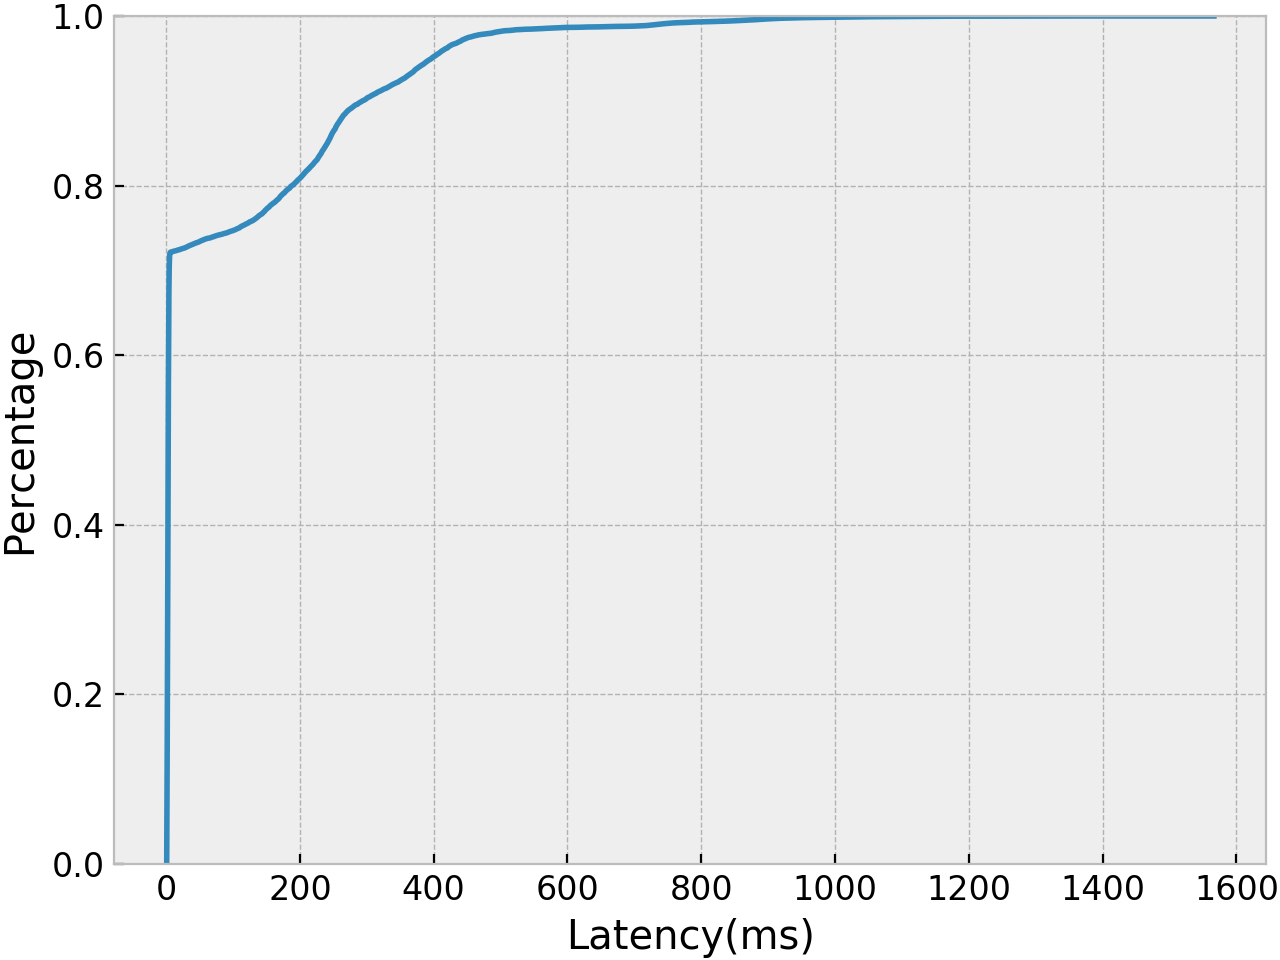
\includegraphics[width=0.49\textwidth,height=\textheight,keepaspectratio]{img/local1_lat.png}
%   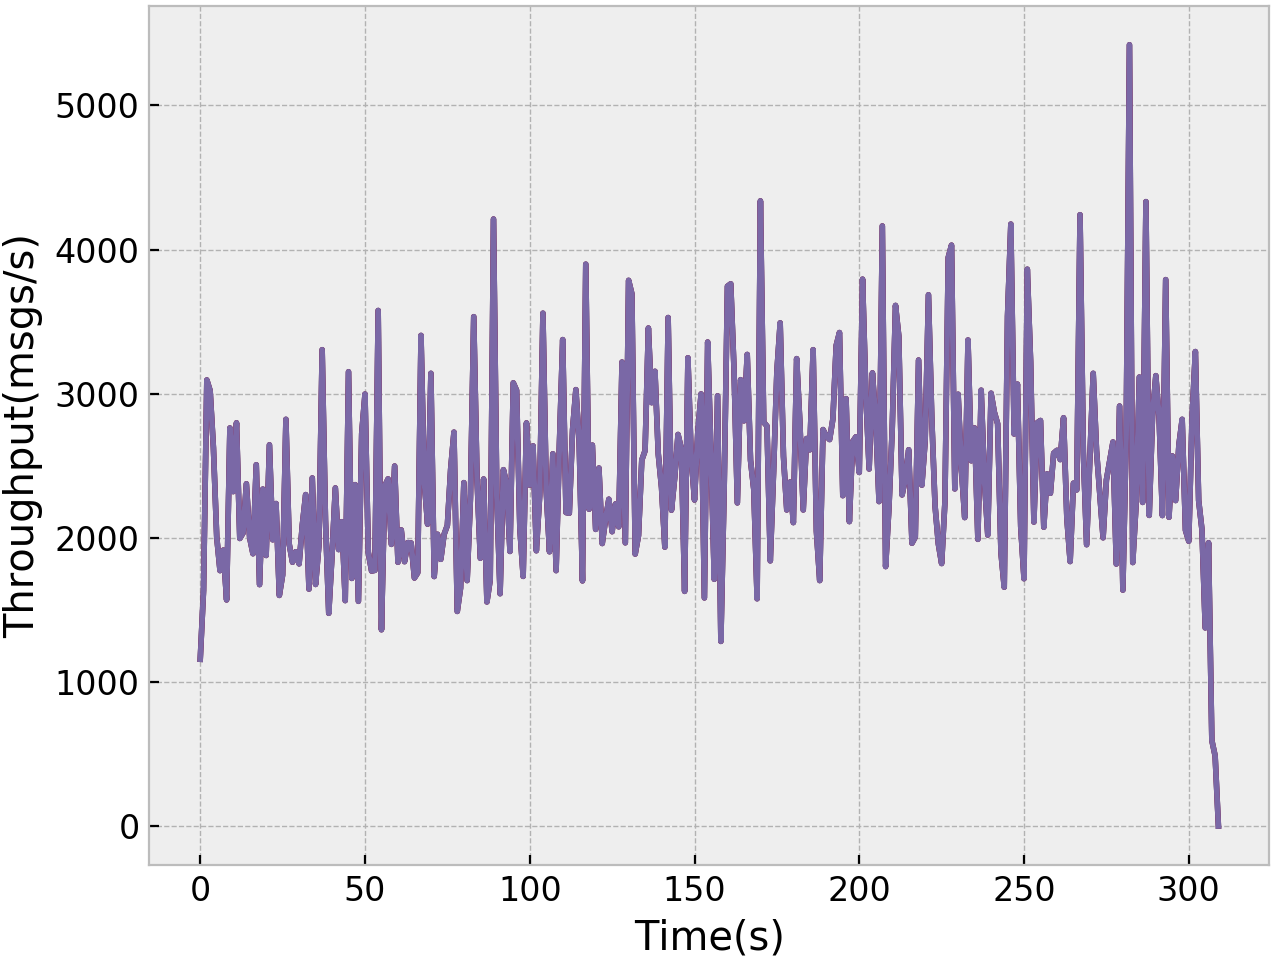
\includegraphics[width=0.49\textwidth,height=\textheight,keepaspectratio]{img/local1_tp.png}
%   \caption{ local tests with 50, 90, 95 and 99 percent reads }
%   \label{fig:local50-performance}
% \end{figure}

% \begin{figure}[!htb]
%   \centering
%   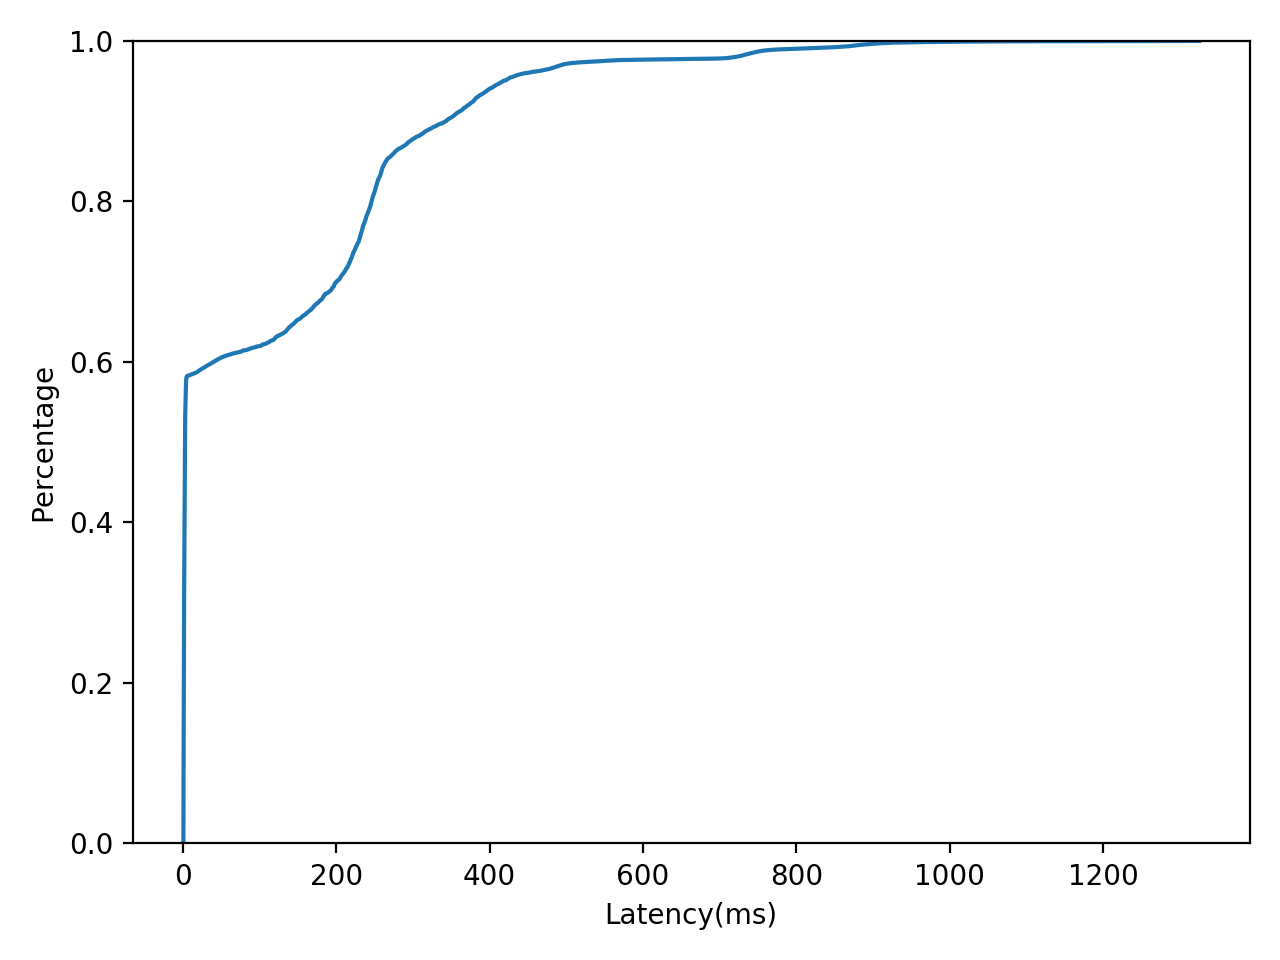
\includegraphics[width=0.49\textwidth,height=\textheight,keepaspectratio]{img/local10_lat.png}
%   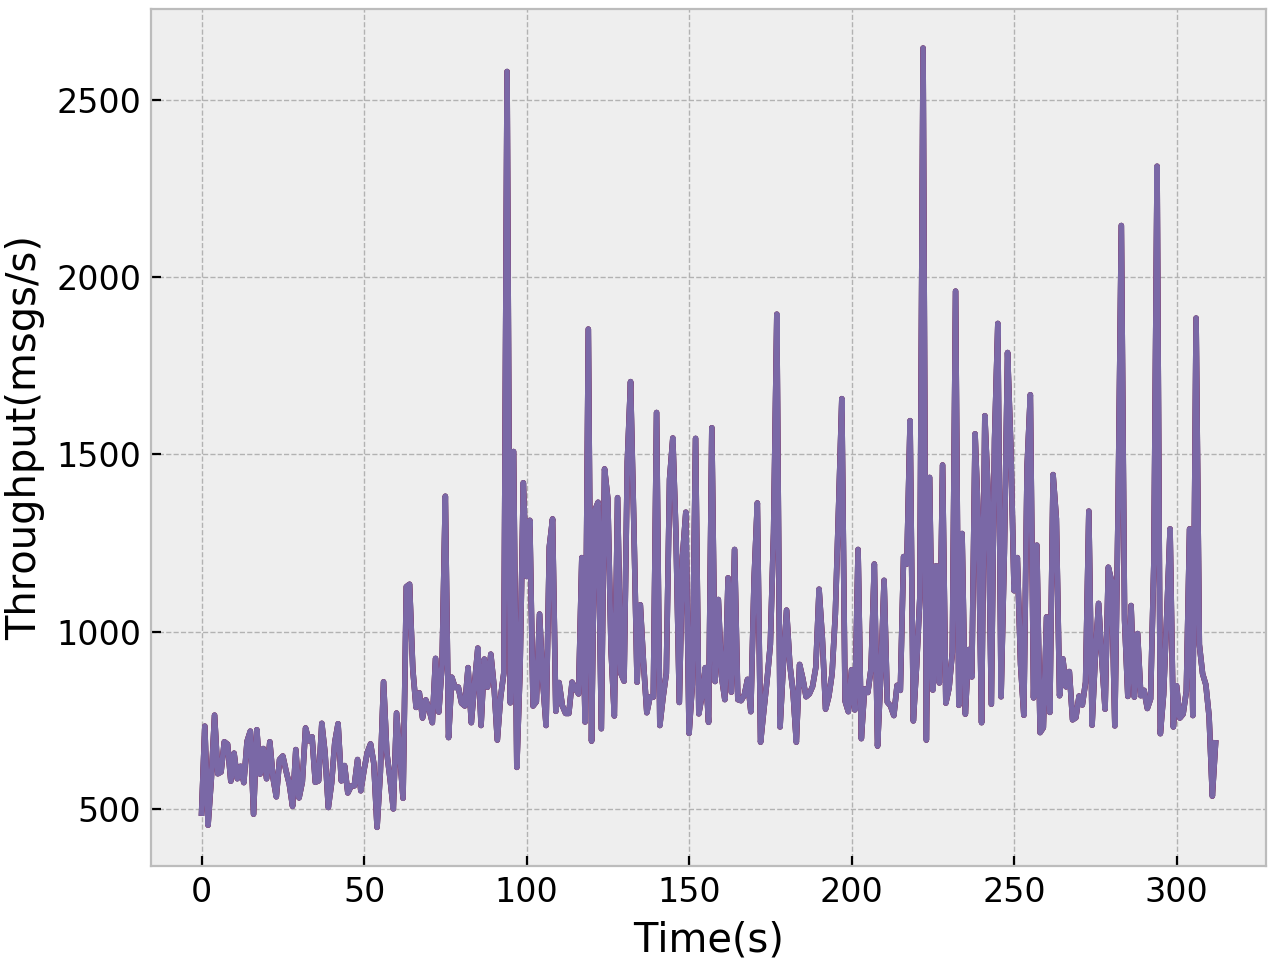
\includegraphics[width=0.49\textwidth,height=\textheight,keepaspectratio]{img/local10_tp.png}
%   \caption{ local test with 90\% reads }
%   \label{fig:local10-performance}
% \end{figure}

% \begin{figure}[!htb]
%   \centering
%   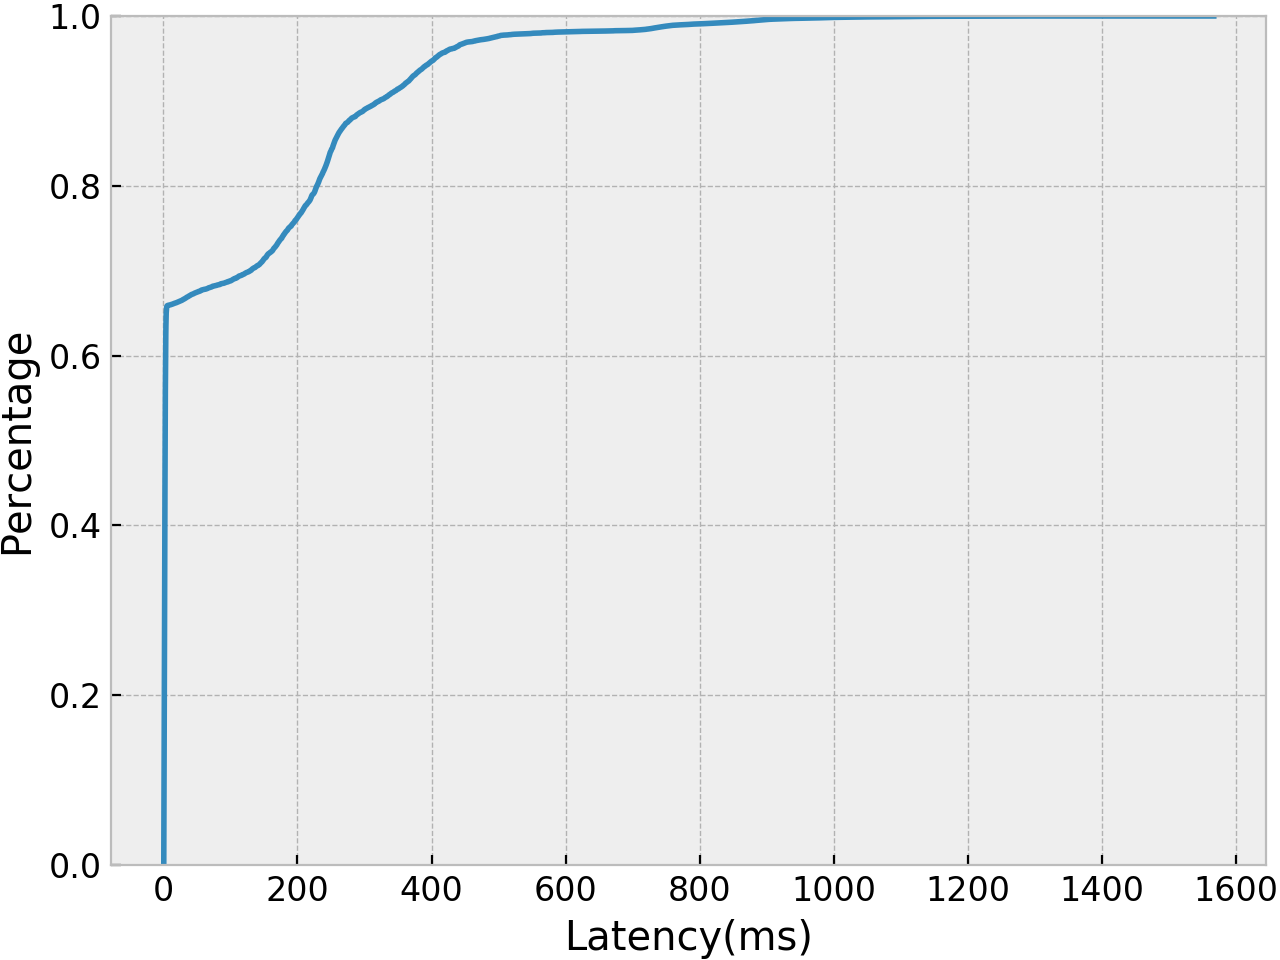
\includegraphics[width=0.49\textwidth,height=\textheight,keepaspectratio]{img/local5_lat.png}
%   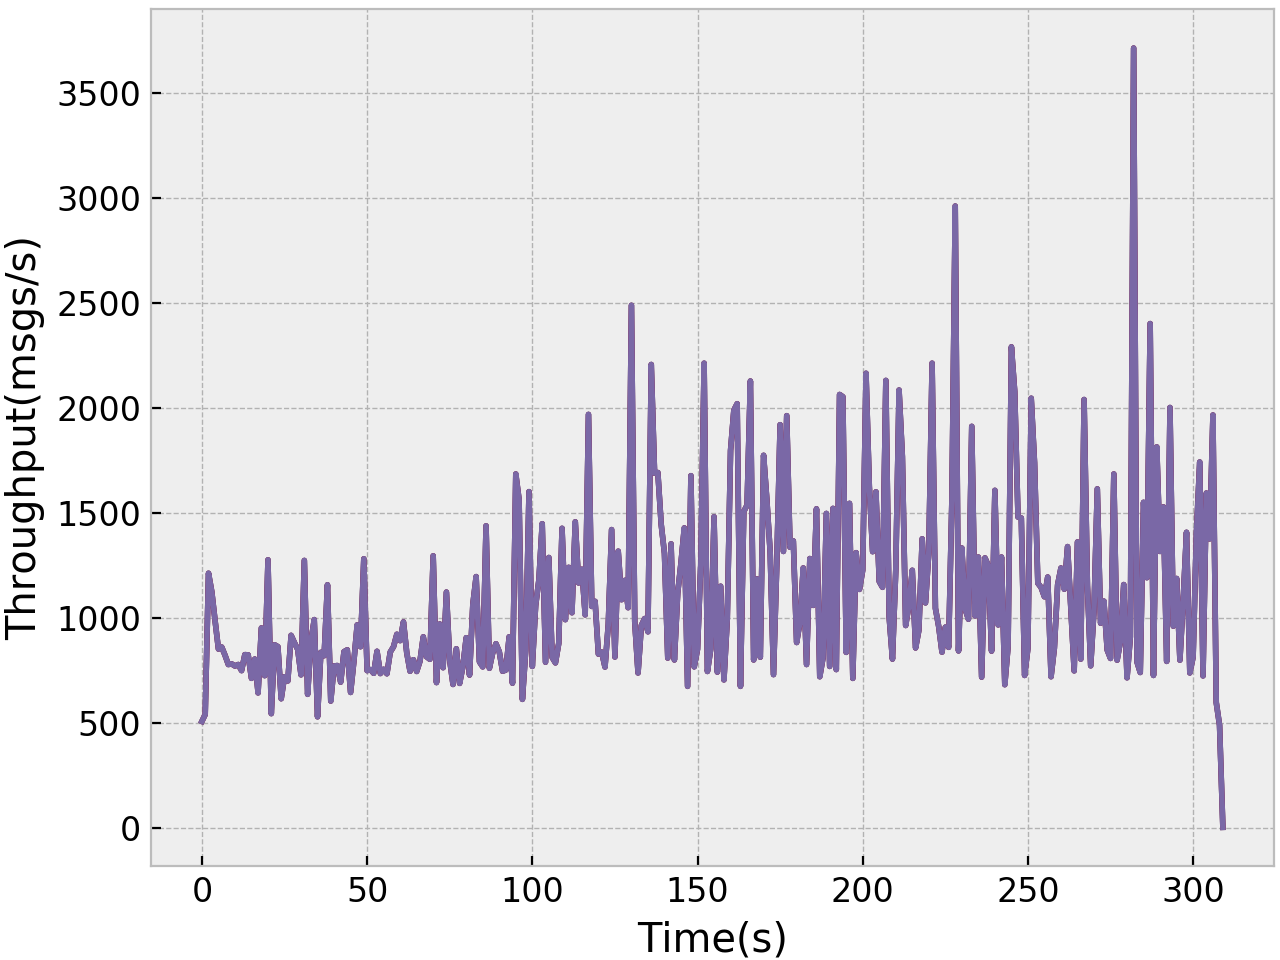
\includegraphics[width=0.49\textwidth,height=\textheight,keepaspectratio]{img/local5_tp.png}
%   \caption{ local test with 95\% reads }
%   \label{fig:local5-performance}
% \end{figure}

% \begin{figure}[!htb]
%   \centering
%   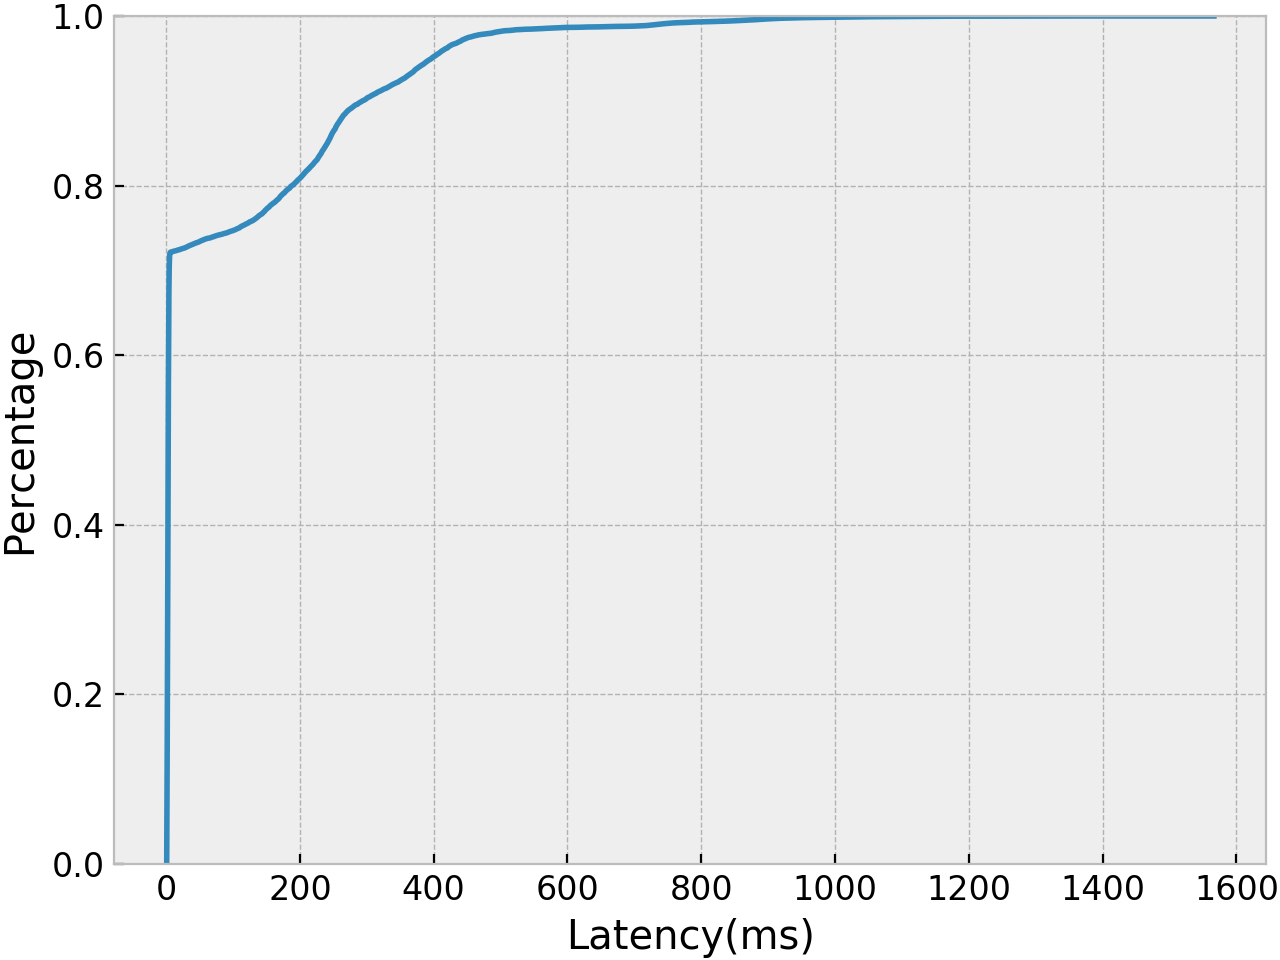
\includegraphics[width=0.49\textwidth,height=\textheight,keepaspectratio]{img/local1_lat.png}
%   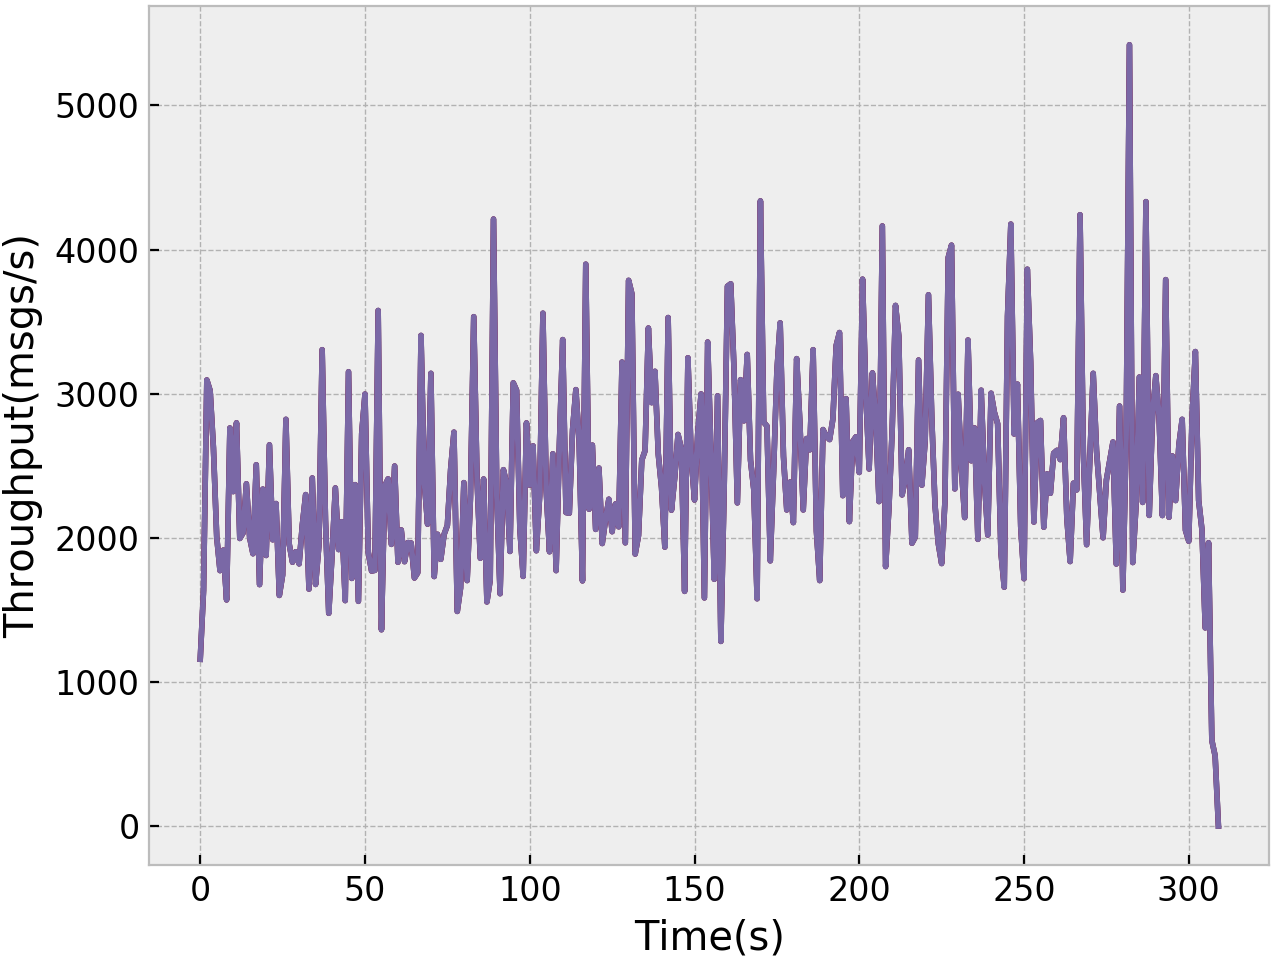
\includegraphics[width=0.49\textwidth,height=\textheight,keepaspectratio]{img/local1_tp.png}
%   \caption{ local test with 99\% reads }
%   \label{fig:local1-performance}
% \end{figure}

The results shown in Figure \ref{fig:local50-performance} regarding the tests with 90, 95 and 99 percent reads are pretty much as expected. The average throughput is slightly higher whenever we increase the amount of reads, since reads don't always require all the partitions to synchronize, allowing to perform multiple reads in parallel. The latencies follow a similar pattern, where the more reads we have, the lower the latencies are on average.

The unexpected results are with the test with 50\% reads, which surprisingly has both high throughput and many messages with low latency. Upon further inspection, we noticed that this was due to the repartitions assigning nodes to different groups. For the nodes handling keys that are evenly shared between groups (for example, in Figure \ref{fig:local-skewed-loads}, we see this around keys 0, 38, 62 and 100) the repartitioning algorithm assigns those nodes to only one group, while in the tests with higher reads percentages these nodes are assigned to all the groups (1, 2, 3). From the point of view of the algorithm, this makes sense: since in the first test we have 50\% reads, it is better to assign the nodes to only one group, to favor the write operations. Instead, in the tests with many reads, having these nodes assigned to multiple groups increases the performance with reads.

While this explains the different repartitioning, though, it still doesn't explain why an experiment with more writes shows better performance. The reason for the improved performance is that a repartition may cause a change in the future operations received. If, for example, the repartition gives the responsibility of ordering an object to a replica that is much closer to the previous one, then the operations on this object will be faster, which may allow some clients to perform more operations in the same amount of time. If this object is the only one whose responsibility was changed during the last repartition, we will have that the workloads before and after the repartition will be similar, except for the moved object. This means that the repartition has effectively influenced the workload. What is, then, the issue? the issue is that the repartition was optimizing the partitioning for the workload \emph{before} the repartition, not \emph{after}. 

Let's go back to our experiment with 50\% reads that had good performance. What happened was that, simply because of coincidence, the repartition was also better for the clients workload \emph{after} the repartition, while the repartition performed in the other experiments mainly favoured the workload previous to the repartition.

This shows one of the shortcoming of the way we calculate the optimized partitions. When the repartition algorithm assigns an object to a set of groups, it does not know how much this could affect the performance, it only knows that it minimizes the latency given the past workload. It might happen that one client was slowed down by high latency of the operations on this object, or it might be that the new partitions of this object give us very few improvements because the clients accessing this object were already at their maximum throughput.

This is definitely a limitation of our approach, though finding a solution to this problem would greatly increase the complexity of the system.
\\\\
Table \ref{tab:local-latencies-table} shows the mean and various percentiles regarding the timing of operations. They show similar results to the plots discussed above; in general the times are lower with an increasing percentage of reads, and we have the unexpectedly good performance of the 50\% reads experiment thanks to the different partitioning.

\begin{table}[!htb]
  \centering
  \begin{tabular}{l l l l l l l l}
    \hline
    & \textbf{Mean} & \textbf{5\%} & \textbf{25\%} & \textbf{50\%} & \textbf{75\%} & \textbf{95\%}& \textbf{99\%} \\
    \hline
    \textbf{50\% reads} & 82.75 & 0.866 & 1.074 & 1.964 & 4.632 & 436.6 & 876.2 \\
    \textbf{90\% reads} & 116.0 & 0.910 & 1.519 & 2.803 & 229.4 & 417.7 & 792.1 \\
    \textbf{95\% reads} & 96.98 & 0.983 & 1.832 & 2.829 & 186.8 & 404.9 & 782.8 \\
    \textbf{99\% reads} & 79.97 & 1.049 & 2.121 & 3.065 & 109.2 & 396.7 &  733.6 \\
    \hline
  \end{tabular}
  \caption{Mean latency and percentiles regarding the local-skewed experiments}\label{tab:local-latencies-table}
\end{table}

\begin{figure}[H]
  \centering
  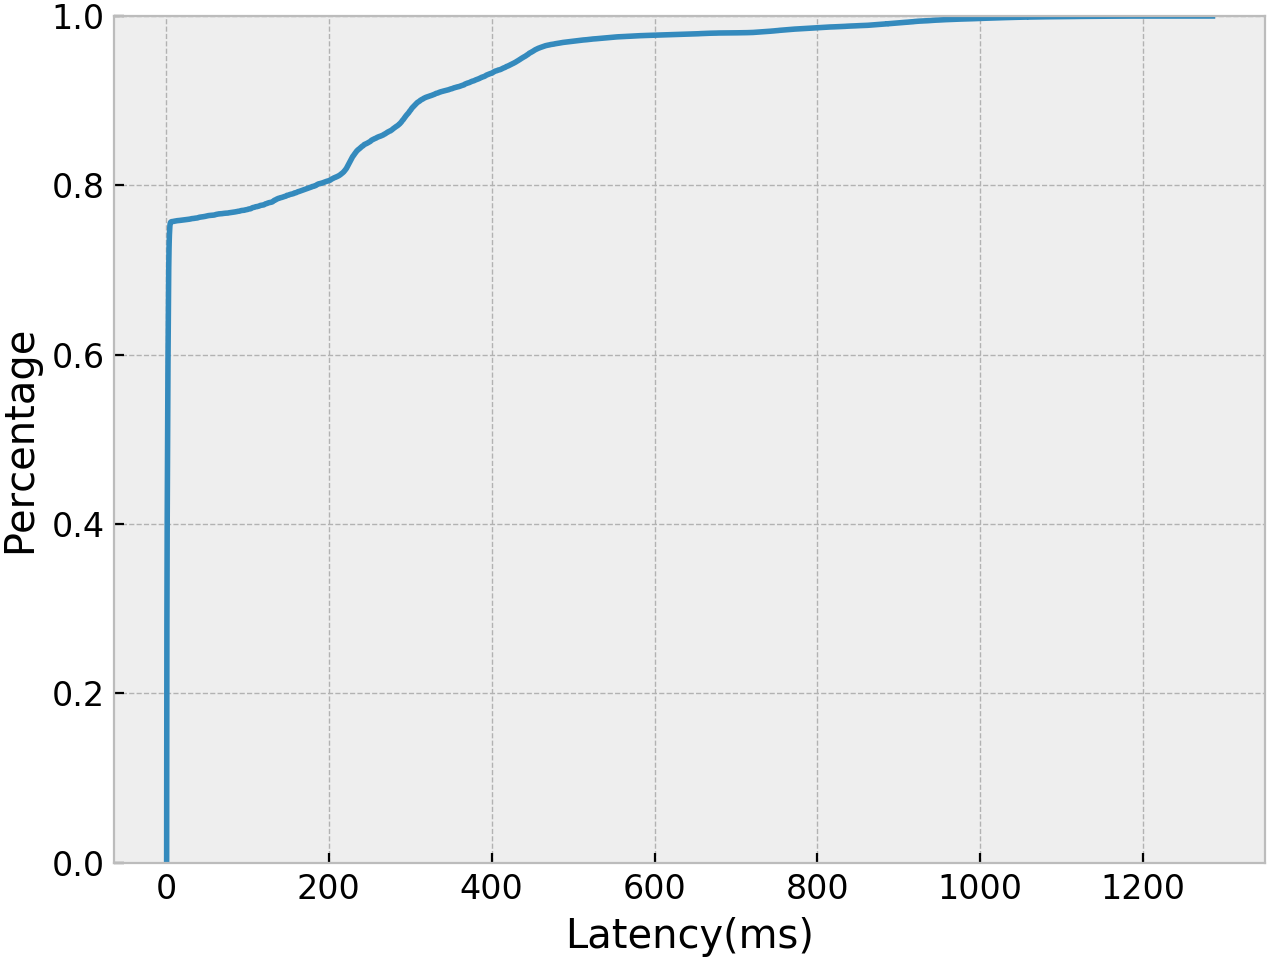
\includegraphics[width=0.49\textwidth,height=\textheight,keepaspectratio]{img/local50_lat.png}
  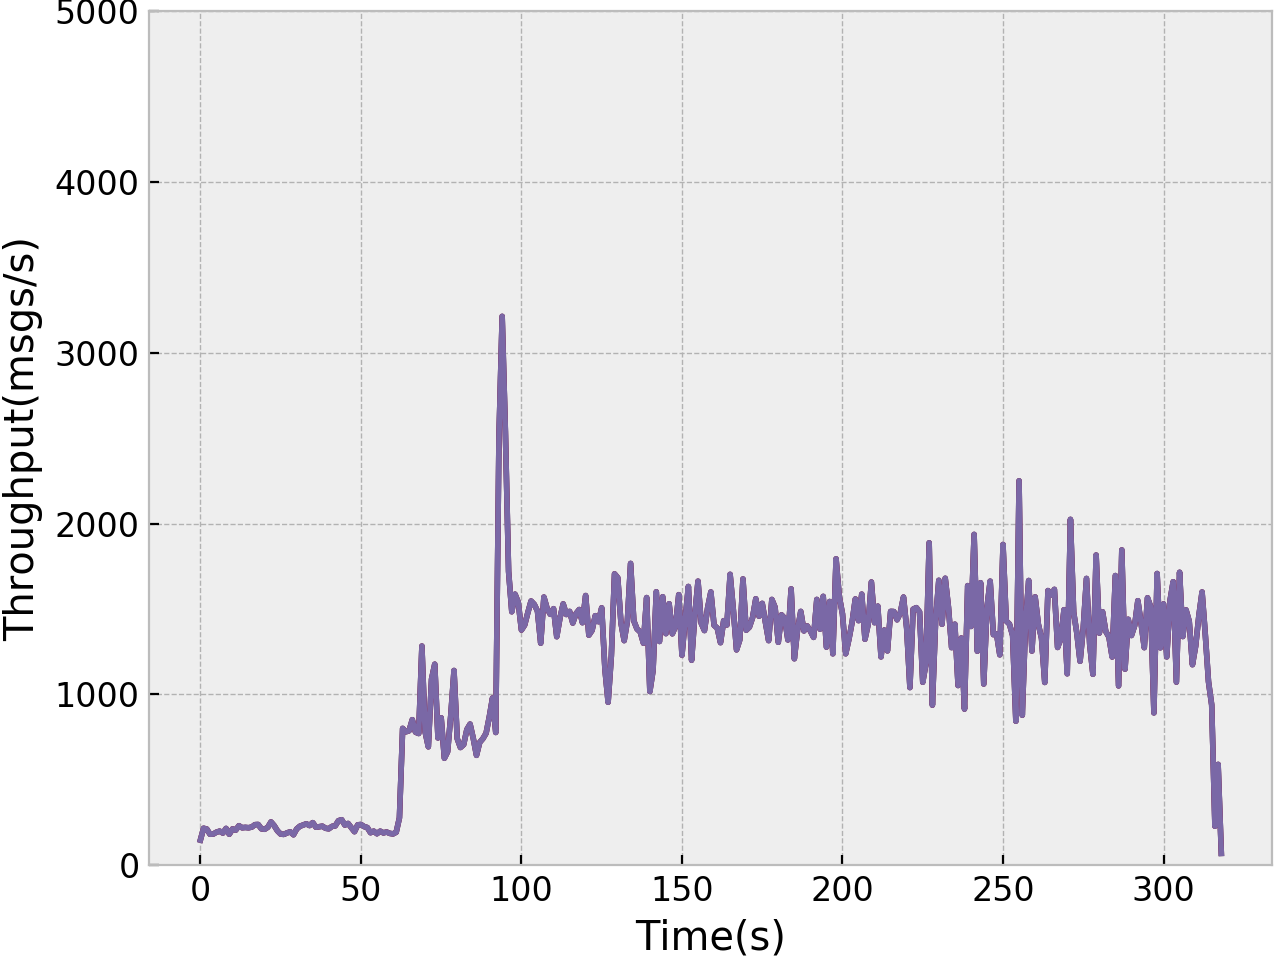
\includegraphics[width=0.49\textwidth,height=\textheight,keepaspectratio]{img/local50_tp.png}
  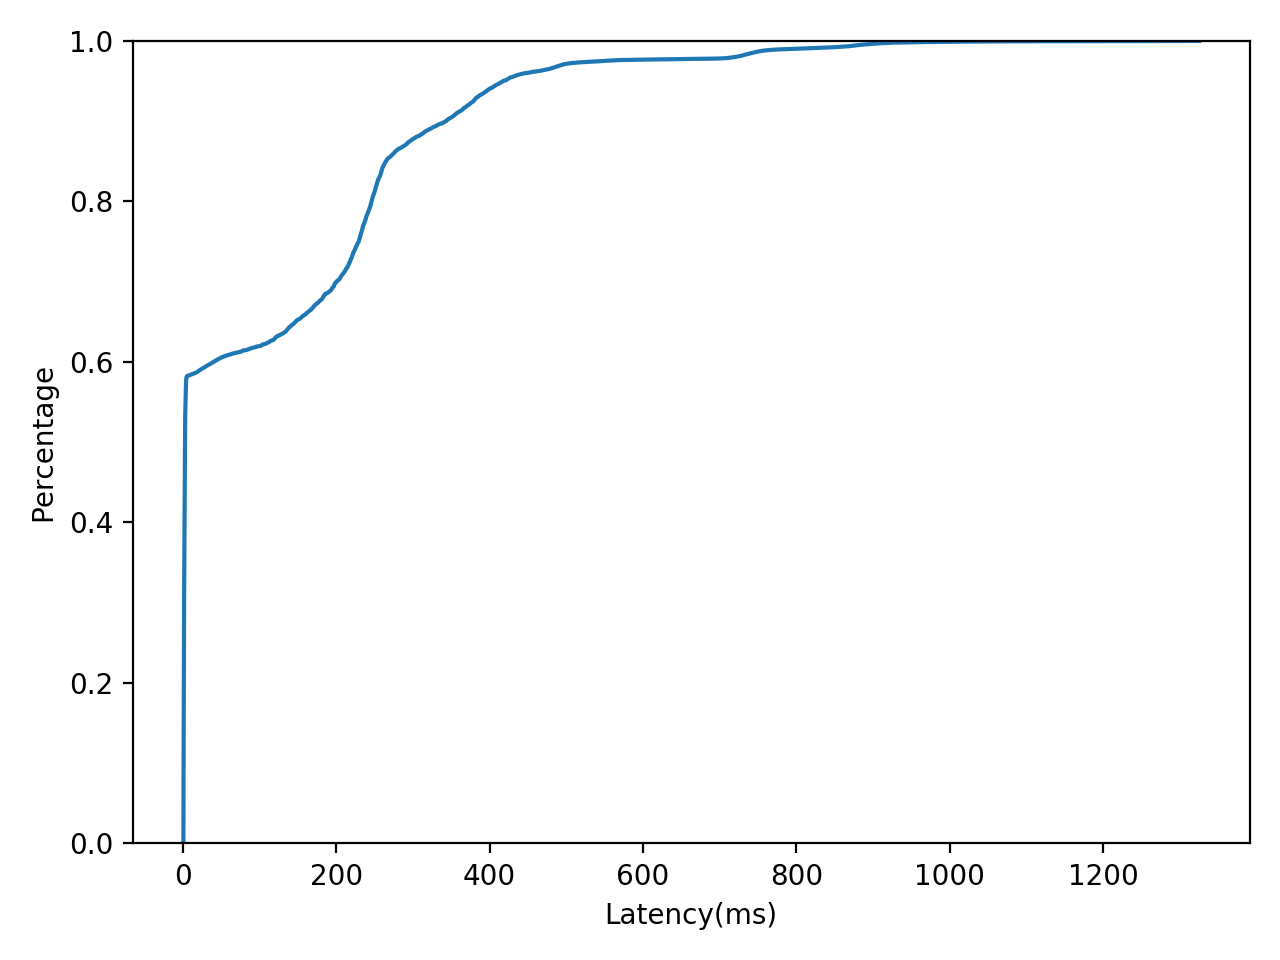
\includegraphics[width=0.49\textwidth,height=\textheight,keepaspectratio]{img/local10_lat.png}
  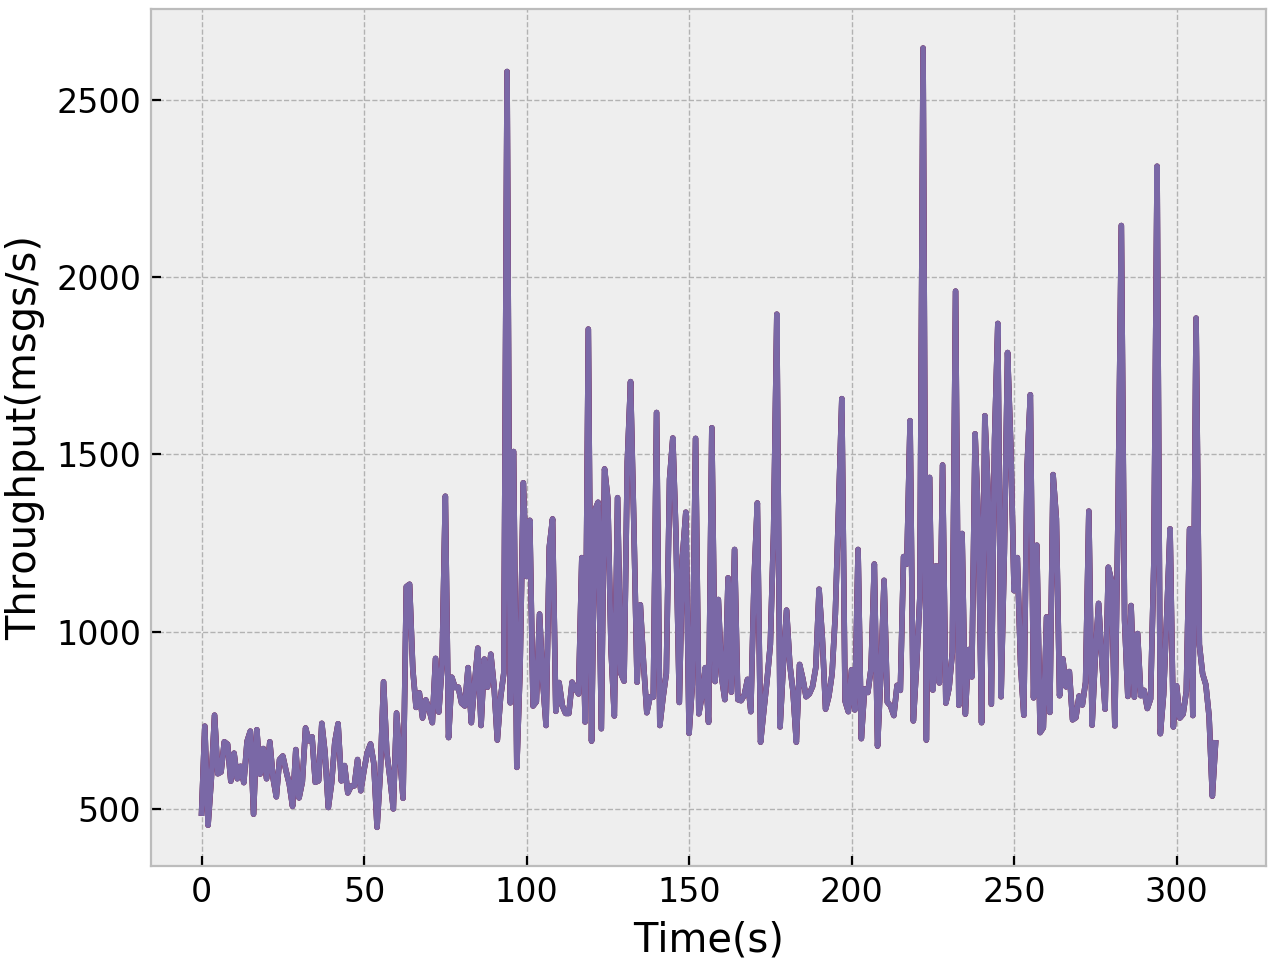
\includegraphics[width=0.49\textwidth,height=\textheight,keepaspectratio]{img/local10_tp.png}
  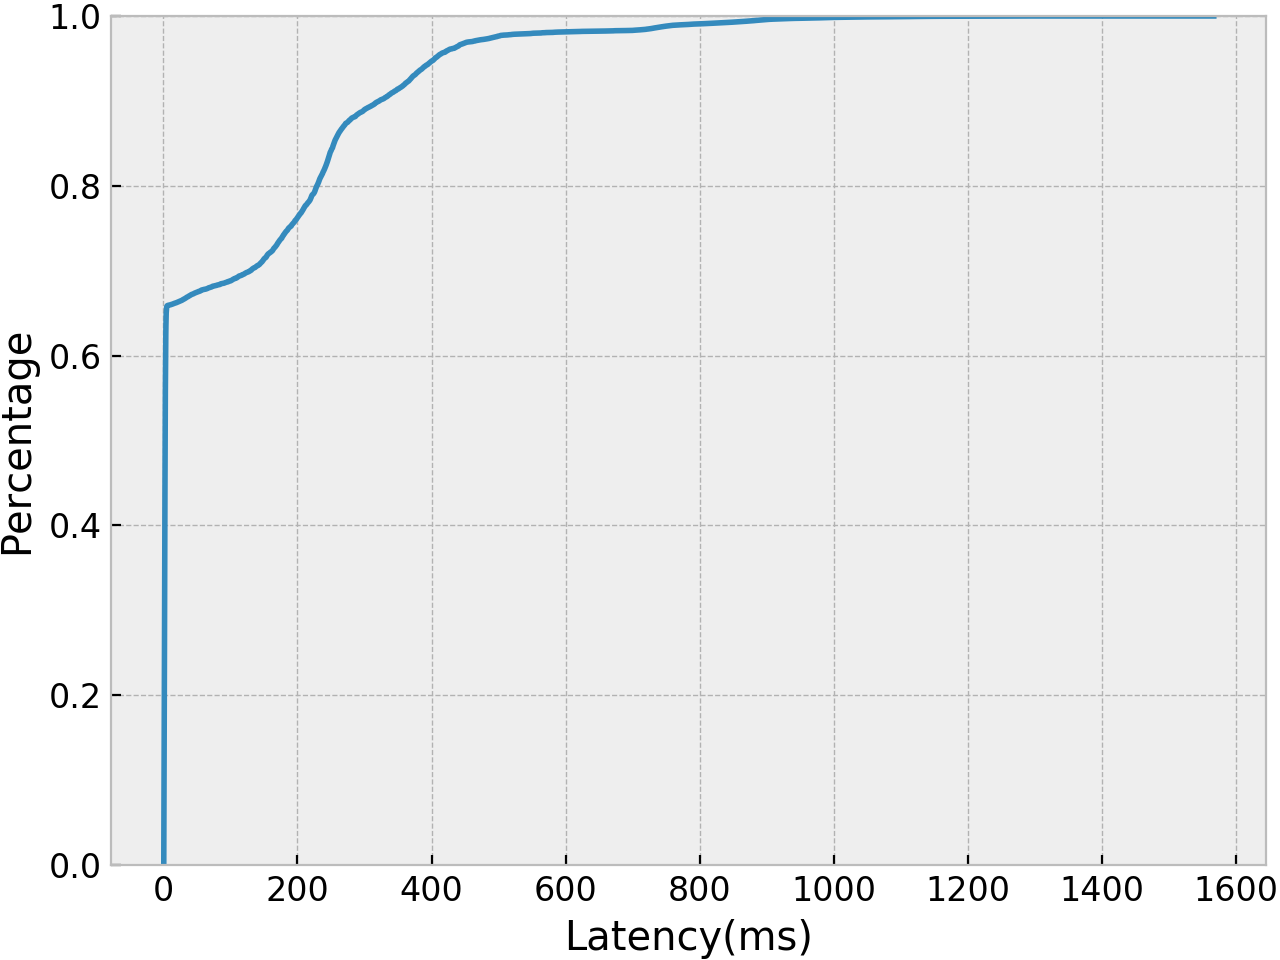
\includegraphics[width=0.49\textwidth,height=\textheight,keepaspectratio]{img/local5_lat.png}
  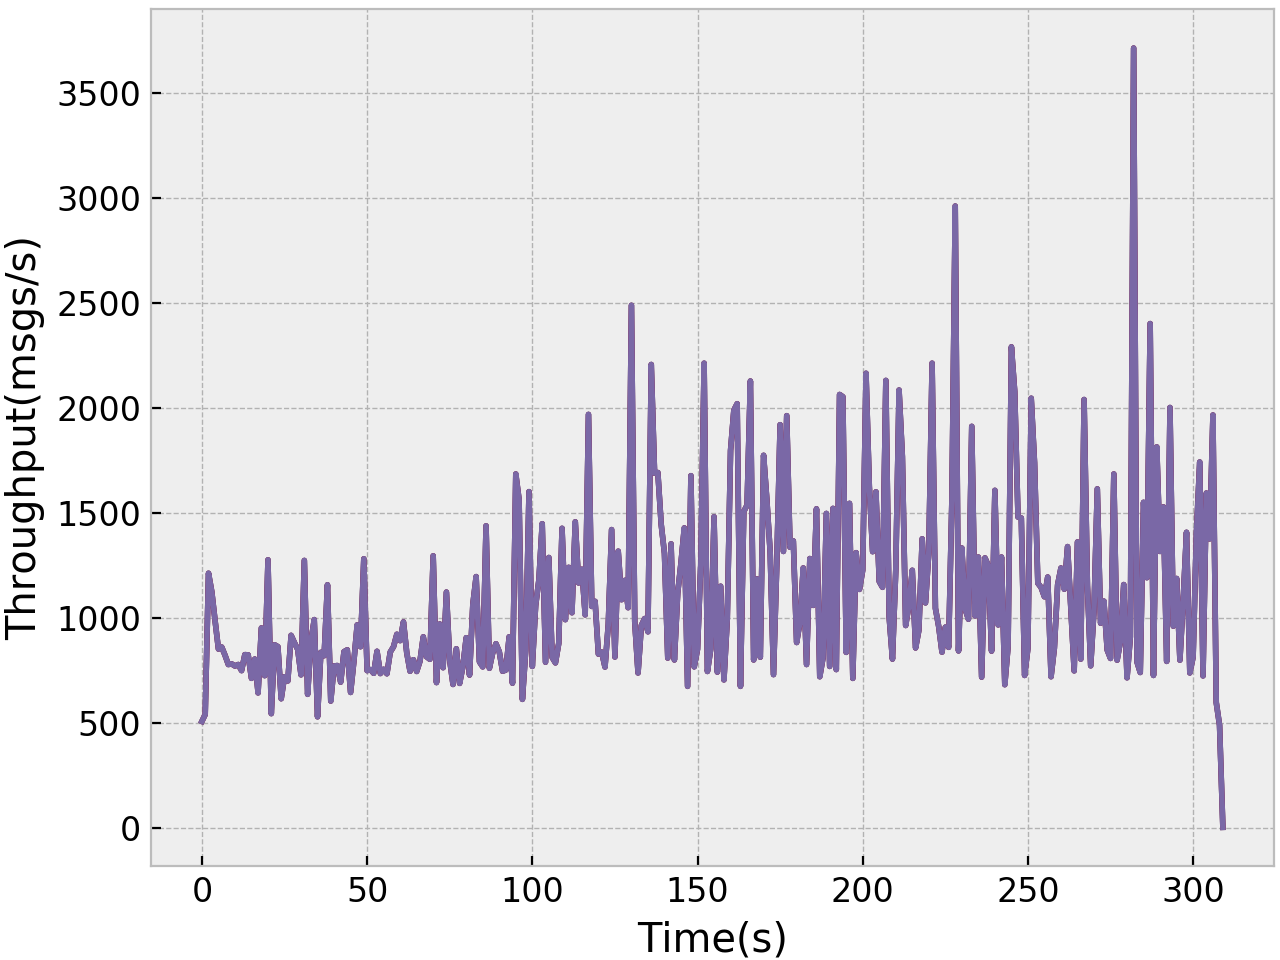
\includegraphics[width=0.49\textwidth,height=\textheight,keepaspectratio]{img/local5_tp.png}
  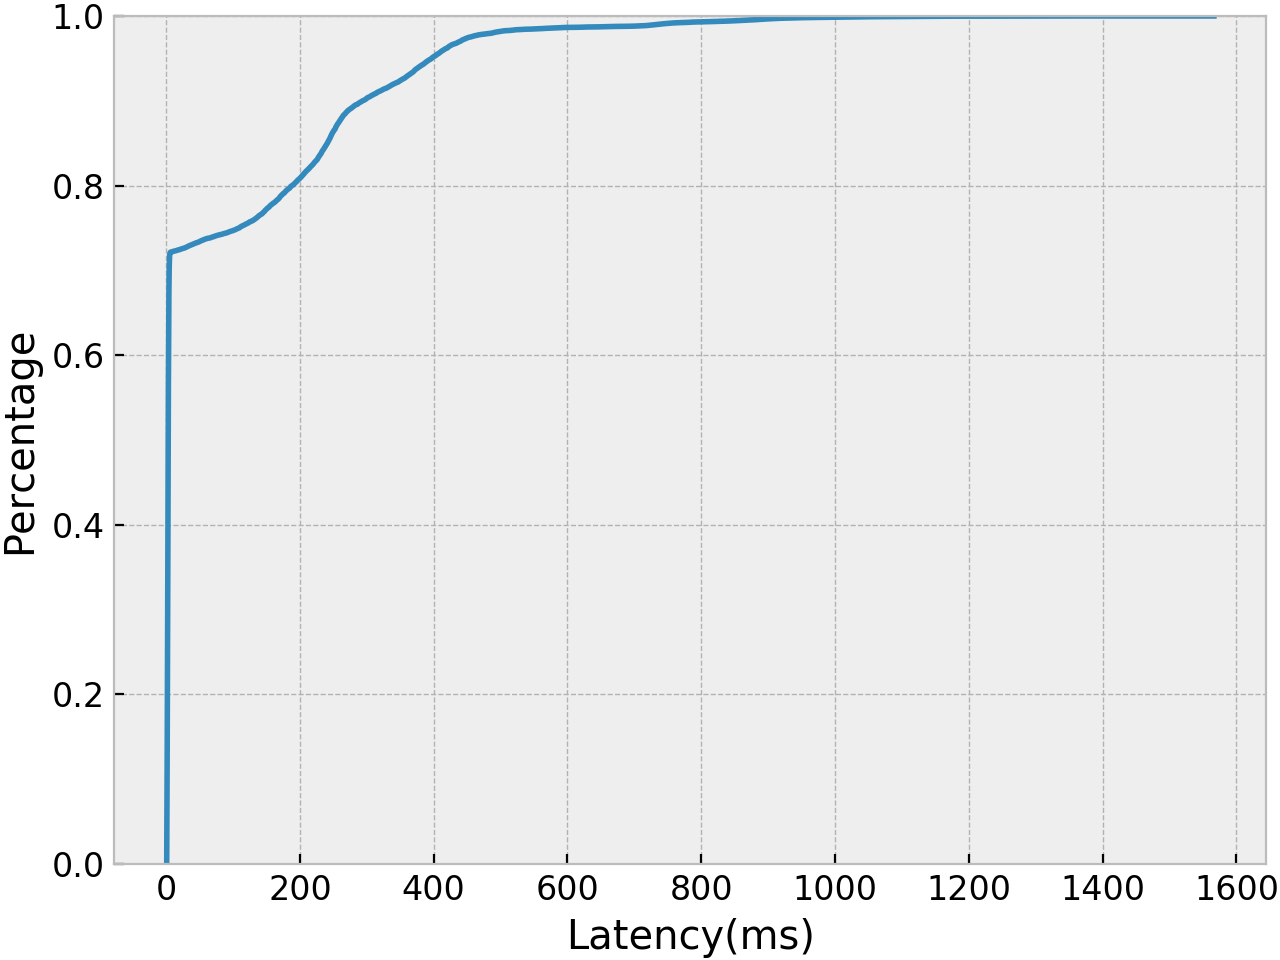
\includegraphics[width=0.49\textwidth,height=\textheight,keepaspectratio]{img/local1_lat.png}
  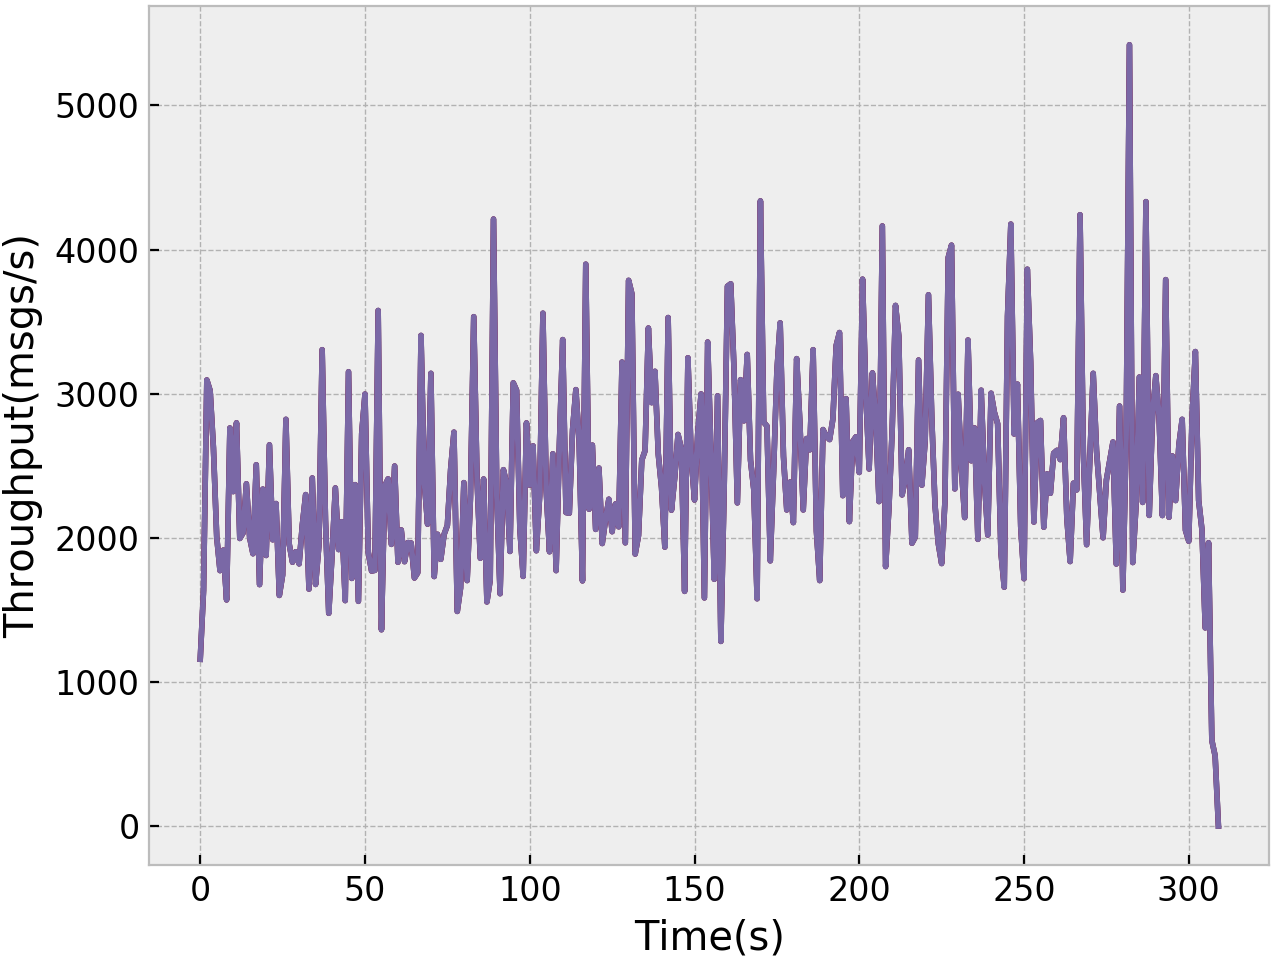
\includegraphics[width=0.49\textwidth,height=\textheight,keepaspectratio]{img/local1_tp.png}
  \caption{ CDF of latency on the left and throughput versus time on the right }
  \label{fig:local50-performance}
\end{figure}

\section{Global-skewed}\label{sec:global-skewed}
Another possible view on client behavior in geographically distributed environments is the opposite of the previous one. Instead of having ``local loads'' that depend on the geographic locations of the clients, we could instead have one global load that is shared among all the clients. Examples of objects that could lead to this behavior are viral news that could interest the whole world, or famous people that have fans from all across the globe.

For the test we have similar loads as before, but this time they are not shifted, which means that all clients access the same keys with the same distribution. This can be seen in Figure \ref{fig:global-skewed-loads}.

\begin{figure}[!htb]
  \centering
  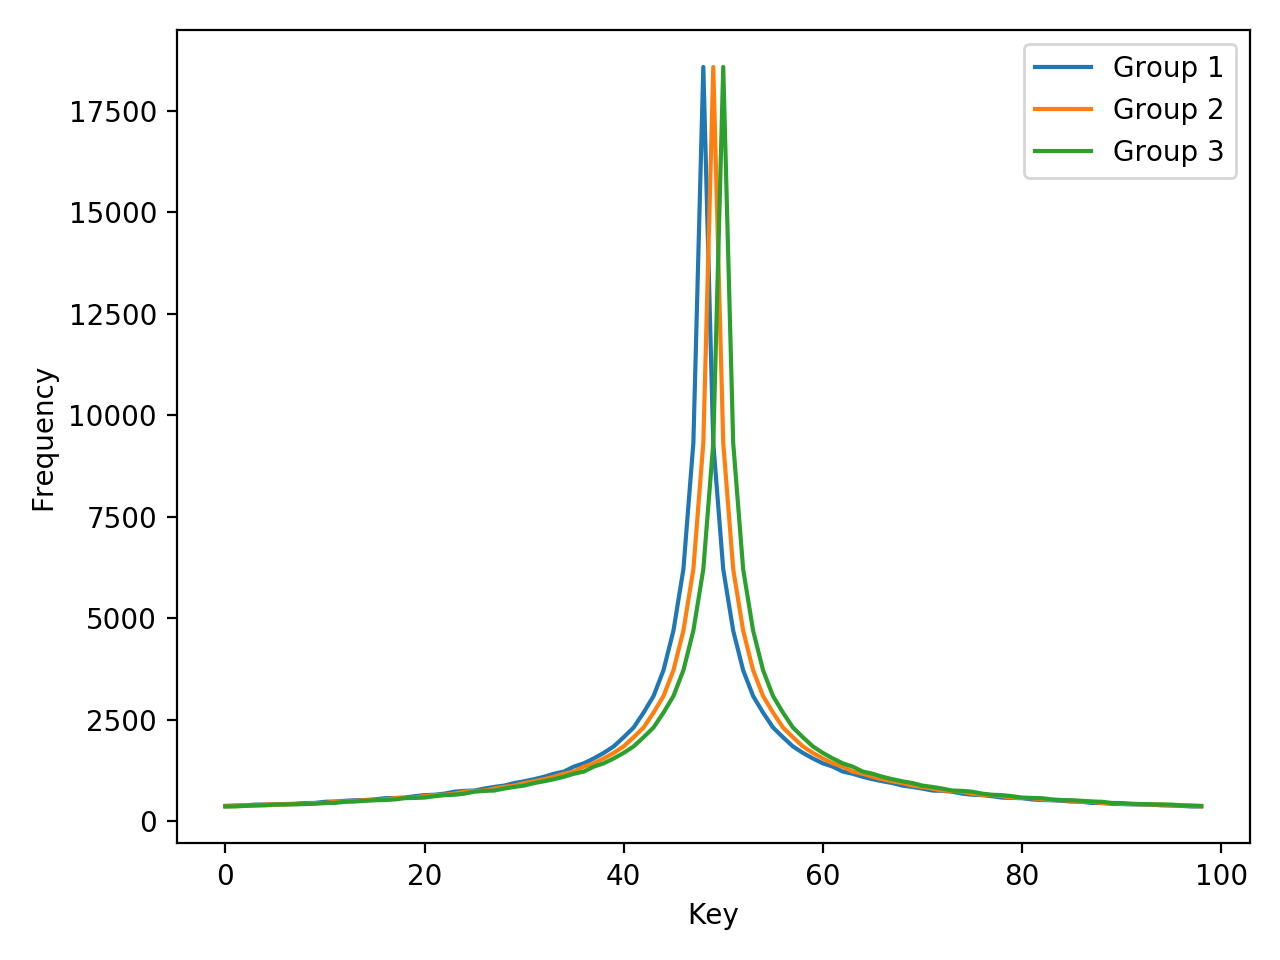
\includegraphics[width=\textwidth,height=\textheight,keepaspectratio]{img/clients_loads_global.png}
  \caption{ Distribution of client operations for the global-skewed tests }
  \label{fig:global-skewed-loads}
\end{figure}

The behavior we expect to see is that the nodes will more or less have similar partitions, since the accesses that they receive from the clients are similar.

% \begin{figure}[!htb]
%   \centering
%   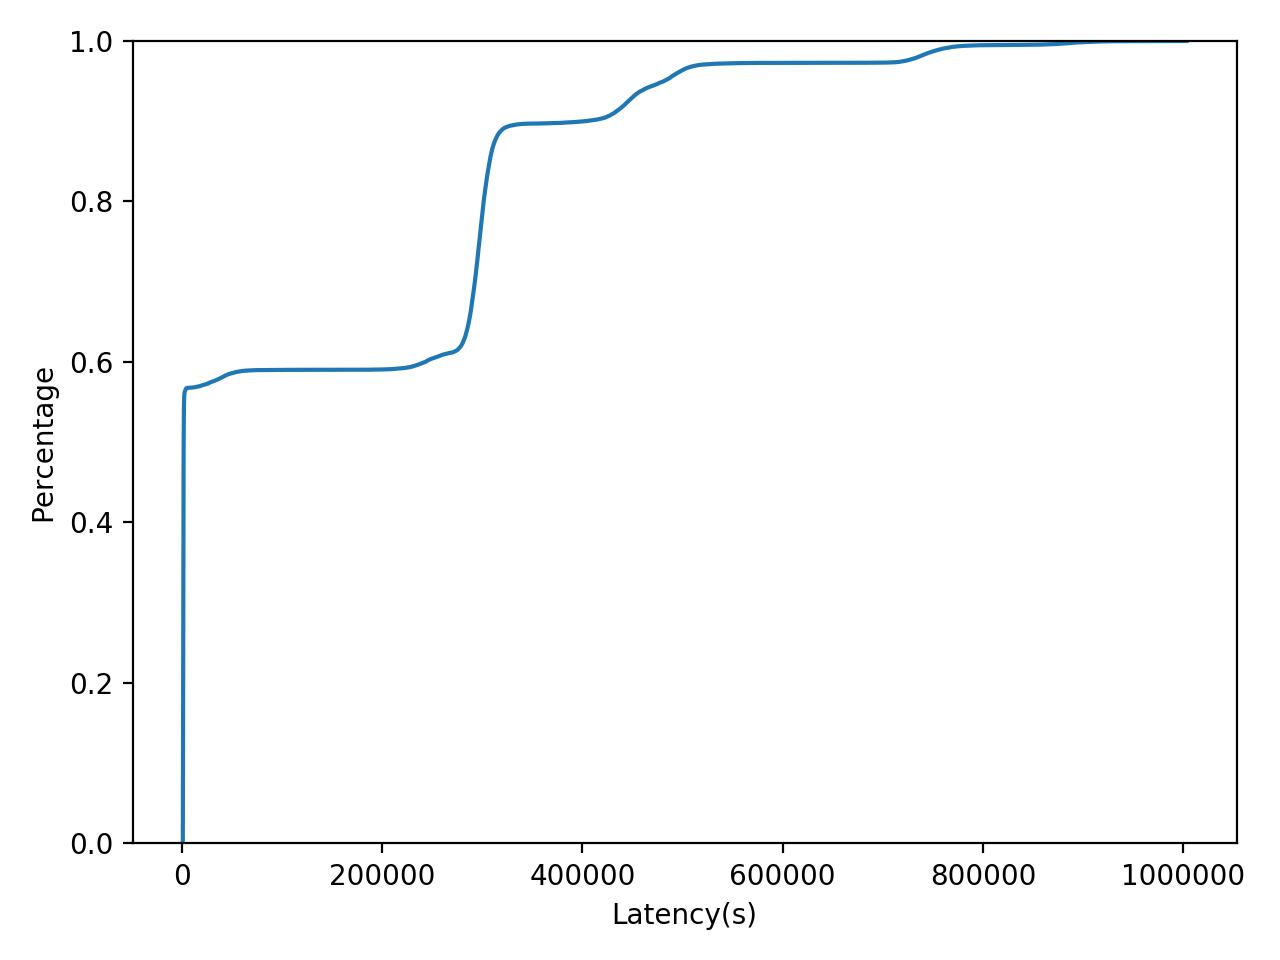
\includegraphics[width=0.49\textwidth,height=\textheight,keepaspectratio]{img/global50_lat.png}
%   \includegraphics[width=0.49\textwidth,height=\textheight,keepaspectratio]{img/global50_tp.png}
%   \includegraphics[width=0.49\textwidth,height=\textheight,keepaspectratio]{img/global10_lat.png}
%   \includegraphics[width=0.49\textwidth,height=\textheight,keepaspectratio]{img/global10_tp.png}
%   \includegraphics[width=0.49\textwidth,height=\textheight,keepaspectratio]{img/global5_lat.png}
%   \includegraphics[width=0.49\textwidth,height=\textheight,keepaspectratio]{img/global5_tp.png}
%   \includegraphics[width=0.49\textwidth,height=\textheight,keepaspectratio]{img/global1_lat.png}
%   \includegraphics[width=0.49\textwidth,height=\textheight,keepaspectratio]{img/global1_tp.png}
%   \caption{ global tests with 50, 90, 95 and 99 percent reads }
%   \label{fig:global50-performance}
% \end{figure}

% \begin{figure}[!htb]
%   \centering
%   \includegraphics[width=0.49\textwidth,height=\textheight,keepaspectratio]{img/global10_lat.png}
%   \includegraphics[width=0.49\textwidth,height=\textheight,keepaspectratio]{img/global10_tp.png}
%   \caption{ global test with 90\% reads }
%   \label{fig:global10-performance}
% \end{figure}

% \begin{figure}[!htb]
%   \centering
%   \includegraphics[width=0.49\textwidth,height=\textheight,keepaspectratio]{img/global5_lat.png}
%   \includegraphics[width=0.49\textwidth,height=\textheight,keepaspectratio]{img/global5_tp.png}
%   \caption{ global test with 95\% reads }
%   \label{fig:global5-performance}
% \end{figure}

% \begin{figure}[!htb]
%   \centering
%   \includegraphics[width=0.49\textwidth,height=\textheight,keepaspectratio]{img/global1_lat.png}
%   \includegraphics[width=0.49\textwidth,height=\textheight,keepaspectratio]{img/global1_tp.png}
%   \caption{ global test with 99\% reads }
%   \label{fig:global1-performance}
% \end{figure}
\newpage
The results of the global tests (Figure \ref{fig:global50-performance}) are as expected. The throughput are higher in the tests with more read operations. We don't see any improvements in throughput during the tests, because the nodes are by default assigned to all groups, and the loads of the clients are almost identical, which means that there is no real way to improve the partitioning. The latencies are on average worse than the tests with local skews, again as expected, since in those tests we were able to perform a partitioning that takes advantage of the locality.

Looking at the latencies there is an interesting stair-like shape, that gets less and less noticeable when increasing the reads. Those could be the plateaus given by the operations that require multiple groups to deliver the messages.

Table \ref{tab:global-latencies-table} shows the mean and various percentiles regarding the timing of operations for the global-skewed experiments. Again, they are in line with our observations made on the previous plots.
\vfill
\begin{table}[!htb]
  \centering
  \begin{tabular}{l l l l l l l l}
    \hline
    & \textbf{Mean} & \textbf{5\%} & \textbf{25\%} & \textbf{50\%} & \textbf{75\%} & \textbf{95\%}& \textbf{99\%} \\
    \hline
    \textbf{50\% reads} & 147.6 & 0.982 & 1.219 & 1.677 & 297.0 & 481.3 & 758.4 \\
    \textbf{90\% reads} & 151.4 & 1.045 & 1.990 & 43.58 & 243.3 & 527.7 & 768.5 \\
    \textbf{95\% reads} & 116.0 & 1.061 & 2.070 & 4.623 & 222.4 & 474.4 & 778.3 \\
    \textbf{99\% reads} & 68.02 & 1.340 & 2.316 & 3.087 & 4.990 & 366.3 & 698.4 \\
    \hline
  \end{tabular}
  \caption{Mean latency and percentiles regarding the global-skewed experiments}\label{tab:global-latencies-table}
\end{table}

\begin{figure}[H]
  \centering
  \includegraphics[width=0.49\textwidth,height=\textheight,keepaspectratio]{img/global50_lat.png}
  \includegraphics[width=0.49\textwidth,height=\textheight,keepaspectratio]{img/global50_tp.png}
  \includegraphics[width=0.49\textwidth,height=\textheight,keepaspectratio]{img/global10_lat.png}
  \includegraphics[width=0.49\textwidth,height=\textheight,keepaspectratio]{img/global10_tp.png}
  \includegraphics[width=0.49\textwidth,height=\textheight,keepaspectratio]{img/global5_lat.png}
  \includegraphics[width=0.49\textwidth,height=\textheight,keepaspectratio]{img/global5_tp.png}
  \includegraphics[width=0.49\textwidth,height=\textheight,keepaspectratio]{img/global1_lat.png}
  \includegraphics[width=0.49\textwidth,height=\textheight,keepaspectratio]{img/global1_tp.png}
  \caption{ CDF of latency on the left and throughput versus time on the right }
  \label{fig:global50-performance}
\end{figure}

\section{Constant}\label{sec:constant}
A third possible load would be a test with a flat distribution, achievable with a skew of $\alpha = 0$. This test would be a worst case scenario, since there are no different loads from the clients that can be exploited by the system to better distribute the objects. For this case we don't expect good performance, as probably most nodes will be assigned to the same partitions.

\begin{figure}[!htb]
  \centering
  \includegraphics[width=\textwidth,height=\textheight,keepaspectratio]{img/clients_loads_constant.png}
  \caption{ Distribution of client operations for the constant tests }
  \label{fig:constant-skewed-loads}
\end{figure}

% \begin{figure}[!htb]
%   \centering
%   \includegraphics[width=0.49\textwidth,height=\textheight,keepaspectratio]{img/constant10_lat.png}
%   \includegraphics[width=0.49\textwidth,height=\textheight,keepaspectratio]{img/constant10_tp.png}
%   \caption{ constant test with 90\% reads }
%   \label{fig:constant10-performance}
% \end{figure}

% \begin{figure}[!htb]
%   \centering
%   \includegraphics[width=0.49\textwidth,height=\textheight,keepaspectratio]{img/constant5_lat.png}
%   \includegraphics[width=0.49\textwidth,height=\textheight,keepaspectratio]{img/constant5_tp.png}
%   \caption{ constant test with 95\% reads }
%   \label{fig:constant5-performance}
% \end{figure}

% \begin{figure}[!htb]
%   \centering
%   \includegraphics[width=0.49\textwidth,height=\textheight,keepaspectratio]{img/constant1_lat.png}
%   \includegraphics[width=0.49\textwidth,height=\textheight,keepaspectratio]{img/constant1_tp.png}
%   \caption{ constant test with 99\% reads }
%   \label{fig:constant1-performance}
% \end{figure}

The results (Figure \ref{fig:constant50-performance}) are similar to the global-skewed, since in this case the clients have similar behavior as well. The observations made for the global tests apply to the constant tests as well. Interestingly, in the 50\% read test, the plateaus in the latencies are even more noticeable, perhaps because there's less variation in the combinations of group destinations.

Table \ref{tab:constant-latencies-table} shows the mean and percentiles for the constant experiments.

\begin{table}[!htb]
  \centering
  \begin{tabular}{l l l l l l l l}
    \hline
    & \textbf{Mean} & \textbf{5\%} & \textbf{25\%} & \textbf{50\%} & \textbf{75\%} & \textbf{95\%}& \textbf{99\%} \\
    \hline
    \textbf{50\% reads} & 99.26 & 0.874 & 1.140 & 1.820 & 222.8 & 342.2 & 948.1 \\
    \textbf{90\% reads} & 192.2 & 0.950 & 1.610 & 182.0 & 263.9 & 723.8 & 888.8 \\
    \textbf{95\% reads} & 132.5 & 1.006 & 1.543 & 3.196 & 238.5 & 479.0 & 833.4 \\
    \textbf{99\% reads} & 104.1 & 1.074 & 2.007 & 3.208 & 212.4 & 412.8 & 778.4 \\
    \hline
  \end{tabular}
  \caption{Mean latency and percentiles regarding the constant experiments}\label{tab:constant-latencies-table}
\end{table}


\begin{figure}[H]
  \centering
  \includegraphics[width=0.49\textwidth,height=\textheight,keepaspectratio]{img/constant50_lat.png}
  \includegraphics[width=0.49\textwidth,height=\textheight,keepaspectratio]{img/constant50_tp.png}
  \includegraphics[width=0.49\textwidth,height=\textheight,keepaspectratio]{img/constant10_lat.png}
  \includegraphics[width=0.49\textwidth,height=\textheight,keepaspectratio]{img/constant10_tp.png}
  \includegraphics[width=0.49\textwidth,height=\textheight,keepaspectratio]{img/constant5_lat.png}
  \includegraphics[width=0.49\textwidth,height=\textheight,keepaspectratio]{img/constant5_tp.png}
  \includegraphics[width=0.49\textwidth,height=\textheight,keepaspectratio]{img/constant1_lat.png}
  \includegraphics[width=0.49\textwidth,height=\textheight,keepaspectratio]{img/constant1_tp.png}
  \caption{ CDF of latency on the left and throughput versus time on the right }
  \label{fig:constant50-performance}
\end{figure}
\newpage
\section{Variable}\label{sec:variable}
This last test is slightly different, since this time we want to test if, and how quickly, the system adapts to a change in workloads. We will initially start with a local-skewed workload like in the first case, and after some time we will shift the clients once more, effectively changing the interest in the objects for all clients. What we expect to see is that after the workload changes the performance will drop, and after some repartitions the system will slowly move onto the new partitioning that increases the performance with the new workload. The change in workload is shown in Figure \ref{fig:variable-loads}.

The speed at which the system adapts to the new workload is highly dependant on the $\alpha$ variable used when updating the RW counters, which defines how quickly the RW counters age with every repartition. We use an $\alpha$ of $0.5$, as from our tests it looked like it was a fine compromise between adaptability and resiliance to unexpected behaviors. A slow adaptation to the new workload would be acceptable, since in our test we use the most abrupt change possible, which is quite unlikely in a normal execution.

Note that we performed this test only with the 50\% reads load, since what we want to see from this test is not related to the ratio of reads/writes, but just the behavior upon a change of client operations. The test is performed as follows: we start the system with the client loads as in the left image of Figure \ref{fig:variable-loads}. We perform a repartition after 1 minute, and then we repartition every 30 seconds. After 3 minutes and 30 seconds, when we expect the performance to be stable, we stop the clients, and start new ones with distributions as in the right image of Figure \ref{fig:variable-loads}. We then repeat the repartition after 1 minute and then 30 seconds, for at least a couple of minutes to see if the system recovers or not. 

\begin{figure}[!htb]
  \centering
  \includegraphics[width=0.49\textwidth,height=\textheight,keepaspectratio]{img/clients_loads.png}
  \includegraphics[width=0.49\textwidth,height=\textheight,keepaspectratio]{img/clients_loads_variable.png}
  \caption{ Distribution of client operations for the tests }
  \label{fig:variable-loads}
\end{figure}
The results, shown in Figure \ref{fig:variable50-performance}, are quite nice. The latency is nothing particularly different compared to the previous cases, as it shows a similar shape. The throughput instead is a positive result: in the right image of Figure \ref{fig:variable50-performance} we can see the purple line that represents the performance with the initial clients, and the pink line which represents the performance after we changed the client behavior. The purple line behaves as usual, with noticeable increments in performance at the 90 and 120 seconds mark, which correspond to two repartitions. Once we change the clients, the performance drops, since the partitioning is not optimal for the new clients. After the second repartition with the new clients, at 280 seconds, we see that the performance goes back up, meaning that the system adapted to the new clients, and that the repartition correctly re-assigned the nodes based on the recent operations of the new clients.

\begin{figure}[!htb]
  \centering
  \includegraphics[width=0.49\textwidth,height=\textheight,keepaspectratio]{img/variable50_lat.png}
  \includegraphics[width=0.49\textwidth,height=\textheight,keepaspectratio]{img/variable50_tp.png}
  \caption{ variable test with 50\% reads }
  \label{fig:variable50-performance}
\end{figure}

% \clearpage
\section{GeoPaxos results evaluation}\label{sec:geopaxos-results-evaluation}
Let us now analyze the results of the tests of the B+tree with GeoPaxos, and see if there are some interesting patterns or behaviors that are noteworthy.
\\\\
% \subsubsection{Read/write ratios performance}
As expected, in general the tests with more reads than writes show better performance. This is the expected behavior, since we don't always need to involve all the replicas that handle an object for a read operation, and furthermore GeoPaxos allows read operations to be performed in different orders in the case where the two operations do not conflict.
\\\\
% \subsubsection{Different partitionings}
One interesting exception happened in the local-skewed test, where the different ratio of reads and writes made it so that the nodes where partitioned differently, which ended up increasing the throughput by quite a noticeable margin. This is interesting because we were not expecting this to happen, but on further analyis it made sense that such a case could have happened.
\\\\
% \subsubsection{Resiliance}
Another interesting result is that the constant and global-skewed tests have their partitions and throughput almost costant troughout all the tests. What could have happened instead was that because of an uneven period of operations, one region could have monopolized the system, ending up with the repartitioning favoring this one region with an avalanche effect. Fortunately this did not happen, which means that the repartitioning is not too susceptible to such events.
\\\\
% \subsubsection{Plateaus}
Regarding the graphs of the latencies, we have plateaus which are particularly noticeable in the tests with few read operations. These can almost certainly be explained by the importance of multi-group operations. In the tests with 50\% writes, we have many occurrences where a message has to be ordered by a set of groups, which on average will have a latency cost that is highly dependant on the geographic location of the groups, and therefore the messages ordered by the same set of groups will have very similar latencies. Therefore, we will have that these operations are grouped together, ending up with the stair-like shape of the latency graphs. 
\\\\
% \subsubsection{Variable load}
The variable test case, which was the more peculiar one, showed good results as well. the system adapted quite quickly to the change in clients behavior, bringing the throughput back to normal levels after a couple of repartitions. This makes us think that the approach is definitely usable in more complicated and variable environments.
\\\\
% \subsubsection{Conclusion}
In conclusion, the tests showed positive behavior, with no particularly surprising results. Obviously the tests were hand-made and highly specific, therefore they can only give an approximate idea of the working of the system; further real world tests would have to be performed, with more complicated and realistic situations. Still, the results do show that the concept idea has some interesting qualities for possible future usages.

% Regarding the graphs of the latencies, we have plateaus which are particularly noticeable in the tests with few read operations. These can almost certainly explained by the importance of multi-group operations. In the tests with 50\% writes, we have many occurrences where a message has to be ordered by a set of groups, which on average will have a latency cost that is highly dependant on the geographic location of the groups, and therefore the messages ordered by the same set of groups will have very similar latencies. Therefore, we will have that these operations are grouped together, ending up with the stair-like shape of the latency graphs. 

% constant before a repartition is faster than local, because the loads are evenly distributed, less change to conflict keys
\chapter{Conclusion}\label{sec:Conclusion}
Let us now summarize what we have presented in this report and then draw some final conclusions.

We started by introducing the importance of distributed data structures in today's age, and in particular the benefits of using distributed trees such as B+trees. 

We then moved onto the core focus of this report, which is the efficient repartition of distributed B+tree data structures. We discussed what the challenges are, and how we planned to approach them.

Next we presented our different repartition algorithms, discussing the assumptions, limitations, and expectations we had of them. We proceeded by actually testing these repartition approaches. The tests were split into two big groups; the first group was aimed at testing only the repartition algorithms, so that we were able to assess the quality and efficiency of each method without the influence of other noise factors. The second group of tests was instead done with the distributed B+trees on top of GeoPaxos, to see how the repartition algorithms would have behaved in a more practical environment.

The results of the first tests were quite interesting, with some methods performing better than expected, and others falling short even though they looked good on paper. In general, though, all methods were able to bring some interesting improvements. The technique that was most impressive was the caching of the optimal partitions based on the given workloads of a node, in particular when paired with the hot groups optimization; this approach was able to improve the repartition times by up to a factor of 100 compared to the same algorithm without any caching mechanism. 

The tests with GeoPaxos were in line with our expectations, without any particularly big surprise. The chosen repartition algorithm (hot groups with LRU caching) did not appear to be a noticeable bottleneck at all, and the repartitions were able to improve the performance of GeoPaxos communications in the tests with advantageous clients behavior.

In conclusion, we definitely saw some viable methods to approach the repartition problem of distributed trees. The most interesting ones we found are the idea to cache repartition results and to discard the group combinations that are unlikely to matter. Putting these two approaches together we were able to only affect the repartition quality by negligible amounts, while drastically improve the efficiency of the repartition process.

\section{Future work}\label{sec:future-work}
Regarding what could be done in the future, there are various aspects that could be improved. 

One direction that could be interesting to follow is about implementing a more dynamic approach to the repartition algorithm. As we discussed in this report, we used one optimization approach at a time, and the results showed that most of them had pros and cons associated to them. Therefore a possible next step would be to make a system that has multiple methods available, and chooses which one to use depending on the state of the system. A simple example would be the case where the LRU cache is empty, in which case a fast method could be chosen, until the cache is filled up, and at that point it could be convenient to use the method that gives better quality of partitions.

Another possibility would be to attempt other completely different optimization approaches. In this report we presented a handful of ways to approximate and hence speed up the repartitions, usually based on some assumptions and heuristics. It is definitely possible to come up with alternative solutions, maybe based on different assumptions on the system.

Improving on the methods presented in this report is another possible track as well. This could be done in the way of actually changing and improving the concepts of the methods, or in further researching the optimal parameters that are necessary for the usage of some methods, such as optimizing the values of the treshold parameters.





% \chapter{Introduction}

% \lipsum



% \chapter[Short title]{A chapter title which will run over two lines --- it's for
%   testing purpose}

% \lipsum[1-2]

% \section{The first section}
% \lipsum[3-4]

%  \section{The second, math section}

% \textbf{Theorem 1 (Residue Theorem).}
% Let $f$ be analytic in the region $G$ except for the isolated singularities $a_1,a_2,\ldots,a_m$. If $\gamma$ is a closed rectifiable curve in $G$ which does not pass through any of the points $a_k$ and if $\gamma\approx 0$ in $G$ then
% \[
% \frac{1}{2\pi i}\int_\gamma f = \sum_{k=1}^m n(\gamma;a_k) \text{Res}(f;a_k).
% \]
% \textbf{Theorem 2 (Maximum Modulus).}
% \emph{Let $G$ be a bounded open set in $\mathbb{C}$ and suppose that $f$ is a continuous function on $G^-$ which is analytic in $G$. Then}
% \[
% \max\{|f(z)|:z\in G^-\}=\max \{|f(z)|:z\in \partial G \}.
% \]

% \section[third]{A very very long section, titled ``The third section'', with
%   a rather  short text alternative (third)}
% \lipsum \texttt{Some Test}
% \lstset{language=algebra,linewidth=0.95\linewidth,breaklines=true,numbers=left,
% basicstyle=\ttfamily,numberstyle=\tiny,escapeinside={//*}{\^^M},
% mathescape=true}
% \begin{lstlisting}
% import IntSpec, ItemSpec;

% sort cart; //*\label{sort}

% constructors //*\label{begin-sig}
% create() $\longrightarrow$ cart;
% insert(cart, item) $\longrightarrow$ cart;
% observers
% amount(cart) $\longrightarrow$ int;
% transformers
% delete(cart, item) $\longrightarrow$ cart; //*\label{end-sig}

% axioms //*\label{begin-axioms}
% forall c: cart, i, j: item 

% amount(create()) $=$ 0; //*\label{begin-amount}
% amount(insert(c,i)) $=$ amount(c) $+$ price(i); //*\label{end-amount}
% delete(create(),i) $=$ create(); //*\label{begin-delete}
% delete(insert(c,i),j) $=$
% if (i =$\:$= j) c
% else insert(delete(c,j),i); //*\label{end-axioms}
% end
% \end{lstlisting}

% As you can easily see from the above listing \citet{bbggs:iet07}
% define something weird based on the BPEL specification
% \citep{bpelspec}.
% \nocite{*}

% \appendix %optional, use only if you have an appendix

% \chapter{Some retarded material}
% \section{It's over\dots}
% \lipsum 

\backmatter

\chapter{Glossary} %optional

%\bibliographystyle{alpha}
%\bibliographystyle{dcu}
\bibliographystyle{plainnat}
\bibliography{biblio}

%\cleardoublepage
%\theindex %optional, use only if you have an index, must use
	  %\makeindex in the preamble
% \lipsum

\end{document}
